\documentclass[a4paper]{article}
\usepackage[
    lecture,
    course={Analysis~I},
    code={V1G1},
    lecturer={Prof.~Dr.\ Karl-Theodor Sturm},
    term={WS~2021/2022},
    noalgorithm, nolisting
]{tienuni}

\overfullrule3cm
\usetikzlibrary{math}
\usetikzlibrary{fit} %For `\tikzlastnode`

\begin{document}
\maketitle

\begin{footnotesize}
    Aktualisiert bis Vorlesung~18 am 15.~Dezember 2021.

    Ich weiß, dass das ein wenig spät kommt, aber ich hoffe, dass ihr einen Nutzen hieraus ziehen könnt. Ursprünglich wollte ich das nur für mich machen, aber da unser Dozent kein Skript hat, gebe ich meines heraus. Grundsätzlich ist der Inhalt der Vorlesung wiederzufinden, aber oft umformuliert und teilweise auch von mir etwas kommentiert. In den Fußnoten stehen meist Randinformationen, die über den Tellerrand hinausführen. Der Anhang sollte auch interessant werden.

    Orthografische und inhaltliche Errata sowie konstruktive Kommentare bitte an \url{mailto://Gargantuar314@uni-bonn.de}. Auch Vorschläge zur Formulierung, fehlende Kapitel und Ausführungen, Konsistenz oder sogar zur Typografie sind willkommen. Ich werde mal schauen, ob ich sie dann einarbeite. Über das Layout und die mathematische Formelsetzung werde ich aber kaum mit mir diskutieren lassen, insbesondere die reine Gestaltung in schwarz/weiß. Aber vielleicht wird mich noch einer umstimmen?

    Todo: Hinzufügen der fehlenden Beweise aus den Übungen. Vervollständigen des Anhangs. Vervollständigen der Schlagwortübersicht. Umsteigen auf \texttt{ntheorem}-Paket und Einrahmen von \texttt{theorem}-ähnlichen Umgebungen.
\end{footnotesize}

\begin{description}
    \item[Grundlagen] Aussagenlogik: logische Aussagen, Junktoren, Wahrheitstafeln, Tautologien. Beweisprinzip des indirekten Beweises. Prädikatenlogik: Quantoren, einige Regeln. Mengenlehre: Mengen, Element, Teilmenge, leere Menge, mengentheoretische Operatoren, Grenzen der naiven Mengenlehre.\hspace*{\fill}[1]
    \item[Vollständige Induktion] Beweisprinzip der vollständigen Induktion. Summen"~ und Produktzeichen. Fakultät, Binomialkoeffizient. Pascalsches Dreieck, binomischer Lehrsatz. Kombinatorik: Permutation, Kombination. Potenzmenge. Multinomialkoeffizient, Multinomialsatz.\hspace*{\fill}[1,5]
    \item[Körper der reellen Zahlen] Körperaxiome: Axiome eines Körpers, gefolgerte Rechenregeln, Verallgemeinerung der Assoziativität/Kommutativität/Distributivität. Anordnungsaxiome: Axiome der Anordnung, vergleichende Relationen, gefolgerte Rechenregeln. Archimedisches Axiom: Folgerungen, bernoullische Ungleichung. Betragsfunktion, Dreiecksungleichung.\hspace*{\fill}[1,5]
    \item[Konvergenz von Folgen~I] Begriffe: Folge, Konvergenz, Grenzwert/Limes, Beschränktheit. Grenzwertsätze. Ordnungserhaltung konvergenter Folgen.\hspace*{\fill}[1]
    \item[Vollständigkeitsaxiom] Cauchy-Folgen. Vollständigkeitsaxiom. Intervallschachtelung: Intervallschachtelungsprinzip, Existenz der Wurzeln. Supremumseigenschaft. Äquivalenz aller vier Ansätze. Ausblick zu~$\R$, Peano-Axiome von~$\N$. Abzählbarkeit.\hspace*{\fill}[2,5]
    \item[Konvergenz von Folgen~II] Monotone Folgen. Uneigentliche Konvergenz, erweiterte Zahlengerade. Limes Superior/Inferior. Teilfolgen, Häufungspunkte, Satz von Bolzano-Weierstraß.\hspace*{\fill}[1,5]
    \item[Konvergenz von Reihen] Reihen: harmonische/geometrische Reihe. Konvergenzkriterien: Cauchy-Kriterium, notwendige Bedingung einer Nullfolge, monoton und beschränkt, Leibniz-Kriterium, Majorantenkriterium, Quotientenkriterium, Wurzelkriterium. Riemmansche Zeta-Funktion.\hspace*{\fill}[1]
    \item[Absolut konvergente Reihen, summierbare Familien] Absolut konvergente Reihen. Umordnung: Umordnungssatz. Summierbare Familien: großer Umordnungssatz, Doppelreihensatz. Produkt von Reihen: Faltung, Cauchy-Produkt. Binomische Reihe.\hspace*{\fill}[2]
    \item[Exponentialreihe] Exponentialreihe: absolut konvergent, eulersche Zahl. Restgliedabschätzung. Funktionalgleichung. Abschätzungen von~$\exp$. Grenzwertdarstellung.\hspace*{\fill}[1]
    \item[Komplexe Zahlen] Körper der komplexen Zahlen: Rechenregeln, komplexe Zahlenebene, Ähnlichkeit zu~$\R^2$. Komplexe Konjugation, Betrag: Rechenregeln, Ungleichungen. Folgen in~$\C$: Cauchy-Folgen, Grenzwertsätze, auch bzgl.\ Konjugation und Betrag. Reihen in~$\C$: Konvergenzkriterien. Exponentialreihe. Trigonometrische und hyperbolische Funktionen: Reihendarstellung, Identitäten (eulersche Formel, trigonometrischer Pythagoras), Additionstheoreme, Doppelwinkelfunktionen. Trigonometrische und hyperbolische Funktionen in~$\R$, Abschätzungen. Kreiszahl~$\pi$: Verhältnis zu $\exp$/$\sin$/$\cos$, Periodizität, Phasenverschiebung, Nullstellen von $\sin$/$\cos$ in~$\C$. Polardarstellung: Multiplikation. Einheitswurzeln.\hspace*{\fill}[3]
    \item[Stetige Funktionen] Funktionsbegriff: Beispiele, algebraische Operationen, Komposition, Umkehrung. Stetigkeit: $\eps$"~$\delta$"~Kriterium, Folgenkriterium, Äquivalenz beider. Folgerungen: Stetigkeit bekannter Funktionen ($\exp$, Wurzel, Konstante, Identität, Betrag, Polynom, rationale Funktion), Stetigkeit unter algebraischen Operationen/Komposition. 
\end{description}

\newpage\tableofcontents

\section{Grundlagen}

Wir werden uns zuerst mit einigen notwendigen logischen und mengentheoretischen Grundlagen beschäftigen. Dabei steigen wir nicht zu tief in die Materie ein, sondern behandeln alles (für unsere Zwecke ausreichend) etwas oberflächlich. Einen rigoroseren Zugang findet man in der Literatur dieser Gebiete.

\subsection{Aussagenlogik}

\begin{definition}[Aussage]
    Eine \emph{Aussage} ist ein mathematischer oder sprachlicher Satz, der entweder \emph{wahr}~(1) oder \emph{falsch}~(0) ist.
\end{definition}

Aussagen drücken damit keine Wahrscheinlichkeiten und auch kein "`vielleicht"' aus. Ziel der Aussagenlogik ist es, aus gegebenen Aussagen neue (wahre) Aussagen abzuleiten.

\begin{definition}[logische Operatoren, Junktoren]
    Seien $A$~und~$B$ zwei Aussagen. Es werden folgende Operatoren
    \begin{center}
        \begin{tabular}{@{}lll@{}}\toprule
            Symbol                & Name               & Gesprochen                                                             \\\midrule
            $\neg A$              & \emph{Negation}    & "`nicht~$A$"'                                                          \\
            $A \wedge B$          & \emph{Konjunktion} & "`$A$~und~$B$"', "`sowohl~$A$ als auch~$B$"'                           \\
            $A \vee B$            & \emph{Disjunktion} & "`$A$~oder~$B$"' (dabei ist \emph{nicht} das Exklusive Oder gemeint)   \\
            $A \Rightarrow B$     & \emph{Implikation} & "`aus~$A$ folgt~$B$"', "`$A$~impliziert~$B$"', "`wenn~$A$, dann~$B$"'  \\
            $A \Leftrightarrow B$ & \emph{Äquivalenz}  & "`$A$~ist äquivalent zu~$B$"', "`$A$~genau dann, wenn~$B$"',           \\
                                  &                    & "`$A$~dann und nur dann, wenn~$B$"' (engl.\ "`iff~-- if and only if"') \\\bottomrule
        \end{tabular}
    \end{center}
    durch die folgende \emph{Wahrheitstafel} definiert:
    \begin{center}
        \begin{tabular}{@{}cc@{\colsep}ccccc@{}}\toprule
            $A$ & $B$ & $\neg A$ & $A \wedge B$ & $A \vee B$ & $A \Rightarrow B$ & $A \Leftrightarrow B$ \\\midrule
            w   & w   & f        & w            & w          & w                 & w                     \\
            w   & f   & f        & f            & w          & f                 & f                     \\
            f   & w   & w        & f            & w          & w                 & f                     \\
            f   & f   & w        & f            & f          & w                 & w                     \\\bottomrule
        \end{tabular}
    \end{center}
\end{definition}

Wir können uns die Wahrheitswerte wie folgt merken:
\begin{itemize}
    \item $\neg A$ dreht den Wahrheitswert um.

          Das macht Sinn, denn wenn eine Aussage wahr war, wird sie danach falsch und andersherum.
    \item $A \vee B$ ist nur wahr, sobald eine der beiden oder beide Aussagen wahr ist. \emph{Achtung}: Hiermit ist nicht das Exklusive Oder (auch "`entweder~\dots oder"') gemeint, dass falsch ist, wenn beide Aussagen wahr sind.

          Auch das macht Sinn, denn wenn ich z.\,B.\ das eine \emph{oder} das andere möchte, dann ist es egal, was von beiden eintritt~-- ich bin mit beiden zufrieden. Unzufrieden wäre ich hingegen, wenn weder das eine noch das andere eintritt.
    \item $A \wedge B$ ist nur wahr, wenn beide Aussagen wahr sind.

          Auch das macht Sinn: Wenn die Zitrone gelb und der Himmel blau ist, dann müssen schon beide Aussagen stimmen, damit diese Aussage insgesamt als richtig angesehen werden kann.
    \item $A \Rightarrow B$ ist nur falsch, wenn aus einem wahren~$A$ ein falsches~$B$ gefolgert wird. D.\,h., dass aus einer falschen Aussage alles gefolgert werden kann,\footnote{Lat.\ \emph{ex falso quodlibet}~-- "`aus Falschem folgt Beliebiges"'.} wohingegen aus einer wahren Aussage nur wahre Aussagen folgen.

          Das macht auch Sinn, denn wenn es regnet, ist die Straße zwar nass, aber wenn es nicht regnet, kann die Straße trotzdem nass sein (wenn z.\,B.\ jemand Wasser auf die Straße schüttete).
    \item $A \Leftrightarrow B$ ist genau dann wahr, wenn $A$ und~$B$ denselben Wahrheitswert besitzen.

          Das macht Sinn, denn wenn zwei Dinge äquivalent ("`gleich"') sind, dann sollte man sie sich gegenseitig ersetzen können.
\end{itemize}

\subsubsection{Gesetze der Aussagenlogik}

\begin{definition}[Tautologie]
    Eine \emph{Tautologie} ist eine Aussage, die immer wahr ist~-- unabhängig vom Wahrheitswert der darin enthaltenen Aussagen.
\end{definition}

Tautologien, die eine Äquivalenz von Aussagen darstellen, können verwendet werden, um logische Aussagen äquivalent umzuformen und damit syntaktisch zu vereinfachen.

\begin{theorem}[Kontraposition]\label{thm:contraposition}
    Für zwei Aussagen $A$~und~$B$ gilt
    \begin{equation*}
        (A \Rightarrow B) \iff (\neg B \Rightarrow \neg A).
    \end{equation*}
\end{theorem}

\begin{theorem}\label{thm:implication}
    Für zwei Aussagen $A$~und~$B$ gilt
    \begin{equation*}
        (A \Rightarrow B) \iff (\neg A \vee B).
    \end{equation*}
\end{theorem}

\begin{proof}[Beweis zu \cref{thm:implication}]
    Wir beweisen den Satz mithilfe einer Wahrheitstafel.
    \begin{center}
        \begin{tabular}{@{}cc@{\colsep}cc@{}}\toprule
            $A$ & $B$ & $A \Rightarrow B$ & $\neg A \vee B$ \\\midrule
            w   & w   & w                 & w               \\
            w   & f   & f                 & f               \\
            f   & w   & w                 & w               \\
            f   & f   & w                 & w               \\\bottomrule
        \end{tabular}
    \end{center}
    Die Äquivalenz der beiden letzten Spalten ist stets wahr.
\end{proof}

Treten in einer zu zeigenden Tautologie noch mehr Aussagen auf, wächst die Wahrheitstafel dementsprechend um mehr Zeilen. Bei z.\,B.\ drei Aussagen $A$,~$B$ und~$C$ sind es schon $2^3 = 8$~Zeilen.

\begin{theorem}\label{thm:logiclaws}
    Weitere Tautologien und Schlussregeln, die oft verwendet werden:\footnote{
        Noch weitere (nicht triviale) hilfreiche Tautologien, die der Dozent leider nicht nannte, sind
        \begin{align*}
                                &                                     & A \Rightarrow (B \Leftrightarrow C) & \iff (A \Rightarrow B) \Rightarrow (A \Rightarrow C)                                             \\
                                &                                     & \iff A \Rightarrow (Q \wedge R)     & (A \Rightarrow B) \wedge (A \Rightarrow C)                                                       \\
                                &                                     & A                                   & \iff \neg (\neg A)                                   &  & \text{doppelte Negation},              \\
            A \wedge (B \vee C) & \iff (A \wedge B) \vee (A \wedge C) & A \vee (B \wedge C)                 & \iff (A \vee B) \wedge (A \vee C)                    &  & \text{Distributivität},                \\
            A \wedge (A \vee B) & \iff A                              & A \vee (A \wedge B)                 & \iff A                                               &  & \text{Absorption},                     \\
            \neg (A \wedge B)   & \iff (\neg A \vee \neg B)           & \neg (A \vee B)                     & \iff (\neg A \wedge \neg B)                          &  & \text{\textsc{de-morgansche} Gesetze}. \\
        \end{align*}
    } Seien $A$,~$B$ und~$C$ Aussagen. Dann gelten
    \begin{align*}
         & (A \Leftrightarrow B) \iff (\neg A \Leftrightarrow \neg B),                                                                                    \\
         & ((A \Rightarrow B) \wedge A) \implies B                                 &  & \text{\emph{Modus ponens} (Prinzip der vollständigen Induktion),} \\
         & ((A \Rightarrow B) \wedge \neg B) \implies \neg A                       &  & \text{\emph{Modus tollens} (Prinzip des indirekten Beweises),}    \\
         & ((A \Rightarrow B) \wedge (B \Rightarrow C)) \implies (A \Rightarrow C) &  & \text{\emph{Hypothetischer Syllogismus},}                         \\
         & A \implies (A \vee B),                                                                                                                         \\
         & \neg A \implies (A \Rightarrow B).
    \end{align*}
\end{theorem}

\subsubsection{Indirekter Beweis}

Aufbauend auf \cref{thm:contraposition} bzw.\ dem \emph{Modus tollens} aus \cref{thm:logiclaws} lässt sich das Beweisprinzip des \emph{indirekten Beweises} (auch \emph{Widerspruchsbeweis}, \emph{reduction ad absurdum}) formulieren.

Wir wollen die Aussage~$A \implies B$ beweisen. Dafür
\begin{itemize}
    \item nehmen wir an, dass die Annahme~$\neg B$ gilt und
    \item führen das zum Widerspruch mit~$A$ (wir erhalten $\neg B \implies \neg A$, was im Widerspruch zum wahren~$A$ steht).
\end{itemize}

\begin{example}
    \emph{Satz von \textsc{Euklid}: Es gibt unendlich viele Primzahlen.}

    \emph{Beweis}: Angenommen es gibt nur endlich viele Primzahlen $p_1, p_2, \dots, p_n$. Die Zahl $m = p_1 p_2 \dots p_n + 1$ ist aber durch keine der obigen Primzahlen teilbar, weshalb $m$ selbst eine Primzahl ist. Folglich gibt es mehr Primzahlen als die $p_1, p_2, \dots, p_n$, ein Widerspruch, weshalb die Annahme falsch ist und somit unendlich viele Primzahlen existieren.
\end{example}

\subsection{Prädikatenlogik}

\begin{definition}[Aussageform]
    Aussagen, die von freien Variablen abhängen, heißen \emph{Aussageformen}.
\end{definition}

Eine Aussageform besitzt keinen Wahrheitswert. Nach Einsetzen in die Variablen wird die Aussageform zur Aussage und wir können dann einen Wahrheitswert zuordnen.

\begin{example}\label{ex:propformula}\leavevmode
    \begin{enumerate}
        \item Es gibt (mindestens) eine reelle Zahl~$x$ mit $x^2 + 1 = 0$.\label{ex:exists}
        \item Für alle natürlichen Zahlen~$x$ gilt $x^2 - 1 = (x - 1) (x + 1)$.\label{ex:forall}
    \end{enumerate}
    Die Gleichungen $x^2 + 1 = 0$ und $x^2 - 1 = (x - 1) (x + 1)$ sind Aussageformen. Erst nach Einsetzen gewisser~$x$ können wir bestimmen, ob sie wahr sind. Es stellt sich heraus, dass es kein~$x$ gibt, für das die erste Gleichung wahr ist, und alle~$x$ die zweite Gleichung erfüllen. Deshalb ist \cref{ex:exists} falsch und \cref{ex:forall} wahr.
\end{example}

\begin{notation}[Quantoren]
    Wir schreiben kürzer
    \begin{itemize}
        \item $\exists$~(\emph{Existenzquantor}) für "`es gibt ein"' oder "`es existiert ein"' und
        \item $\forall$~(\emph{Allquantor}) für "`für alle"'.
    \end{itemize}
\end{notation}

Damit können wir die Aussagen aus dem obigen \cref{ex:propformula} mit den Quantoren durch
\begin{itemize}
    \item $\exists x \in \R\colon x^2 + 1 = 0$ und
    \item $\forall x \in \N\colon x^2 - 1 = (x - 1) (x + 1)$
\end{itemize}
ausdrücken.

\begin{theorem}[einige Regeln über Quantoren]\leavevmode
    \begin{enumerate}
        \item Quantoren lassen sich negieren. Sei hierfür $A(x)$ eine Aussage in~$x$. Dann gilt
              \begin{equation*}
                  \neg (\forall x\colon A(x)) \iff (\exists x\colon \neg A(x)), \quad\text{daher auch}\quad \neg (\exists x\colon A(x)) \iff (\forall x\colon \neg A(x)).
              \end{equation*}
              Auch gilt für eine Aussage~$A(x, y)$ in $x$~und~$y$
              \begin{equation*}
                  \neg (\exists x\colon \forall y\colon A(x, y)) \iff (\forall x\colon \exists y\colon \neg A(x, y)) \quad\text{und}\quad \neg (\forall x\colon \exists y\colon A(x, y)) \iff (\exists x\colon \forall y\colon \neg A(x, y)).
              \end{equation*}
        \item Quantoren lassen sich vertauschen. Sei $A(x, y)$ eine Aussage in $x$~und~$y$. Es gilt
              \begin{equation*}
                  (\exists x\colon \forall y\colon A(x, y)) \implies (\forall y\colon \exists x\colon A(x, y)).
              \end{equation*}
        \item Für zwei Aussagen $A(x)$ und~$B(x)$ in~$x$ gilt
              \begin{equation*}
                  (\exists x\colon A(x) \wedge B(x)) \implies ((\exists x\colon A(x)) \wedge (\exists x\colon B(x))).
              \end{equation*}
        \item Im Allgemeinen gilt für eine Aussage~$A(x)$ über eine Menge~$M$ \underline{\emph{nicht}}
              \begin{equation*}
                  (\forall x \in M\colon A(x)) \implies (\exists x \in M\colon A(x)).
              \end{equation*}
    \end{enumerate}
\end{theorem}

\begin{remark}
    Theoretisch lassen sich diese Aussagen korrekt beweisen, worauf wir hier aber verzichten werden. Trotzdem einige Bemerkungen:
    \begin{enumerate}
        \item Um eine Aussage mit beliebig vielen Quantoren zu verneinen, müssen wir uns von vorne nach hinten durcharbeiten und jeden All"- durch einen Existenzquantor ersetzen und andersherum. Zu allerletzt wird $A(x)$ bzw.~$A(x, y)$ negiert.

              Das bedeutet auch insbesondere, dass wenn eine Allaussage falsch sein soll, nur ein \emph{Gegenbeispiel} reicht. Ist hingegen ein Existenzaussage falsch, so müssen wir zeigen, dass \emph{alle} Objekte die gegebene Eigenschaft nicht erfüllen.
        \item Ein Existenz"~ vor einem Allquantor lässt sich vertauschen. Wenn es ein~$x$ gibt, sodass $A(x, y)$ für alle~$y$ gilt, so gibt es für jedes~$y$ auch ein~$x$~-- nämlich erfüllt stets dasselbe~$x$ die Aussage~$A(x, y)$. Die Umkehrung gilt hingegen im Allgemeinen \emph{nicht}, da wenn es für jedes~$y$ zwar ein~$x$ gibt, es noch lange nicht für jedes~$y$ stets dasselbe~$x$ sein muss. \emph{Beispiel}: Für~$x = 0$ und allen~$y \in \N$ gilt~$A(x ,y)$. Dann gibt es für jedes~$y \in \N$ auch ein~$x$, nämlich stets dasselbe~$x = 0$. Gibt es hingegen für jedes~$y \in \N$ ein~$x$, so gilt die Umkehrung nicht, da für~$y = 1$ z.\,B.~$x = 1$, für~$y = 2$ aber z.\,B.~$x = 2$ die Aussage~$A(x, y)$ erfüllt und wir somit nicht mit Sicherheit sagen können, dass ein~$x$ existiert, für das~$A(x, y)$ für alle~$y$ wahr ist.
        \item Der Existenzquantor kann distributiv auf eine Konjunktion verteilt werden. Wenn ein~$x$ sowohl~$A(x)$ als auch~$B(x)$ erfüllt, so erfüllt selbstverständlich dasselbe~$x$ auch $A(x)$ und~$B(x)$ getrennt voneinander. Die Umkehrung gilt hingegen \emph{nicht}: Denn ein~$x$, dass $A(x)$ erfüllt, und ein~$x$, dass $B(x)$ erfüllt, muss nicht dasselbe sein.
        \item Ein Allquantor impliziert im Allgemeinen nicht den Existenzquantor. \emph{Gegenbeispiel}: Die Menge~$M$ könnte ja leer sein.
    \end{enumerate}
\end{remark}

\subsection{Mengenlehre}

Für unsere Zwecke reicht die naive Mengenlehre, begründet durch \textsc{Georg Cantor}.

\begin{definition}[naive Menge und Elemente]
    Eine \emph{Menge} ist die Zusammenfassung bestimmter wohlunterscheidbarer Objekte unserer Anschauung oder unseres Denkens (welche die \emph{Elemente} der Menge genannt werden) zu einem Ganzen.
\end{definition}

\begin{example}\leavevmode
    \begin{itemize}
        \item Menge der natürlichen Zahlen $\N = \mset{1, 2, 3, \dots}$ (für diese Vorlesung beginnend bei~1), $\N_0 = \mset{0, 1, 2, 3, \dots}$
        \item $M = \mset{x \in \R : A(x)}$ für die Menge aller reellen Zahlen, für die $A(x)$ gilt
        \item $M = \mset{a, b, c, d}$ als einfache Auflistung
    \end{itemize}
\end{example}

\begin{notation}
    Für zwei Mengen $M$~und~$N$ bezeichnen
    \begin{itemize}
        \item $x \in M$ "`\emph{ist Element von}"',
        \item $M \subset N$ die \emph{Teilmenge}~$M$, jedes Element von~$M$ ist auch in~$N$ enthalten (nicht notwendigerweise echt, d.\,h.\ nicht notwendigerweise~$M \neq N$),
        \item $M \subsetneq N$ die \emph{echte Teilmenge}~$M$, also $M \subset N$ und~$M \neq N$, und
        \item $\varnothing = \mset{}$ die \emph{leere Menge}, die keine Elemente enthält ($\varnothing$~ist \emph{nicht}~$\mset{0}$).
    \end{itemize}
\end{notation}

\begin{definition}[mengentheoretische Operatoren]
    Für zwei Mengen $M$~und~$N$ werden folgende mengentheoretische Operatoren definiert:
    \begin{center}
        \begin{tabular}{@{}lll@{}}\toprule
            Symbol                       & Name                & Definition                                                               \\\midrule
            $M \cap N$                   & \emph{Durchschnitt} & $\mset{x : (x \in M) \text{ und } (x \in N)}$                            \\
            $M \cup N$                   & \emph{Vereinigung}  & $\mset{x : (x \in M) \text{ oder } (x \in N)}$                           \\
            $N^C = \complement N$        & \emph{Komplement}   & $\mset{x \in X : x \notin N}$ für eine übergeordnete Menge $X \supset N$ \\
            $M \setminus N = M \cap N^C$ & \emph{Differenz}    & $\mset{x \in M : x \notin N}$                                            \\\bottomrule
        \end{tabular}
    \end{center}
\end{definition}

\begin{figure}
    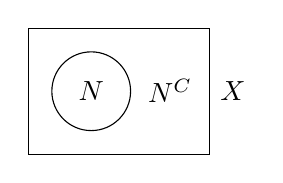
\begin{tikzpicture}
        \draw (0,0) circle [radius=0.5];
        \node at (0,0) {$N$};
        \draw (-0.8,-0.8) rectangle (1.5,0.8);
        \node at (1,0) {$N^C$};
        \node at (1.8,0) {$X$};
    \end{tikzpicture}
    \caption{Komplementmenge~$N^C = \complement N$.}
\end{figure}

\begin{definition}[disjunkt]
    Zwei Mengen $M$~und~$N$ heißen \emph{disjunkt}, falls $M \cap N = \varnothing$ gilt.
\end{definition}

Die optische Ähnlichkeit der mengentheoretischen Operatoren $\wedge$~und~$\vee$ mit den logischen Operatoren $\cap$~und~$\cup$ ist kein Zufall. Bspw.\ gilt
\begin{gather*}
    \mset{x \in M : A(x) \wedge B(x)} = \mset{x \in M : A(x)} \cap \mset{x \in M : B(x)}, \\
    \mset{x \in M : A(x) \vee B(x)} = \mset{x \in M : A(x)} \cup \mset{x \in M : B(x)}.
\end{gather*}

\subsubsection{Grenzen der naiven Mengenlehre}

Im Laufe der Mathematikgeschichte stellte sich leider heraus, dass die naive Mengenlehre\footnote{Eigentlich mehrere naive Mengenlehren, wie z.\,B.\ von \textsc{Georg Cantor}, \textsc{Richard Dedekind} oder \textsc{Gottlob Frege}.} sich zu unklar über erlaubte und nicht erlaubte Mengenbildungen äußert. Die Mengendefinition lässt also einen Interpretationsspielraum, was zu Widersprüchen führen kann.\footnote{Später wurde sie durch axiomatische Systeme ersetzt (\emph{\textsc{Zermelo}-\textsc{Faenkel}-Mengenlehre}).}

Nicht erlaubt ist z.\,B.\ die Konstruktion der Mengen~$M$ aller Mengen, die sich nicht selbst als Element enthalten (\emph{\textsc{russellsche} Antinomie}). Es stellt sich die Frage, ob $M$ sich selbst enthält oder nicht: Alle Elemente von~$M$ haben per Definition die Eigenschaft, dass sie sich selbst nicht enthalten. Gilt~$M \in M$, so kann~$M$ sich nach Definition nicht selbst enthalten, Widerspruch! Gilt~$M \notin M$, so muss~$M$ nach Definition sich selbst enthalten, Widerspruch! Eine solche Konstruktion ist also unmöglich.

Analog dazu formulierte \textsc{Bertrand Russel} das \emph{Barbierproblem}: Der Barbier ist derjenige, der ausschließlich all diejenigen rasiert, die sich nicht selbst rasieren. Rasiert er sich? Das führt unumgänglich zu einem Paradox.\footnote{Eine interessante Anekdote aus \textsc{Paul~R.\ Halmos'} \emph{Naive Mengenlehre} dazu befindet sich in \cref{apx:russell}.}

\iffalse
\subsection{Übungsaufgaben}

\begin{problem}[B01.A1]\leavevmode
\begin{enumerate}
    \item Es sei $A$~die Aussage "`Falls die Sonne scheint, gehen wir baden"'. Welche der Aussagen $A_1$~bis~$A_3$ folgen aus~$A$?
          \begin{enumerate}
              \item[$A_1$] "`Falls wir baden gehen, scheint die Sonne."'
              \item[$A_2$] "`Falls die Sonne nicht schient, gehen wir nicht baden."'
              \item[$A_3$] "`Falls wir nicht baden gehen, scheint nicht die Sonne."'
          \end{enumerate}
    \item Es sei~$B$ die Aussage: "`Es gibt eine Partei, in der jeder Politiker alle Gesetze des Steuerrechts kennt"'. Formulieren Sie diese Aussage mit Quantoren. Geben Sie sowohl in Quantorenschreibweise als auch in Umgangssprache die Negation~$\neg B$ an.
\end{enumerate}
\end{problem}

\begin{solution}\leavevmode
    \begin{enumerate}
        \begin{enumerate}
            \item[$A_1$] \emph{Aus~$A$ folgt nicht~$A_1$.} $A$~macht nur eine Aussage über den Fall, dass die Sonne scheint. Wir können auch aus einem anderen Grund baden gehen, z.\,B.\ wenn ein Freund Geburtstag hat. Dann muss aber nicht notwendigerweise die Sonne scheinen. \emph{Die Konversion (Umkehrung) gilt nicht immer.}
            \item[$A_2$] \emph{Aus~$A$ folgt nicht~$A_2$.} $A$~macht nur eine Aussage über den Fall, dass die Sonne scheint. Scheint die Sonne nicht, könnte alles passieren~-- wir könnten trotzdem baden gehen. \emph{Eine Implikation ist eine Äquivalenz.}
            \item[$A_3$] \emph{Aus~$A$ folgt~$A_3$.} Würde nämlich die Sonne scheinen, so gehen wir nach~$A$ baden, was aber der Voraussetzung widerspricht. \emph{Implikation und Kontraposition sind (tautologisch) äquivalent.}
        \end{enumerate}
        \item Die Aussage~$B$ und dessen Negation~$\neg B$ sind
              \begin{gather*}
                  \exists\text{Partei}\in(\text{Menge aller Parteien})\colon \forall\text{Politiker}\in\text{Partei}\colon \forall\text{Gesetz}\in\text{Steuerrecht}\colon (\text{Politiker kennt Gesetz}), \\
                  \forall\text{Partei}\in(\text{Menge aller Parteien})\colon \exists\text{Politiker}\in\text{Partei}\colon \exists\text{Gesetz}\in\text{Steuerrecht}\colon \neg(\text{Politiker kennt Gesetz}).
              \end{gather*}
              $\neg B$~umgangssprachlich formuliert: "`In jeder Partei gibt es einen Politiker, der ein Gesetz des Steuerrechts nicht kennt".'
    \end{enumerate}
\end{solution}

\begin{problem}[B01.A2]
Seien $A$,~$B$ und~$C$ beliebige Aussagen. Beweisen Sie durch geeignete Umformungen, d.\,h.\ unter Verwendung der Gesetze der Aussagenlogik, und mit Hilfe einer Wahrheitstabelle, dass
\begin{enumerate}
    \item $[(A \vee \neg B) \Leftrightarrow (\neg(A \wedge B) \vee (\neg B \wedge C))] = \neg B$,
    \item $[A \Rightarrow (B \Leftrightarrow C)] = [(A \Rightarrow B) \Leftrightarrow (A \Rightarrow C)]$.
\end{enumerate}
\end{problem}

\begin{problem}[B01.A3]
Seien $A$~und~$B$ beliebige Aussagen. Beweisen Sie durch geeignete Umformungen, d.\,h.\ unter Verwendung der Gesetze der Aussagenlogik, und mit Hilfe einer Wahrheitstabelle, dass
\begin{enumerate}
    \item $[A \Leftrightarrow B] = [(\neg A \wedge \neg B) \vee (A \wedge B)]$,
    \item $(A \Rightarrow B) \Leftrightarrow (\neg B \Rightarrow \neg A)$ eine Tautologie ist, d.\,h.\ die Wahrheitsfunktion dieser Aussage ist identisch "`WAHR"'.
\end{enumerate}
\end{problem}

\begin{problem}[B01.P1]\leavevmode
\begin{enumerate}
    \item Multiplizieren Sie aus:
          \begin{enumerate}
              \item $(y-3) (y+6)$,
              \item $(a-b) (a^2 + ab + b^2)$,
              \item $(a+2)^2$,
              \item $(a-b)^3$,
              \item $(a-b)^2 (a+b)$.
          \end{enumerate}
    \item Fassen Sie zu einem Produkt zusammen:
          \begin{enumerate}
              \item $ac + 2c - ad - 2d$,
              \item $a^2 + 3ab + 2b^2$,
              \item $12ax + 6ay + 20bx + 10by$,
              \item $a^3 - b^3$,
              \item $1 + a + a^2 + a^3$.
          \end{enumerate}
    \item Vereinfachen Sie unter geeigneten Einschränkungen an den Definitionsbereich der Variablen.
          \begin{enumerate}
              \item $\displaystyle 1-\frac{n-1}{n}$,
              \item $\displaystyle \frac{1}{1 + 1/x}$,
              \item $\displaystyle \frac{1}{a+b} \paren*{\frac{1}{ab^2} + \frac{1}{a^2b}}$,
              \item $\displaystyle \paren*{\frac{4}{xy} + \frac{3}{yz}} \paren*{\frac{xz-y}{y} + 1}$,
              \item $\displaystyle \frac{x/y - z/x}{2/x - z/y}$.
          \end{enumerate}
\end{enumerate}
\end{problem}

\begin{problem}[B01.P2]
Für~$x \in \R$ ist der \emph{Absolutbetrag} (oder auch \emph{Betrag}) von~$x$ definiert durch
\begin{equation*}
    \abs{x} =
    \begin{cases}
        x  & \text{falls } x \geq 0, \\
        -x & \text{sonst}.
    \end{cases}
\end{equation*}

Bestimmen Sie die Lösungsmenge der folgenden Gleichungen.
\begin{enumerate}
    \item $x^2 + x - 6 = 0$,
    \item $\abs{x+1} = x+2$,
    \item $x^2 - 4x + 5 = 3x^2 + 7$,
    \item $-3\abs{x-2} = 3x+1$,
    \item $x^2 = x+1$.
\end{enumerate}
\end{problem}
\fi

\section{Vollständige Induktion}

Die \emph{vollständige Induktion} ist ein mächtiges Beweisverfahren, was sehr oft Anwendung findet. Ist $A(n)$~eine Aussage, die für alle~$n \in \N$ gelten soll, können wir nicht nacheinander unendlich viele $A(1), A(2), \dots$ zeigen. Das Beweisverfahren schafft es aber, die Aussage \emph{für alle~$n$} zu zeigen.

\subsection{Beweisprinzip der vollständigen Induktion}\label{subsec:induction}

Wir setzen die Menge der natürlichen Zahlen $\N = \mset{1, 2, 3, \dots}$ vor. Die Aussage~$A(n)$ gilt für alle~$n \in \N$, falls:
\begin{enumerate}
    \item Induktionsanfang: $A(1)$~gilt,
    \item Induktionsschritt (Schritt von~$n$ auf~$n + 1$): falls $A(n)$, dann auch~$A(n + 1)$ für alle~$n \in \N$ gilt.
\end{enumerate}

\lecturesep{11.~Oktober~2021}

Als Beispiel betrachten wir den

\begin{theorem}[kleiner \textsc{Gauß}]\label{thm:smallgauss}
    Für alle~$n \in \N$ gilt $1 + 2 + 3 + \dots + n = \frac{1}{2} n (n + 1)$.
\end{theorem}

\begin{proof}[Beweis durch vollständige Induktion]
    $A(n)$~bezeichne die behauptete Aussage.

    \begin{enumerate}
        \item Induktionsanfang ($n = 1$): $1 = \frac{1}{2} (1 \cdot 2)$, $A(1)$~ist wahr.
        \item Induktionsschritt (angenommen $A(n)$ gilt, dann gilt auch~$A(n + 1)$):
              \begin{equation*}
                  1 + 2 + \dots + (n + 1) = (1 + \dots + n) + (n + 1) \overset{A(n)}{=} \frac{n (n + 1)}{2} + (n + 1) = \frac{(n + 1) (n + 2)}{2}. \qedhere
              \end{equation*}
    \end{enumerate}
\end{proof}

\begin{remark}
    In solch einem Beweis muss immer spezifiziert werden, was die zu zeigende Aussage~$A(n)$, was der Induktionsanfang (z.\,B.~$n = 1$) und was der Induktionsschritt (z.\,B.\ von~$n$ auf~$n + 1$, von~$n + 1$ auf~$n + 2$) ist.
\end{remark}

\begin{notation}[Summenzeichen]
    Für ganze Zahlen $m$,~$n$ und $a_k \in \R$ ist
    \begin{gather*}
        \sum_{k=m}^n a_k = a_m + a_{m+1} + \dots + a_{n-1} + a_n, \quad\text{falls } m \leq n, \\
        \sum_{k=m}^m a_k = a_m \qquad\text{und}\qquad \sum_{k=m}^{m-1} a_k = 0 \quad\text{(leere Summe)}.
    \end{gather*}
    Für die leere Summe ist die Indexmenge leer. Es ist Konvention, diese auf Null zu definieren.
\end{notation}

\begin{example}
    \cref{thm:smallgauss} lässt sich dann als $\sum_{k=1}^n k = \frac{1}{2}n(n+1)$ für alle~$n \in \N$ schreiben.
\end{example}

Zur Übung besprechen wir noch weitere Induktionsbeweise als Beispiele.

\begin{theorem}[Summe der ersten~$n$ ungeraden Zahlen]
    Für alle~$n \in \N$ gilt $\sum_{k=1}^n (2k-1) = n^2$.
\end{theorem}

Das ist bestimmt wahr, denn $1 = 1^2$, $1+3 = 2^2$, $1+3+5 = 3^2$ und $1+3+5+7 = 4^2$.

\begin{proof}
    Sei~$A(n)$ die zu zu zeigende Behauptung.
    \begin{enumerate}
        \item Induktionsanfang ($n = 1$): $1 = 1^2$, $A(1)$~ist wahr.
        \item Induktionsschritt (von~$n$ auf~$n+1$):
              \begin{equation*}
                  \sum_{k=1}^{n+1} (2k-1) = (2n+1) + \sum_{k=1}^n (2k-1) \overset{A(n)}{=} = (2n+1) + n^2 = (n+1)^2. \qedhere
              \end{equation*}
    \end{enumerate}
\end{proof}

\begin{theorem}[geometrische Reihe]
    Für alle reellen Zahlen~$x \neq 1$ und für alle~$n \in \N$ gilt
    \begin{equation*}
        \sum_{k=0}^n x^k = 1 + x + x^2 + \dots + x^n = \frac{1-x^{n+1}}{1-x}.
    \end{equation*}
    (Hierbei ist $x^0 = 1$ auch für $x = 0$ definiert!)
\end{theorem}

\begin{proof}
    Sei~$A(n)$ die zu zeigende Behauptung.
    \begin{enumerate}
        \item Induktionsanfang ($n=1$): $1 + x = (1-x^2) / (1-x)$, $A(1)$~ist wahr.
        \item Induktionsschritt (von~$n$ auf~$n + 1$):
              \begin{equation*}
                  \sum_{k=0}^{n+1} x^k = x^{n+1} + \sum_{k=0}^n \overset{A(n)}{=} \frac{1-x^{n+1}}{1-x} + x^{n+1} = \frac{1-x^{n+2}}{1x}. \qedhere
              \end{equation*}
    \end{enumerate}
\end{proof}

\begin{remark}\leavevmode
    \begin{enumerate}
        \item Statt dem Anfang bei~$n = 1$ kann der Induktionsbeweis bei jeder Zahl~$n_0 \in \Z$ starten und dann die Aussage für alle~$n \in \Z$, $n \geq n_0$ liefern.
        \item \emph{Erweitertes Induktionsprinzip}: Die Aussagen~$A(n)$ gelten für alle~$n \in \N$, falls~$A(1)$ gilt (Induktionsanfang) und falls $(A(1) \wedge A(2) \wedge \dots \wedge A(n)) \implies A(n + 1)$ gilt (erweiterter Induktionsschritt)~-- d.\,h., dass wir als Induktionsannahme nicht nur~$A(n)$, sondern auch alle $A(1), \dots, A(n)$ annehmen können.

              Dieses Beweisprinzip ist äquivalent zum bekannten Induktionsprinzip nach "`Umetikettieren"': Setze $B(n) = A(1) \wedge \dots \wedge A(n)$ und führe den Beweis von~$B(n)$ durch. Insbesondere ist $B(1) = A(1)$.\footnote{Noch eine dritte Bemerkung: Induktion kann auch \emph{rückwärts} von~$n$ auf~$n - 1$ erfolgen, sodass ggf.\ $A(n)$ nicht nur für~$n \geq n_0$, sondern alle~$n \in \Z$ gezeigt wurde. Ausgeklügeltere Induktionsbeweise können auch vorwärts und rückwärts in Sprüngen erfolgen (s.~hierzu \textsc{Cauchys} Beweis für den \href{https://de.wikipedia.org/wiki/Ungleichung_vom_arithmetischen_und_geometrischen_Mittel\#Beweis_mit_Vorw\%C3\%A4rts-R\%C3\%BCckw\%C3\%A4rts-Induktion}{\emph{Satz vom arithmetischen und geometrischen Mittel}}).}
    \end{enumerate}
\end{remark}

\subsection{Binomischer Lehrsatz}

Bevor wir zum binomischen Lehrsatz kommen, müssen wir noch einige Begriffe aus der Kombinatorik definieren.

\begin{notation}[Produktzeichen]
    Das \emph{Produktzeichen} wird analog zum Summenzeichen definiert. Für ganze Zahlen $m$,~$n$ und $a_k \in \R$ bedeutet
    \begin{gather*}
        \prod_{k=m}^n a_k = a_m \cdot a_{m+1} \cdots a_{n-1} \cdot a_n, \quad\text{falls } m \leq n, \\
        \prod_{k=m}^m a_k = a_m \qquad\text{und}\qquad \prod_{k=m}^{m-1} a_k = 1 \quad\text{(leeres Produkt)}.
    \end{gather*}
    Das leere Produkt wird konventionell auf Eins definiert.
\end{notation}

Das Produktzeichen lässt sich äquivalent dazu auch rekursiv definieren:
\begin{align*}
    \prod_{k=m}^{m-1} a_k & = 1, \quad \prod_{k=m}^n = a_n \cdot \prod_{k=m}^{n-1} a_k \quad\text{für alle } n \geq m
    \shortintertext{verglichen mit dem Summenzeichen}
    \sum_{k=m}^{m-1} a_k  & = 0, \quad \sum_{k=m}^n = a_n + \sum_{k=m}^{n-1} a_k \quad\text{für alle} n \geq m
\end{align*}

\begin{definition}[Fakultät]
    Für~$n \in \N_0$ sei die \emph{Fakultät}~$n!$ (sprich "`$n$~Fakultät"') definiert als
    \begin{equation*}
        n! = \prod_{k = 1}^n k = 1 \cdot 2 \cdots n.
    \end{equation*}
    Für~$n = 0$ ist das Produkt ein leeres Produkt und es gilt $\prod_{k = 1}^0 k = 0! = 1$.

    Äquivalent dazu ist die rekursive Definition
    \begin{equation*}
        0! = 1, \quad (n + 1)! = (n + 1) \cdot n!\,.
    \end{equation*}
\end{definition}

\begin{definition}[Binomialkoeffizient]
    Für $k, n \in \N_0$ sei der \emph{Binomialkoeffizient}~$\binom{n}{k}$ (sprich "`$n$~über~$k$"' oder "`$k$~aus~$n$"', engl.\ "`$n$~choose~$k$"') definiert als\footnote{Nach dieser Definition ist es auch möglich, den Binomialkoeffizienten auf reelle Zahlen $k$~und~$n$ zu erweitern.}
    \begin{equation}
        \binom{n}{k} = \frac{n (n - 1) \cdots (n - k + 1)}{k (k - 1) \cdots 1} = \prod_{j = 1}^k \frac{n - j + 1}{j}. \label{def:binomial}
    \end{equation}
    Daraus folgt unmittelbar
    \begin{align*}
        \binom{n}{k} = \begin{dcases}
                           \frac{n!}{k! \, (n - k)!}, & \text{falls } 0, \leq k \leq n, \\
                           0,                         & \text{falls } k > n.
                       \end{dcases}
    \end{align*}

    Zusätzlich führen wir die Konvention $\binom{n}{k} = 0$ für negative~$k$ ein.
\end{definition}

\begin{remark}\leavevmode
    \begin{itemize}
        \item In der Definition mit Fakultäten sehen wir, dass $k!$ und $(n - k)!$ als Faktoren zueinander symmetrisch sind, d.\,h., dass $\binom{n}{k} = \binom{n}{n - k}$ gilt. In \cref{def:binomial} sehen wir, dass wenn $n - k$ statt~$k$ eingesetzt wird, mehr Faktoren sowohl im Zähler als auch im Nenner stehen, sie sich aber herauskürzen:
              \begin{equation*}
                  \binom{n}{n - k} = \frac{n (n - 1) \cdots (n - k + 1) \:\big[(n - k) \cdots (k + 1)\big]}{\big[(n - k) \cdots (k + 1)\big]\: k (k - 1) \cdots 1}.
              \end{equation*}
        \item Die Definition $\binom{n}{k} = 0$ für~$k > n$ macht Sinn, denn für diesen Fall taucht im Zähler der Faktor Null auf.
    \end{itemize}
\end{remark}

\begin{corollary}
    \begin{equation*}
        \binom{n}{0} = \binom{n}{n} = 1, \qquad \binom{n}{1} = \binom{n}{n - 1} = n.
    \end{equation*}
\end{corollary}

\begin{lemma}\label{lem:pascalsrule}
    Für alle~$n \in \N_0$ und für alle~$k \in \Z$ gilt\footnote{Auf Englisch heißt das Lemma \emph{\textsc{Pascal}'s rule}.}
    \begin{equation*}
        \binom{n + 1}{k + 1} = \binom{n}{k} + \binom{n}{k + 1}.
    \end{equation*}
\end{lemma}

\begin{proof}
    Für~$k \leq -2$ ergibt sich $0 = 0 + 0$, für~$k = -1$ ergibt sich $1 = 0 + 1$ und für~$k = 0$ ergibt sich $(n + 1) = n + 1$. Damit ist das Lemma für~$k \leq 0$ richtig.

    Für~$k > 0$ ergibt sich
    \begin{align*}
        \binom{n}{k} + \binom{n}{k + 1} & = \frac{n (n - 1) \cdots (n - k + 1)}{k (k - 1) \cdots 1} + \frac{n (n - 1) \cdots (n - k)}{(k + 1) k (k - 1) \cdots 1} \\
                                        & = \frac{n (n - 1) \cdots (n - k + 1) (k + 1) + n (n - 1) \cdots (n - k)}{(k + 1) k \cdots 1}                            \\
                                        & = \frac{n (n - 1) \cdots (n - k + 1) (k + 1 + n - k)}{(k + 1) k \cdots 1} = \binom{n + 1}{k + 1}. \qedhere
    \end{align*}
\end{proof}

Die Binomialkoeffizienten können wir übersichtlich im \emph{\textsc{pascalschem} Dreieck} anordnen (s.~\cref{fig:pascalstriangle}). Jede Zeile~$n$ wird von oben nach unten beginnend bei Null durchnummeriert, und jede Zeile hat von links nach rechts durchnummerierte Spalten~$k$ beginnend bei Null (Spalten sind also eher "`diagonal"'). Jeder Eintrag in Zeile~$n$ und Spalte~$k$ entspricht dem Binomialkoeffizienten~$\binom{n}{k}$. Bspw.\ gilt für den Eintrag~$10 = \binom{5}{2}$ bei~$n = 5$ und~$k = 2$.

\begin{figure}[htbp]
    \begin{tikzpicture}[x=0.7cm, y=0.5cm]
        \foreach \n in {0,...,5} {
                \foreach \k in {0,...,\n} {
                        \tikzmath{
                            int \binom;
                            \binom = 1;
                            if \k != 0 then {
                                    for \i in {1,...,\k} {
                                            \binom = \binom * (\n+1-\i) / \i;
                                        };
                                };
                        }
                        \node at (\k-\n/2,-\n) {$\binom$};
                    }
            }
    \end{tikzpicture}
    \caption{\textsc{Pascalsches} Dreieck bis Stufe~5.}\label{fig:pascalstriangle}
\end{figure}

Eine Eigenschaft des \textsc{pascalschen} Dreiecks ist, dass ein Eintrag (bis auf den Einsen) genau die Summe der zwei darüberstehenden Einträge ist. Bspw.\ gilt~$10 = 4 + 6$. Diese Eigenschaft folgt direkt aus \cref{lem:pascalsrule}.

\begin{theorem}[binomischer Lehrsatz]
    Für alle reellen $x$~und~$y$ und $n \in \N_0$ gilt
    \begin{equation*}
        (x + y)^n = \sum_{k = 0}^n \binom{n}{k} x^{n - k} y^k.
    \end{equation*}
\end{theorem}

Einige Werte für~$n$:
\begin{align*}
    (x+y)^0 & = 1,                                               \\
    (x+y)^1 & = x+y,                                             \\
    (x+y)^2 & = x^2 + 2xy + y^2,                                 \\
    (x+y)^3 & = x^3 + 3x^2y + 3xy^2 + y^3,                       \\
    (x+y)^5 & = x^5 + 5x^4y + 10x^3y^2 + 10x^2y^3 + 5xy^4 + y^5.
\end{align*}
Die Koeffizienten für ein~$n$ entsprechen den Einträgen des \textsc{pascalschen} Dreiecks der Zeile~$n$.

\begin{proof}
    Wir beweisen den Satz durch vollständige Induktion nach~$n$ bei vorgegebenen $x$~und~$y$. Sei $A(n)$ die zu zeigende Aussage.
    \begin{enumerate}
        \item Induktionsanfang ($n = 0$): $(x+y)^0 = \binom{0}{0} = 1$, $A(0)$~ist wahr.
        \item Induktionsschritt (von~$n$ auf~$n+1$):
              \begin{align*}
                  (x+y)^{n+1}                       & = (x+y) (x+y)^n \overset{A(n)}{=} \sum_{k=0}^n \binom{n}{k} x^{n-k+1} y^k + \sum_{k=0}^n \binom{n}{k} x^{n-k} y^{k+1}                                                                    \\
                  \overset{(*)}                     & {=} \sum_{k=0}^n \binom{n}{k} x^{n-k+1} y^k + \sum_{k=1}^{n+1} \binom{n}{k-1} x^{n-k+1} y^k \overset{(\dagger)}{=} \sum_{k=0}^{n+1} \paren*{\binom{n}{k} + \binom{n}{k-1}} x^{n-k+1} y^k \\
                  \overset{\eqref{lem:pascalsrule}} & {=} \sum_{k=0}^{n+1} \binom{n+1}{k} x^{n-k+1} y^k. \qedhere
              \end{align*}

              Zu~$(*)$: Beim zweiten Summanden führten wir eine sog.\ \emph{Indexverschiebung} durch. Die Anzahl der Summanden des Summenzeichens bleibt gleich (nämlich~$n+1$). Da~$k$ nun stets um Eins größer ist, muss im Ausdruck jedes $k$ um Eins kleiner werden, d.\,h.\ wir ersetzen alle~$k$ durch~$k-1$.

              Zu~$(\dagger)$: Wir konnten die Summen zusammenfassen bzw.\ ausklammern, weil wir den Bereich des Laufindex anglichen. Dafür ergänzten wir zur ersten und zweiten Summe den Term $\binom{n}{k} x^{n-k+1} y^k$ für~$k = n+1$ bzw.~$k = 0$. Für beide~$k$ wird der Term Null.
    \end{enumerate}
\end{proof}

\begin{corollary}\label{cor:binomialtheorem}
    Einsetzen von
    \begin{enumerate}
        \item $x = 1$ und $y = 1$ liefert $\sum_{k=0}^n \binom{n}{k} = 2^n$ und
        \item $x = 1$ und $y = -1$ liefert $\sum_{k=0}^n (-1)^k \binom{n}{k} = 0$.
    \end{enumerate}
\end{corollary}

\lecturesep{13.~Oktober~2021}

\subsubsection{Kombinatorik}

Der mathematische Bereich der \emph{(klassischen) Kombinatorik} beschäftigt sich mit der Frage, wie viele Möglichkeiten es gibt, bestimmte Konfigurationen zu erhalten. Sie untersucht das Abzählen bzw.\ abzählbare Strukturen.

Die oben definierten Begriffe der Fakultät und des Binomialkoeffizienten haben dementsprechend auch eine kombinatorische Bedeutung.

\begin{theorem}[Permutation]
    Die Anzahl der Anordnungen von $n$~verschiedenen Elementen ist~$n!$.
\end{theorem}

\begin{example}\label{ex:permutation}\leavevmode
    \begin{itemize}
        \item $n = 1$: $a_1$ ($1 = 1!$)
        \item $n = 2$: $a_1a_2$, $a_2a_1$ ($2 = 2!$)
        \item $n = 3$: $a_1a_2a_3$, $a_2a_3a_1$, $a_3a_1a_2$, $a_3a_2a_1$, $a_2a_3a_1$, $a_1a_3a_2$ ($6 = 3!$)
    \end{itemize}
\end{example}

\begin{proof}
    Sei $N(n)$ die Anzahl der Anordnungen von $n$~Elementen. Die zu zeigende Aussage ist $A(n) \coloneqq N(n) = n!$.

    \begin{enumerate}
        \item Induktionsanfang: $A(1)$~ist wahr (s.~\cref{ex:permutation}).
        \item Induktionsschritt: Wir nehmen an, dass $A(n)$ gilt. Gegeben seien $n+1$~Elemente $a_1, \dots, a_{n+1}$, die angeordnet werden sollen.

              Für den ersten Platz gibt es $n+1$~Möglichkeiten, ein Element von $a_1, \dots, a_{n+1}$ zu wählen. Für die letzten $n$~Plätze ist jede Möglichkeit zur Anordnung der verbleibenden $n$~Elemente erlaubt. Dafür gibt es $N(n) = n!$ Möglichkeiten zur Anordnung. Insgesamt gibt es also $(n+1) \cdot n! = (n+1)!$ Möglichkeiten.\qedhere
    \end{enumerate}
\end{proof}

\begin{notation}
    Wir nennen eine "`Möglichkeit der Anordnung (der Elemente einer Menge)"' eine \emph{Permutation (der Menge)}.
\end{notation}

\begin{theorem}[Kombination]
    Die Anzahl der $k$"~elementigen Teilmengen einer $n$"~elementigen Menge ist~$\binom{n}{k}$. (Insbesondere gilt daher, dass $\binom{n}{k}$ ganzzahlig ist.)
\end{theorem}

\begin{proof}
    Wir beweisen den Satz durch vollständige Induktion über~$n$ (und nicht über~$k$). Sei $A(n)$ die Aussage, dass der obige Satz für alle $0 \leq k \leq n$ gilt.

    \begin{enumerate}
        \item Induktionsanfang: Für~$n = 0$ gibt es genau eine Anordnung der leeren Menge, nämlich sie selbst. $A(0)$~ist also wahr.
        \item Induktionsschritt (von~$n$ nach~$n + 1$): Gegeben sei die Menge~$\mset{a_1, \dots, a_{n+1}}$. Angenommen $A(n)$ ist wahr. Für jedes $0 \leq k \leq n+1$ gilt: Alle $k$"~elementigen Teilmengen zerfallen in zwei Klassen.
              \begin{enumerate}
                  \item Teilmengen, die $a_{n+1}$ enthalten.\label{thm:combination:an1in}
                  \item Teilmengen, die $a_{n+1}$ nicht enthalten.\label{thm:combination:an1ex}
              \end{enumerate}

              Für \cref{thm:combination:an1in} gilt: Das sind die Mengen $\mset{a_{n + 1}} \cup M_{k - 1}$ mit beliebigen $(k - 1)$"~elementigen Teilmengen~$M_{k - 1}$ von $\mset{a_1, \dots, a_n}$. Gemäß~$A(n)$ gibt es davon~$\binom{n}{k - 1}$.

              Für \cref{thm:combination:an1ex} gilt: Das sind beliebige $k$"~elementige Teilmengen von $\mset{a_1, \dots, a_n}$. Gemäß~$A(n)$ gibt es davon~$\binom{n}{k}$.

              Insgesamt gibt es also $\binom{n}{k - 1} + \binom{n}{k} = \binom{n + 1}{k}$. (Für~$k > n$ oder~$k < 0$ wird der Binomialkoeffizient im zu zeigenden Satz~0, was trivial ist.) Damit ist $A(n + 1)$ bewiesen.\qedhere
    \end{enumerate}
\end{proof}

\begin{remark}
    Es ist tatsächlich nicht mehr notwendig, nochmal über~$k$ zu induzieren. Da wir für den Beweis ein beliebiges~$k$ betrachteten, sind die Schlussfolgerungen \emph{für alle}~$k$ richtig~-- sogar für~$k = n + 1$, denn dieser Fall gehört zu \cref{thm:combination:an1in}.
\end{remark}

\begin{definition}
    Für eine Menge~$M$ ist die \emph{Potenzmenge}~$\powerset(M)$ die Menge aller Teilmengen von~$M$.
\end{definition}

\begin{example}
    Für $M = \mset{a_1, a_2, a_3}$ ist die Potenzmenge
    \begin{equation*}
        \powerset(M) = \mset{\emptyset, \mset{a_1}, \mset{a_2}, \mset{a_3}, \mset{a_1, a_2}, \mset{a_1, a_3}, \mset{a_2, a_3}, \mset{a_1, a_2, a_3}}.
    \end{equation*}
\end{example}

\begin{theorem}[Mächtigkeit der Potenzmenge]
    Die Potenzmenge~$\powerset(M)$ einer $n$"~elementigen Menge~$M$ hat $2^n$~Elemente.
\end{theorem}

\begin{proof}
    Es gibt $\binom{n}{k}$ Teilmengen mit $k$~Elementen, also insgesamt $\sum_{k = 0}^n \binom{n}{k} = 2^n$~Teilmengen (\cref{cor:binomialtheorem}).
\end{proof}

\begin{remark}
    Eine Alternative zum Beweis: Jede Teilmenge~$T$ von~$M$ entspricht einer Abbildung
    \begin{equation*}
        f\colon M \to \mset{0, 1} \quad\text{mit } \forall x \in M\colon f(x) = 1 \iff x \in T.
    \end{equation*}
    Es gibt $2^n$~solche Abbildungen.
\end{remark}

\subsubsection{Multinomialsatz}

\begin{theorem}[Multinomialkoeffizient]
    Gegeben sei $k, n \in \N_0$ und $k_1 + \dots + k_n = k$. Dann lassen sich $k$~unterschiedliche Teilchen auf genau
    \begin{equation*}
        \frac{k!}{k_1! k_2! \cdots k_n!}  \eqqcolon \binom{k}{k_1, k_2, \dots, k_n}
    \end{equation*}
    verschiedenen Weisen auf $n$~Zellen so verteilen, dass in der $i$"~ten Zelle genau $k_i$~Teilchen sind ($i = 1, \dots, n$).
\end{theorem}

\begin{theorem}[Multinomialsatz]
    Für alle $k, n \in \N$ und für alle $x_1, \dots, x_n \in \R$ gilt
    \begin{equation*}
        (x_1 + x_2 + \dots + x_n)^k = \sum_{k_1 + \dots + k_n = k} \frac{k!}{k_1! k_2! \cdots k_n!} x_1^{k_1} x_2^{k_2} \cdots x_n^{k_n},
    \end{equation*}
    wobei das Summenzeichen die Summation über alle Tupel $(k_1, \dots, k_n) \in \N_0 \times \dots \times \N_0$ mit $\sum_{i = 1}^n k_i = k$ meint.
\end{theorem}

Die Beweise zu diesen beiden Sätzen erfolgen später in den Übungsaufgaben.

\section{Der Körper der reellen Zahlen}

Wir definieren die uns geläufigen reellen Zahlen über ihre Eigenschaften ($\R$~ist ein archimedisch angeordneter, vollständiger Körper). Ein Beweis, dass ein solche Menge wirklich existiert, werden wir nicht machen.

\subsection{Körperaxiome}

\begin{axiom}[Körperaxiome]
    $\R$~ist eine Menge, auf der zwei Verknüpfungen definiert sind (Addition und Multiplikation):
    \begin{equation*}
        +\colon \R \times \R \to \R,\quad (x, y) \mapsto x + y, \qquad\qquad \cdot\colon \R \times \R,\quad (x, y) \mapsto x y,
    \end{equation*}
    d.\,h.\ jedem Paar~$(x, y)$ mit $x, y \in \R$ sind genau ein Element~$x + y \in \R$ (Summe) und genau ein Element $x y \in \R$ (Produkt) zugeordnet (aus Konvention lassen wir den Malpunkt weg, falls es den Sinn nicht verfälscht). Hierfür gelten die \emph{Körperaxiome}:

    \begin{enumerate}[label=\textnormal{(A\arabic*)}, leftmargin=*, widest=(A00), series=axioms]
        \item $x + (y + z) = (x + y) + z$ für alle~$x, y, z \in \R$ \emph{(Assoziativgesetz)}.\label{ax:aa}
        \item $x + y = y + x$ ür alle~$x , y \in \R$ \emph{(Kommutativgesetz)}.\label{ax:ac}
        \item Es gibt eine Zahl~$0 \in \R$, sodass $x+ 0 = x$ für alle~$x \in R$ \emph{(Existenz der Null)}.\label{ax:an}
        \item Zu jedem~$x \in \R$ existiert eine Zahl~$-x \in \R$, sodass $x + (-x) = 0$ \emph{(Existenz des Negativen)}.\label{ax:ai}
        \item $x (y z) = (x y) z$ für alle~$x, y, z \in \R$ \emph{(Assoziativgesetz)}.\label{ax:ma}
        \item $x y = y x$ für alle~$x, y \in \R$ \emph{(Kommutativgesetz)}.\label{ax:mc}
        \item Es gibt eine Zahl~$1 \in \R \setminus \mset{0}$, sodass $x 1 = x$ für alle~$x \in \R$ \emph{(Existenz der Eins)}.\label{ax:mn}
        \item Zu jedem~$x \in \R \setminus \mset{0}$ existiert eine Zahl~$x^{-1} \in \R$, sodass $x x^{-1} = 1$ \emph{(Existenz des Inversen)}.\label{ax:mi}
        \item $x (y + z) = x y + y z$ für alle~$x, y, z \in \R$ \emph{(Distributivgesetz)}.\label{ax:d}
    \end{enumerate}
\end{axiom}

Weiterhin gelten folgende Regeln, um das Schreiben zu vereinfachen: Punkt"~ vor Strichrechnung (Klammern können wir weggelassen, falls wir mit dieser Regel den Sinn nicht verfälschen)
\begin{equation*}
    x - y \coloneqq x + (-y),\qquad \frac{1}{x} \coloneqq x^{-1},\qquad \text{und}\qquad \frac{x}{y} = x/y = x y^{-1}.
\end{equation*}

\subsubsection{Folgerungen aus den Körperaxiomen}

Die \cref{ax:aa,ax:ac,ax:an,ax:ai} besagen, dass $(\R, +)$ eine \emph{Gruppe}\footnote{Die Gruppenaxiome sind: Abgeschlossenheit, Assoziativität, Existenz des neutralen Elements, Existenz eines inversen Elements zu jedem Element. Das neutrale Element sowie ein Element und sein Inverses sind kommutativ. In~$\R$ gilt zusätzlich Kommutativität für alle Elemente, sodass $\R$ eine \emph{abelsche Gruppe} ist.} ist. Hieraus folgen insbesondere
\begin{enumerate}[label=\textnormal{(\alph*)}, leftmargin=*, widest=(m), series=conclusions]
    \item Die~0 ist eindeutig.
          \begin{proof}
              Wäre $0^*$~ein weiteres neutrales Element, dann $0^* \overset{\text{\ref{ax:an}}}{=} 0^* + 0 \overset{\text{\ref{ax:ac}}}{=} 0 + 0^* \overset{\text{\ref{ax:an}}}{=} 0$.
          \end{proof}
    \item Die Negation ist eindeutig.
          \begin{proof}
              Wären $x'$~und~$x''$ Zahlen, die $x + x' = 0 = x + x''$ erfüllen, dann
              \begin{equation*}
                  x' \overset{\text{\ref{ax:an}}}{=} x' + 0 \overset{\text{Vor.}}{=} x' + (x + x'') \overset{\text{\ref{ax:aa}}}{=} (x' + x) + x'' \overset{\text{\ref{ax:ac}}}{=} (x + x') + x'' \overset{\text{\ref{ax:ai}}}{=} 0 + x'' \overset{\text{\ref{ax:ac}}}{=} x'' + 0 \overset{\text{\ref{ax:an}}}{=} x''.\qedhere
              \end{equation*}
          \end{proof}
    \item $-0 = 0$.
          \begin{proof}
              $0 \overset{\text{\ref{ax:ai}}}{=} 0 + (-0) \overset{\text{\ref{ax:ac}}}{=} (-0) + 0 \overset{\text{\ref{ax:an}}}{=} -0$.
          \end{proof}
    \item $\forall x\colon - (-x) = x$.
          \begin{proof}
              Aus $0 = x + (-x) = (-x) + x$ und der Eindeutigkeit des Negativen folgt $x = - (-x)$.
          \end{proof}
    \item $\forall x, y, z \in \R\colon x + y = z \iff x = z - y$.\label{ax:addequiv}
    \item $\forall x, y \in \R\colon -(x + y) = (-x) + (-y)$.
\end{enumerate}

Die \cref{ax:ma,ax:mc,ax:mn,ax:mi} besagen, dass $(\R \setminus \mset{0}, \cdot)$ eine \emph{Gruppe} ist.\footnote{Damit~$\R$ wirklich eine Gruppe ist, müssten wir noch die Abgeschlossenheit zeigen, d.\,h., dass das multiplikative Inverse eines jeden Elements nicht~0 ist, was nicht zu $\R \setminus \mset{0}$ gehört. Das ist aber trivial mit einem Widerspruchsbeweis und \cref{ax:mulzero}.} Daher gelten insbesondere
\begin{enumerate}[(a'), leftmargin=*, widest=(m)]
    \item Die~1 ist eindeutig.
    \item Das Inverse~$x^{-1}$ ist eindeutig.
    \item $1^{-1} = 1$.
    \item $\paren{x^{-1}}^{-1} = x$.
    \item $x y = z \iff x = z y^{-1}$ ($y \neq 0$).\label{ax:mulequiv}
    \item $(x y)^{-1} = x^{-1} y^{-1}$.
\end{enumerate}

Mit dem Distributivgesetz folgt
\begin{enumerate}[resume*=conclusions]
    \item $\forall x,y,z \in \R\colon (x+y)z = z(x+y) = zx + zy = xz + yz$.
    \item $\forall x\colon x0 = 0$.
          \begin{proof}
              $x0 = x(0+0) = x0 + x0$. Aus~\cref{ax:addequiv} folgt $x0 = 0$.\label{ax:mulzero}
          \end{proof}
    \item $\forall x,y\colon xy = 0 \iff (x=0) \vee (y=0)$ (\emph{Nullteilerfreiheit}).
          \begin{proof}
              Die Rückrichtung folgt aus Axiom \ref{ax:ac} und~\cref{ax:mulzero}.

              Für die Hinrichtung nehmen wir an, dass $xy = 0$ und $\neg (x = 0)$ ist. Wir zeigen~$y = 0$. Mit den Punkten \ref{ax:mulequiv} und~\ref{ax:mulzero} gilt~$y = 0$. Analoges gilt für $\neg (y = 0)$, wenn wir $x$~und~$y$ vertauschen.
          \end{proof}
\end{enumerate}

\begin{remark}\leavevmode
    \begin{itemize}
        \item Jede Menge~$\K$ mit Verknüpfungen $+$~und~$\cdot$, für die \cref{ax:aa,ax:ac,ax:an,ax:ai,ax:ma,ax:mc,ax:mn,ax:mi,ax:d} gelten, heißen \emph{Körper}.
        \item \emph{Beispiele für Körper}: $\R$,~$\Q$, $\C$ sowie $\F_p = \mset{0, 1, \dots, p-1}$ für Primzahlen~$p$ mit Addition und Multiplikation modulo~$p$.

              Der Körper~$\F_2 = \mset{0, 1}$ für~$p = 2$ ist der kleinstmögliche Körper. Die beiden Verknüpfungen werden definiert als
              \begin{center}
                  \hspace*{\fill}
                  \begin{tabular}{@{}c|cc@{}}
                      $y$\textbackslash$x$ & 0 & 1 \\\hline
                      0                    & 0 & 1 \\
                      1                    & 1 & 0
                  \end{tabular}
                  \hfill
                  \begin{tabular}{@{}c|cc@{}}
                      $y$\textbackslash$x$ & 0 & 1 \\\hline
                      0                    & 0 & 0 \\
                      1                    & 0 & 1
                  \end{tabular}
                  \hspace*{\fill}
              \end{center}
              wobei links die Addition und rechts die Multiplikation definiert ist. Eine Interpretation dafür ist die Verknüpfung von geraden und ungeraden Zahlen unter Addition und Multiplikation.
    \end{itemize}
\end{remark}

\lecturesep{18.~Oktober 2021}

Weitere Folgerungen sind
\begin{enumerate}[resume*=conclusions]
    \item $\forall x\colon -x = (-1) x$.
          \begin{proof}
              $x + (-1)x = 1x + (-1)x = (1 + (-1)) x = 0x = 0$.
          \end{proof}
    \item $\forall x, y\colon (-x) (-y) = x y$.
          \begin{proof}
              $(-x) (-y) = (-x) (-1) y = (-1) (-x) y = ((-1) (-x)) y = x y$.
          \end{proof}
\end{enumerate}

\subsubsection{Verallgemeinerte Assoziativität, Kommutativität und Distributivität}

\begin{remark}
    Für alle~$x, y, z \in \R$ gibt es 12~Möglichkeiten, die Summe der Zahlen zu bilden: $(x + y) + z$, $x + (y + z)$, $(z + x) + y$,~\dots{} ($3! = 6$~Möglichkeiten mit jeweils zwei Möglichkeiten, Klammern zu setzen). Alle Möglichkeiten stellen dieselbe Zahl dar, die wir mit $x + y + z$ bezeichnen.

    Das können wir verallgemeinern: Für alle~$x \in \N$ und für alle $x_1, \dots, x_n \in \R$ gilt das \emph{allgemeine Assoziativgesetz}
    \begin{equation*}
        x_1 + x_2 + \dots + x_n = x_1 + (x_2 + (x_3 + \dots + (x_{n-1} + x_n) \dots )) = ( \dots ((x_1 + x_2) + x-3) + \dots + x_{n-1}) + x_n.
    \end{equation*}
    und das \emph{allgemeines Kommutativgesetz}
    \begin{equation}
        x_1 + x_2 + \dots + x_n = x_n + x_{n-1} + \dots + x_1. \label{eqn:generalcomutative}
    \end{equation}
    Für \cref{eqn:generalcomutative} schreiben wir auch $\sum_{k=1}^n x_k = x_1 + \dots + x_n$.
\end{remark}

Aus dem allgemeinen Kommutativgesetz folgt
\begin{theorem}[Doppelsumme]
    Für alle $m, n \in \N$ und für alle~$x_{ij} \in \R$ gilt
    \begin{equation*}
        \sum_{i=1}^m \paren*{\sum_{j=1}^n x_{ij}} = \sum_{j=1}^n \paren*{\sum_{i=1}^m x_{ij}},
    \end{equation*}
    d.\,h., dass voneinander unabhängige Summenzeichen vertauscht werden können.
\end{theorem}

\begin{proof}[Beweis (nicht sehr formal)]
    Es gilt
    \begin{align*}
        \sum_{i=1}^m \sum_{j=1}^n x_{ij} & = \sum_{j=1}^n x_{1j} + \sum_{j=1}^n x_{2j} + \dots + \sum_{j=1}^n x_{mj}                                    \\
                                            & = \sum_{i=1}^m x_{i1} + \sum_{i=1}^m x_{i2} + \dots + \sum_{i=1}^m x_{in} = \sum_{j=1}^n \sum_{i=1}^m x_{ij}
    \end{align*}
    anhand der Anschauung
    \begin{center}
        \begin{tikzpicture}[scale=0.7, baseline=(current bounding box.center)]
            \draw[->] (0,0) -- (0,3.5) node[left] {$j$};
            \draw[->] (0,0) -- (3,0) node[below] {$i$};
            \foreach \y in {1,...,6} {
                    \pic at (0.5,\y/2) {dot};
                    \pic at (1,\y/2) {dot};
                    \pic at (2.5,\y/2) {dot};
                }
            \draw (0.5,0.5) -- (0.5,3) (1,0.5) -- (1,3) (2.5,0.5) -- (2.5,3);
            \node at (1.75,1.75) {$\cdots$};
        \end{tikzpicture}
        $=$
        \begin{tikzpicture}[scale=0.7, baseline=(current bounding box.center)]
            \draw[->] (0,0) -- (0,3.5) node[left] {$j$};
            \draw[->] (0,0) -- (3,0) node[below] {$i$};
            \foreach \x in {1,...,5} {
                    \pic at (\x/2,0.5) {dot};
                    \pic at (\x/2,1) {dot};
                    \pic at (\x/2,3) {dot};
                }
            \draw (0.5,0.5) -- (2.5,0.5) (0.5,1) -- (2.5,1) (0.5,3) -- (2.5,3);
            \node at (1.5,2) {$\vdots$};
        \end{tikzpicture}
    \end{center}
\end{proof}

\begin{remark}
    Das \emph{allgemeine Distributivgesetz} lautet
    \begin{equation*}
        \paren*{\sum_{i=1}^m x_i} \paren*{\sum_{j=1}^n y_j} = \sum_{i=1}^m \sum_{j=1}^n x_i y_j.
    \end{equation*}
\end{remark}

\begin{definition}[Potenz]
    Für alle~$n \in \N_0$ und für alle~$x \in \R$ sei die \emph{Potenz}~$x^n \in \R$ (gesprochen "`$x$~hoch~$n$"') rekursiv definiert durch $x^0 \coloneqq 1$ und $x^{n+1} \coloneqq x \cdot x^n$.

    Für~$x \neq 0$ ist ferner $x^{-n} \coloneqq \paren*{x^{-1}}^n$, wobei $x^{-1}$~das inverse Element der Multiplikation ist.
\end{definition}

Damit folgt
\begin{enumerate}[resume*=conclusions]
    \item $\forall m, n \in \Z$, $\forall x, y \in \R$ ($x, y$ jeweils nicht~0, falls der zugehörige Exponent negativ ist) gilt $x^m x^n = x^{m+n}$, $\cramped{\paren*{x^m}^n} = x^{mn}$ und $x^n y^n = (xy)^n$.
\end{enumerate}

\subsection{Anordnungsaxiome}

\begin{axiom}[Anordnungsaxiome]
    Es gibt eine Teilmenge $\mset{x \in \R : x > 0}$ von positiven Zahlen mit
    \begin{enumerate}[resume*=axioms]
        \item Für alle~$x \in \R$ gilt genau eine der folgenden Aussagen: $x > 0$ (positiv), $x = 0$ (neutral), $x < 0$ (negativ) (\emph{Trichotomie}).
        \item Für alle $x, y \in \R$ gilt (\emph{Abgeschlossenheit bzgl.\ der Addition und Multiplikation})
              \begin{equation*}
                  x > 0 \wedge y > 0 \implies x + y > 0 \wedge x y > 0.
              \end{equation*}\label{ax:oc}
    \end{enumerate}
\end{axiom}

Ein Beispiel für einen Körper, der sich nicht anordnen lässt, ist der Körper der komplexen Zahlen~$\C$. Für~$x = y \neq 0$ gilt aufgrund der Abgeschlossenheit und den Körperaxiomen stets~$x^2 > 0$, aber in~$\C$ lassen sich immer Wurzeln ziehen, also insbesondere auch von negativen Zahlen $x^2 < 0$.

\begin{notation}
    Wir definieren die Relationen $>$,~$<$, $\geq$ und~$\leq$ durch\footnote{Vielleicht verwirrt es, dass wir noch einmal die "`$>$"'"~Relation definieren, obwohl es in den Axiomen schon definiert wurde. Müsste man das nicht beweisen?

        Betrachten wir die Anordnungsaxiome genauer: Wir nehmen die Teilmenge aller Elemente aus~$\R$ (Idee: Menge der positiven Zahlen), die einen \emph{unären Operator}~"`$>0$"' (gesprochen: "`ist positiv"') definieren. Was dieser Operator ist, wird durch die beiden Axiome ausgedrückt: Addition und Multiplikation ist unter dieser Teilmenge abgeschlossen, und Elemente können entweder drin oder nicht drin liegen (exakter wäre zu definieren, dass nur $x > 0$, $x = 0$ oder $-x > 0$ gilt, da wir den "`$<$"'"~Operator noch nicht definiert haben).

        Anschließend definieren wir aus dem unären Operator die anderen \emph{binären Operatoren}, die das Schreiben vereinfachen, also anstatt jedes mal $x - y > 0$ einfach kurz $x > y$ schreiben zu können etc.}
    \begin{align*}
        x > y    & \iff x - y > 0                               \\
        x < y    & \iff y > x                                   \\
        x \geq y & \iff (x > y \wedge x = y) \iff \neg (x < y)  \\
        x \leq y & \iff (x < y \wedge x = y) \iff \neg (x > y).
    \end{align*}
\end{notation}

\subsubsection{Folgerungen aus den Anordnungsaxiomen}

Offensichtlich liegt allen folgenden Variablen die Menge~$\R$ zugrunde.

\begin{enumerate}[resume*=conclusions]
    \item $\forall x, y$ gilt genau eines von $x < y$, $x = y$, $x > y$.
    \item $x < y \wedge y < z \implies x < z$ (\emph{Transitivität}).
          \begin{proof}
              $x < y \wedge y < z \implies x - y > 0 \wedge z - y > 0 \implies z - x = (z - y) + (y - x) > 0$.
          \end{proof}
    \item $x < y \implies \forall z\colon x + z < y + z$ (\emph{Translation}).
          \begin{proof}
              $(y + z) - (x + z) = y - x > 0$.
          \end{proof}
    \item $x < y \implies (-x) > (-y)$ (\emph{Spiegelung}).
          \begin{proof}
              $(-x) - (-y) = y - x > 0$.
          \end{proof}
    \item $x < y \wedge u < v \implies x + u < y + v$.
    \item $x < y \wedge t > 0 \implies tx < ty$.
    \item $x < y \wedge t < 0 \implies tx > ty$ (\emph{Achtung}: Relationszeichen dreht sich um).
    \item $0 \leq x < y \wedge 0 \leq u < v \implies xu < yv$.
    \item $\forall x \neq 0\colon x > 0 \iff x^{-1} > 0, \;x < 0 \iff x^{-1} < 0$.
          \begin{proof}
              Angenommen es gilt $x > 0 \wedge x^{-1} < 0$, dann $-1 = x \paren*{-x^{-1}} > 0$. Widerspruch.
          \end{proof}
    \item $0 < x < y \implies x^{-1} > y^{-1}$.
    \item $\forall x \neq 0\colon x^2 > 0$, insbesondere~$1 > 0$.
          \begin{proof}
              Falls~$x > 0$, dann gilt die Aussage wegen \cref{ax:oc}. Falls~$x < 0$, dann gilt die Aussage wieder wegen \cref{ax:oc}, denn $x^2 = (-x) (-x) > 0 \cdot 0 = 0$.
          \end{proof}
\end{enumerate}

\begin{notation}[nichtnegativ]
    $x \in \R$~heißt \emph{nichtnegativ}, falls~$x \geq 0$ ist.
\end{notation}

\subsubsection{\textsc{Archimedisches} Axiom}

\begin{axiom}[\textsc{archimedisches} Axiom]\leavevmode
    \begin{enumerate}[resume*=axioms]
        \item Für alle~$x \in \R$ gibt es ein~$n \in \N$, sodass $n > x$ gilt.\footnote{Traditionell (wie auch in vielen Lehrbüchern) wird das archimedische Axiom wie folgt äquivalent formuliert: Für alle positiven~$x, y \in \R$ gibt es ein~$n \in N$, sodass $nx > y$ gilt.}
    \end{enumerate}
\end{axiom}

Wir können daraus folgern:
\begin{enumerate}[resume*=conclusions]
    \item $\forall \eps\colon \exists n \in \N\colon \eps > 1/n$. Diese Aussage wird für den Konvergenzbegriff wichtig.\label{arch:inverse}
    \item $\forall x \in \R, x \geq 0\colon \exists! n \in \N_0\colon n \leq x < n+1$.\footnote{Ein Beweis auch für negative~$x$ und ganzzahlige~$n$: Sei $A = \mset{m \in \Z \mid m \leq x}$. $A$~ist nicht leer, denn es gibt ein~$m > -x$, weshalb $-m \in A$ gilt. Sei nun~$n = \sup A$, woraus $n \leq x$ folgt. Aufgrund der Supremumseigenschaft ist $(n+1) \notin A$, also~$n+1 > x$. Wichtig ist, dass das Supremum von unendlichen Mengen ganzer Zahlen definiert ist. Der Satz, so wie er in der Vorlesung genannt wurde, braucht kein Supremum unendlicher Mengen.} Dabei bedeutet $\exists!$ "`existiert genau ein"'.\label{arch:nestedinterval}
\end{enumerate}

\begin{notation}[\textsc{Gauß}-Klammer]
    Für~$n$ in \cref{arch:nestedinterval} Schreiben wir $\floor{x} \coloneqq n$.
\end{notation}

\begin{theorem}[\textsc{bernoullische} Ungleichung]\label{thm:bernoulliineq}
    Für alle reellen $x \geq -1$ und für alle~$n \in \N$ gilt
    \begin{equation*}
        (1 + x)^n \geq 1 + nx.
    \end{equation*}
\end{theorem}

Der Beweis erfolgt in der Übung.

Einige Schlussfolgerungen aus \cref{thm:bernoulliineq}:

\begin{theorem}\label{thm:archimedesbernoulli}\leavevmode
    \begin{enumerate}
        \item Für alle reellen~$a > 1$ gibt es zu jedem~$K \in \R$ ein~$n \in \N$, sodass $a^n > K$ gilt.\label{thm:bernoulliineq:upper}
        \item Für alle reellen $0 < a < 1$ gibt es zu jedem~$\eps > 0$ ein~$n \in \N$, sodass $a^n < \eps$ gilt.
    \end{enumerate}
\end{theorem}

\begin{proof}\leavevmode
    \begin{enumerate}
        \item Wir wenden die bernoullische Ungleichung auf $x = a - 1 > 0$ an: $a^n = (1 + x)^n \geq 1 + nx$. Mit dem archimedischen Axiom gibt es ein natürliches~$n > (K-1)/x$, woraus $a^n > 1 + (K-1)/x \cdot x = K$ folgt.
        \item Wir wenden \cref{thm:bernoulliineq:upper} auf $1/a$~statt~$a$ und $K = 1/\eps$ an.\qedhere
    \end{enumerate}
\end{proof}

\subsubsection{Absolutbetrag}

\begin{definition}[Absolutbetrag]
    Für~$x \in \R$ definieren wir
    \begin{equation*}
        \abs{x} \coloneqq \begin{cases}
            x,  & \text{falls } x \geq 0, \\
            -x, & \text{falls } x < 0,
        \end{cases}
    \end{equation*}
    und sagen dafür "`Betrag von~$x$"' oder "`$x$~absolut"'.
\end{definition}

Es ist besser, wenn die Fälle der abschnittsweise definierten Funktion sich nicht überschneiden, wie es hier zu sehen ist (wir könnten auch $\abs{x} = -x$ für~$x \leq 0$ definieren).

\begin{definition}[Maximum und Minimum]
    Ferner definieren wir für~$x, y \in \R$
    \begin{equation*}
        \max(x, y) = \begin{cases}
            x, & \text{falls } x \geq y, \\
            y, & \text{sonst},
        \end{cases}\qquad
        \min(x, y) = \begin{cases}
            x, & \text{falls } x \leq y, \\
            y, & \text{sonst}.
        \end{cases}
    \end{equation*}
\end{definition}

Gelegentlich tauchen auch folgende Schreibweisen auf:
\begin{equation*}
    x \vee y \coloneqq \max(x, y) \quad\text{(\emph{Supremum}, $\sup$)}; \qquad x \wedge y \coloneqq \min(x, y) \quad\text{(\emph{Infimum}, $\inf$)}. \footnote{Tatsächlich ist das nicht ganz korrekt: Das \emph{Supremum} einer Menge~$X$ ist die kleinste Zahl~$a = \sup M$, sodass $x \leq a$ für alle~$x \in X$ gilt. Genauso ist das \emph{Infimum} das größte~$b = \inf M$, sodass $b \geq x$ für alle~$x$ ist. Gehört~$a$ zu~$M$, so spricht man dann erst vom \emph{Maximum} $a = \max M$, analog für~$b \in M$ nennen wir $b = \min M$ das \emph{Minimum}.}
\end{equation*}

Offenbar gilt~$\abs{x} = \max(x, -x)$, d.\,h., dass der Betrag immer größer als die Zahl und ihr Negatives ist. Das ist hilfreich für Beweise mit Beträgen.

\begin{theorem}[Betragsfunktion, Dreiecksungleichung]
    Für die Betragsfunktion~$\abs{\cdot}$ gilt:
    \begin{enumerate}
        \item Ist~$x \in \R$, so gilt $\abs{x} \geq 0$ und~$\abs{x} = 0$ genau dann, wenn~$x = 0$ ist.
        \item Für alle~$x, y \in \R$ gilt $\abs{x y} = \abs{x} \cdot \abs{y}$.
        \item Für alle~$x, y \in \R$ gilt $\abs{x + y} \leq \abs{x} + \abs{y}$, was als \emph{Dreiecksungleichung} bekannt ist.
    \end{enumerate}
\end{theorem}

Jeder Körper mit einer Abbildung $\abs{\cdot}\colon K \to \R^+$ und den drei obigen Aussagen heißt \emph{bewerteter Körper}.

\begin{proof}\leavevmode
    \begin{enumerate}
        \item Die Aussage ist trivial.
        \item Die Aussage ist für $x, y \geq 0$ trivial. Für allgemeine~$x, y$ wählen wir $\bar{x}, \bar{y} \geq 0$ mit $x = \pm\bar{x}$ und~$y = \pm\bar{y}$. Dann gilt $\abs{x y} = \abs{\pm \bar{x} \bar{y}} = \abs{\bar{x} \bar{y}} = \abs{\bar{x}} \cdot \abs{\bar{y}} = \abs{x} \cdot \abs{y}$.
        \item Wegen $x \leq \abs{x}$ und~$y \leq \abs{y}$ gilt $x + y \leq \abs{x} + \abs{y}$. Ferner ist $-x \leq \abs{x}$ und~$-y \leq \abs{y}$, daher haben wir auch $-(x + y) = (-x) + (-y) \leq \abs{x} + \abs{y}$. Aus beiden Ungleichungen folgt dann $\abs{x + y} \leq \abs{x} + \abs{y}$.\qedhere
    \end{enumerate}
\end{proof}

\section{Konvergenz von Folgen~I}

Die Konvergenz reeller Zahlenfolgen wird ein zentrales Thema in Analysis~I sein.

\subsection{Begriffe Folge, Konvergenz, Grenzwert}

\begin{definition}[Folge]
    Eine \emph{Folge} reeller Zahlen ist eine Abbildung $\N \to \R$, $n \mapsto a_n$ und schreiben dafür $(a_n)_{n \in \N} = (a_1, a_2, a_3, \dots)$ oder kurz~$(a_n)$.
\end{definition}

Im Allgemeinen muss der Index nicht bei~$n = 1$ beginnen.

\begin{definition}[erweiterter Folgenbegriff]
    Eine Folge ist allgemein eine Abbildung $\mset{k, k+1, k+2, \dots} \to \R$ für~$k \in \Z$. Wir schreiben kurz~$(a_n)_{n \geq k} = (a_k, a_{k+1}, a_{k+2}, \dots)$.
\end{definition}

Meistens beginnen Zahlenfolgen aber bei $k = 0$ oder~$k = 1$.

\begin{example}\leavevmode
    \begin{itemize}
        \item $(1/n)_{n \in \N} = (1, \frac{1}{2}, \frac{1}{3}, \dots)$.
        \item $\paren*{(-1)^n}_{n \in \N} = (1, -1, 1, -1, \dots)$.
        \item $(2^n)_{n \in \N_0} = (1, 2, 4, 8, \dots)$.
        \item Die Folge der \textsc{Fibonacci}-Zahlen $(f_n)_{n \in \N_0}$ mit
              \begin{equation*}
                  f_0 = 0,\quad f_1 = 1,\quad f_n = f_{n-1} + f_{n-2},
              \end{equation*}
              also $(0, 1, 1, 2, 3, 5, 8, 13, 21, \dots)$.
    \end{itemize}
\end{example}

\lecturesep{20.~Oktober 2021}

\begin{definition}[Konvergenz]\label{def:convergence}
    Eine Folge~$(a_n)_{n \in \N}$ \emph{konvergiert gegen eine Zahl~$a \in \R$}, falls es für jedes~$\eps > 0$ ein~$N \in \N$ existiert, für das $\abs{a_n - a} < \eps$ für alle~$n \geq N$ gibt. Oder in Zeichen:
    \begin{equation*}
        \forall \eps > 0\colon \exists N \in \N\colon \forall n \geq N\colon \abs{a_n - a} < \eps.
    \end{equation*}

    Eine Folge heißt \emph{konvergent} falls sie gegen ein~$a \in \R$ konvergiert. Falls das nicht der Fall ist, heißt~$(a_n)$ \emph{divergent}.
\end{definition}

\begin{remark}
    Das~$N$ ist hierbei als~$N = N(\eps)$ zu verstehen, da offensichtlich die Wahl von~$N$ vom vorgegebenen~$\eps$ abhängen wird. Allgemein bedeutet das auch, dass~$N$ größer wenn~$\eps$ kleiner wird. D.\,h.\ auch, dass in der Definition $\eps$~beliebig durch z.\,B.\ $\frac{1}{4}\eps$ ersetzt werden könnte, da wir dann einfach das neue~$N(\eps)$ als das alte~$N\paren*{\frac{1}{4}\eps}$ definieren. Genauso äquivalent wären $\frac{1}{10}\eps$,~$\eps^2$, etc.\ statt~$\eps$. In der Praxis kommt es beim Probieren häufig vor, dass nicht direkt~$\eps$ rauskommt, sondern eben $\frac{1}{10}\eps$,~$\eps^2$, etc.
\end{remark}

\begin{definition}[Grenzwert, Limes]
    Das~$a$ in \cref{def:convergence} heißt \emph{Grenzwert} oder \emph{Limes} der Folge~$(a_n)$, in Zeichen
    \begin{equation*}
        \lim_{n\to\infty} a_n = a \qquad\text{oder}\qquad a_n \to a \text{ für } n \to \infty.
    \end{equation*}
\end{definition}

Diese Definition zu verstehen ist sehr wichtig. Wir sagen, dass wir für \emph{beliebig kleine}~$\eps$ stets ein Folgeglied finden können, wo ab diesem Glied alle folgenden Glieder näher als~$\eps$ am Grenzwert~$a$ sind. Oft spricht man auch von einer \emph{$\eps$"~Umgebung} um~$a$: Eine Folge~$(a_n)$ ist genau dann konvergent, wenn für alle~$\eps > 0$ \emph{schließlich alle} Folgenglieder in der Umgebung $\mset{x \in \R\colon a-\eps < x < a+\eps}$ liegen. Das können wir auch geometrisch in \cref{fig:convergence} veranschaulichen. Da~$\eps$ beliebig klein werden kann, müssen alle Folgenglieder (für hinreichend große~$n$) beliebig nah an~$a$ kommen.

\begin{figure}
    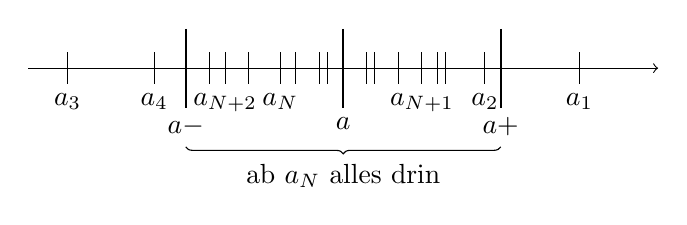
\begin{tikzpicture}
        \draw[->] (-4,0) -- (4,0);
        \draw[thick] (0,0.5) -- (0,-0.5) node[below] {$a$}
        (-2,0.5) -- (-2,-0.5) node[below] {$a-\eps$}
        (2,0.5) -- (2,-0.5) node[below] {$a+\eps$};
        \foreach \x [count=\n] in {3, 1.8, -3.5, -2.4}
        \draw (\x,0.2) -- (\x,-0.2) node[below] {$a_{\n}$};
        \draw (-0.8,0.2) -- (-0.8,-0.2) node[below] {$a_N$};
        \foreach \x [count=\n] in {1, -1.5}
        \draw (\x,0.2) -- (\x,-0.2) node[below] {$a_{N+\n}$};
        \foreach \x in {0.3, 0.7, 0.4, 1.2, 1.3, -0.3, -0.2, -0.6, -1.2, -1.7}
        \draw (\x,0.2) -- (\x,-0.2);
        \draw[decorate, decoration={brace, mirror}] (-2,-1) -- (2,-1) node[midway, below, yshift=-0.1cm] {ab $a_N$ alles drin};
    \end{tikzpicture}
    \caption{Visualisierung des Konvergenzbegriffs.}\label{fig:convergence}
\end{figure}

\begin{definition}[Nullfolge]
    Eine Folge heißt \emph{Nullfolge}, falls sie gegen~0 konvergiert.
\end{definition}

\begin{theorem}
    Der Grenzwert einer konvergenten Folge ist eindeutig.
\end{theorem}

\begin{proof}[Beweis durch Widerspruch]
    Die Annahme ist, dass es zwei Grenzwerte $a$ und~$b \neq a$ gibt. Um die Annahme zu widerlegen, reicht es, ein~$\eps$ als Gegenbeispiel zu finden. Dafür setzen wir $\eps = \frac{1}{2}\abs{a-b} > 0$. Also existieren $N_a$~und~$N_b$ mit $\abs{a_n - a} < \eps$ für alle~$n \geq N_a$, und $\abs{a_n - b} < \eps$ für alle~$n \geq N_b$. Wir setzen nun $N \coloneqq \max(N_a, N_b)$, d.\,h., dass mit der Dreiecksungleichung für alle~$n \geq N$ dann
    \begin{equation*}
        \abs{a-b} = \abs{(a-a_n) + (a_n-b)} \leq \abs{a-a_n} + \abs{a_n-b} < \eps + \eps = 2 \eps = \abs{a-b}
    \end{equation*}
    gilt, was aber $\abs{a-b} < \abs{a-b}$ bedeuten würde. Ein Widerspruch.
\end{proof}

Alternativ hätten wir auch $\eps = \abs{a-b}/4$ wählen können, was dann zum Widerspruch $\abs{a-b} < \frac{1}{2}\abs{a-b}$ führt. Ähnlich sind weitere Variationen des Beweises möglich.

\begin{example}\leavevmode
    \begin{enumerate}
        \item Die konstante Folge mit $a_n \coloneqq b$ für alle~$n$ konvergiert gegen~$b$.
        \item Die alternierende Folge $\paren*{(-1)^n}_{n \in \N_0} = (1, -1, 1, -1, \dots)$ divergiert.
              \begin{proof}
                  Wenn die Folge doch gegen~$a \in \R$ konvergiert, können wir~$\eps = 1$ wählen, wozu es ein~$N$ gibt mit $\abs{a_n-a} < 1$ und natürlich auch $\abs{a_{n+1}-a} < 1$ für alle~$n \geq N$. Daraus folgt $2 > \abs{a_n-a} + \abs{a-a_{n+1}} \geq \abs{(a_n-a) + (a-a_{n+1})} = \abs{a_n-a_{n+1}} = 2$, Widerspruch.
              \end{proof}
        \item $(1/n)_{n \in \N}$ ist eine Nullfolge.
              \begin{proof}
                  Für jedes~$\eps > 0$ gibt es ein~$N \in \N$ mit $N > 1/\eps$ (archimedisches Axiom, \cref{arch:inverse}). Daher gilt für alle~$n \geq N$: $\abs{1/n-0} \leq 1/N < \eps$, also ist 0~der Grenzwert.
              \end{proof}
        \item $\paren*{2^n}_n$ und die Fibonacci-Folge sind divergent, da beide unbeschränkt sind.
        \item Wir betrachten die Folge~$\paren*{x^n}_{n\in\N}$ mit~$x \in \R$. Dann gibt es vier Fälle:
              \begin{enumerate}
                  \item $x = 1$ liefert eine konstante Folge, die gegen~1 konvergiert.
                  \item $x = -1$ liefert die alternierende Folge, die divergiert.
                  \item $\abs{x} > 1$ liefert eine unbeschränkte Folge, die divergiert.
                  \item $\abs{x} < 1$ ist eine Nullfolge.
                        \begin{proof}[Beweis zu~(d)]
                            Aufgrund \cref{thm:archimedesbernoulli} gibt es für jedes~$\eps > 0$ ein~$N \in \N$, für das $\abs{x}^N < \eps$ gilt. Daher ist $\abs{x^n-0} = \abs{x}^n \leq \abs{x}^N < \eps$.
                        \end{proof}
              \end{enumerate}
    \end{enumerate}
\end{example}

\begin{definition}[beschränkte Folge]
    $(a_n)_{n\in\N}$ heißt \emph{beschränkt}, falls es ein~$K \in \R$ gibt, sodass $\abs{a_n} \leq K$ für alle~$n \in \N$ gilt. Analog ist $(a_n)$ \emph{nach oben beschränkt}, falls es ein~$K$ gibt, sodass $a_n \leq K$ für alle~$n$ ist.
\end{definition}

\begin{example}
    $\paren*{x^n}_n$ mit~$\abs{x} > 1$ ist unbeschränkt, weil es nach \cref{thm:archimedesbernoulli} ein~$K \in \R$ gibt, sodass $\abs{x}^n > K$ für alle~$n$ ist.
\end{example}

\begin{theorem}\label{thm:bound}
    Jede konvergente Folge ist beschränkt.
\end{theorem}

\begin{proof}
    Wir nehmen an, dass $(a_n)$ gegen~$a$ konvergiert. Wählen wir~$\eps = 1$, so gibt es ein~$N$ mit $\abs{a_n - a} < 1$ für alle~$n \geq N$, also gilt nach der Dreiecksungleichung
    \begin{equation*}
        \abs{a_n} \leq \abs{a_n-a} + \abs{a} < 1 + \abs{a}.
    \end{equation*}
    Setzen wir $K = \max\mset{\abs{a_1}, \abs{a_2}, \dots, \abs{a_{n-1}}, 1+\abs{a}}$, gilt dann $\abs{a_n} \leq K$ für alle~$n \in \N$.
\end{proof}

\subsection{Grenzwertsätze}

\begin{theorem}[Summe/Differenz und Produkt konvergenter Folgen]
    Sind $(a_n)$~und~$(b_n)$ konvergent, so konvergiert auch ihre Summe~$(a_n + b_n)$ und ihr Produkt~$(a_n b_n)$ und es gilt
    \begin{equation*}
        \lim_{n\to\infty} (a_n + b_n) = \paren*{\lim_{n\to\infty} a_n} + \paren*{\lim_{n\to\infty} b_n}, \qquad \lim_{n\to\infty} (a_n b_n) = \paren*{\lim_{n\to\infty} a_n} \paren*{\lim_{n\to\infty} b_n}.
    \end{equation*}
    Die Subtraktion folgt aus $(\lim_{n\to\infty} a_n) + (\lim_{n\to\infty} (-1)) (\lim_{n\to\infty} b_n)$
\end{theorem}

\begin{proof}
    Zuerst zur Summenfolge: Es konvergieren $a_n \to a$ und $b_n \to b$ für~$n \to \infty$. Nach Voraussetzung gibt es zu jedem~$\eps > 0$ Zahlen $N_a, N_b \in \N$, sodass $\abs{a_n-a} < \frac{1}{2}\eps$ für alle~$n \geq N_a$, und $\abs{a_n-b} < \frac{1}{2}\eps$ für alle~$n \geq N_b$ gilt. Setzen wir nun $N \coloneqq \max(N_a, N_b)$, erhalten wir mit der Dreiecksungleichung für alle~$n \geq N$
    \begin{equation*}
        \abs{(a_n+b_n) - (a+b)} \leq \abs{a_n-a} + \abs{b_n-b} < \frac{\eps}{2} + \frac{\eps}{2} = \eps.
    \end{equation*}
    (Alternativ können wir auch $\abs{a_n-a} < \eps$ und $\abs{b_n-b} < \eps$ nehmen, woraus $\abs{(a_n+b_n) - (a+b)} < 2\eps$ folgt.)

    Jetzt zur Produktfolge: Da $(a_n)$~konvergiert, existiert eine obere Schranke~$K > 0$, sodass $\abs{a_n} < K$ für alle~$n$ (\cref{thm:bound}). Nach Voraussetzung gibt es für jedes~$\eps > 0$ Zahlen $N_a, N_b \in \N$, sodass $\abs{a_n-a} < \eps$ für alle~$n \geq N_a$ und $\abs{b_n-b} < \eps$ für alle~$n \geq N_b$ gilt. Mit der Dreiecksungleichung folgt daraus
    \begin{equation*}
        \abs{a_nb_n - ab} = \abs{a_nb_n - a_nb + a_nb - ab} = \abs{a_n(b_n-b) + (a_n-a)b} \leq \abs{a_n} \cdot \abs{b_n-b} + \abs{a_n-a} \cdot \abs{b} < K\eps + \eps\abs{b} = \eps (K+\abs{b}).
    \end{equation*}
    Da $K+\abs{b}$ eine Konstante ist und $\eps$~beliebig klein werden kann, kann auch $\eps (K+\abs{b})$ beliebig klein werden.

    Nun nochmals zurück, um den Beweis besser aufzuschreiben: Wir wählen nun~$N$ so, dass für alle~$n \geq N$ gilt:
    \begin{equation*}
        \abs{a_n-a} < \frac{\eps}{K+\abs{b}},\;\; \abs{b_n-b} < \frac{\eps}{K+\abs{b}} \implies \dots \implies \abs{a_nb_n - ab} < \frac{\eps}{K+\abs{b}} (K+\abs{b}) = \eps. \qedhere
    \end{equation*}
\end{proof}

\begin{example}
    Die geometrische Reihe konvergiert für~$x \in \R$ mit~$\abs{x} < 1$ gegen
    \begin{equation*}
        \lim_{n\to\infty} \frac{1-x^{n+1}}{1-x} = \frac{1}{1-x} - \frac{1}{1-x} \lim_{n\to\infty} x^{n+1} = \frac{1}{1-x}.
    \end{equation*}
\end{example}

Bevor wir die Division zweier konvergenter Folgen betrachten, brauchen wir noch eine alternative Form der Dreiecksungleichung.

\begin{lemma}[umgekehrte Dreiecksungleichung]\label{lem:reversetriangleineq}
    Für alle $x, y \in \R$ gilt
    \begin{equation*}
        \abs{x - y} \geq \abs{x} - \abs{y}.
    \end{equation*}
\end{lemma}

\begin{proof}
    Für alle reellen Zahlen~$a, b$ gilt gemäß der Dreiecksungleichung $\abs{a} \geq \abs{a+b} - \abs{b}$. Nach einsetzen von~$a = x+z$ und~$b = -z$ haben wir $\abs{x+z} \geq \abs{x} - \abs{z}$ (auch eine nützliche Ungleichung). Setzen wir nun~$z = -y$, erhalten wir das Lemma.\footnote{Die "`Mutter"' aller Dreiecksungleichungen ist auch sehr nützlich: $\abs{\abs{x} - \abs{y}} \leq \abs{x \pm y} \leq \abs{x} + \abs{y}$. Das haben wir in der Übung bewiesen.}
\end{proof}

\begin{theorem}[Quotient konvergenter Folgen]
    Seien $(a_n)$~und~$(b_n)$ konvergente Folgen mit $\lim_{n\to\infty} b_n = b \neq 0$. Dann existiert ein~$k \in \N$ mit~$b_n \neq 0$ für alle~$n \geq k$, und die Folge $(a_n/b_n)_{n \geq k}$ konvergiert mit dem Limes
    \begin{equation*}
        \lim_{n\to\infty} \frac{a_n}{b_n} = \frac{\lim_{n\to\infty} a_n}{\lim_{n\to\infty} b_n}
    \end{equation*}
\end{theorem}

\begin{remark}
    Die Existenz des oben genannten~$k$ ist gesichert, weil wir ein~$0 < \eps < \abs{b}$ wählen können, und es dafür ein~$k \in \N$ geben muss mit $\abs{b_n - b} < \eps < \abs{b}$ für alle~$n \geq k$. Diese~$b_n$ sind dann entweder alle positiv oder negativ, je nachdem ob~$b$ positiv oder negativ ist. Mit anderen Worten: Wir warten so lange, bis~$k$ hinreichend groß ist und die~$b_n$ in der Nähe von~$b$ liegen, also ungleich Null sind.
\end{remark}

\begin{proof}
    Wir versuchen den Sachverhalt auf bekanntes zurückzuführen: Konvergiert $(1/b_n)_{n \geq k}$ gegen~$1/b$, dann folgt der Rest aus dem vorherigen Satz über Produktfolgen: $a_n/b_n = a \cdot (1/b_n)$.

    Nun zur Konvergenz von~$(1/b_n)$: Nach Voraussetzung ist~$b \neq 0$. Mit~$\eps = \frac{1}{2}\abs{b}$ folgt, dass ein~$N \geq k$ existiert, sodass
    \begin{align*}
        \abs{b_n} \geq \abs{b} - \abs{b_n-b} > \abs{b} - \eps = \frac{1}{2}\abs{b}
    \end{align*}
    für alle~$n \geq N$. Dabei folgte die erste Abschätzung aus \cref{lem:reversetriangleineq}, die zweite aus der Konvergenz von $b_n \to b$. Ferner gibt es zu jedem~$\eps > 0$ ein~$N' \in \N$, sodass $\abs{b_n-b} < \frac{1}{2} \eps \abs{b}^2$ für alle~$n \geq N'$ gilt. Daher haben wir für alle~$n \geq \max(N, N')$
    \begin{equation*}
        \abs*{\frac{1}{b_n} - \frac{1}{b}} = \abs{b_n-b} \cdot \frac{1}{\abs{b_n}} \cdot \frac{1}{\abs{b}} < \frac{\eps \abs{b}^2}{2} \cdot \frac{2}{\abs{b}} \cdot \frac{1}{\abs{b}} = \eps. \qedhere
    \end{equation*}
\end{proof}

Alternativ hätten wir für die letzte Abschätzung auch $\abs{1/b_n - 1/b} < \eps (\abs{b} - \eps) / \abs{b}$ erhalten können.\footnote{Noch ein hilfreicher Grenzwertsatz ist die \emph{$k$"~te Wurzel einer konvergenten Folge}: Ist $a_n \to a$ nicht-negativ, so gilt $\sqrt[k]{a_n} \to \sqrt[k]{a}$ für alle~$k \in \N$. \emph{Beweis}: Generell gilt für $x \geq y \geq 0$ mit dem binomischen Lehrsatz und anschließendem Weglassen von positiven Summanden: $x^k = (y+(x-y))^k \geq y^k + (x-y)^k \iff x^k-y^k \geq (x-y)^k$. Um den Fall $x \leq y$ zu beachten, können wir Betragsstriche setzen: $\abs{x^k-y^k} \geq \abs{x-y}^k$. Ersetzen wir $x = \sqrt[k]{a_n}$ und $y = \sqrt[k]{a}$, erhalten wir nach umstellen $\abs{\sqrt[k]{a_n}-\sqrt[k]{a}} \leq \sqrt[k]{\abs{a_n-a}}$. Mit $\abs{a_n-a} \leq \eps^k$ folgt die Behauptung.}

\begin{example}
    Um den Grenzwert rationaler Funktionen in~$n$ können wir bestimmen, indem wir den größten Exponenten aus Zähler und Nenner ausklammern und dann kürzen. Viele Summanden reduzieren sich dann zu Nullfolgen.
    \begin{equation*}
        \lim_{n\to\infty} \frac{7n^2 + 13n + 24}{n^2 - 2n - 8} = \lim_{n\to\infty} \frac{7 + 13/n + 24/n^2}{1 - 2/n - 8/n^2} = \frac{\lim_{n\to\infty} \paren*{7 + 13/n + 24/n^2}}{\lim_{n\to\infty} \paren*{1 - 2/n - 8/n^2}} = \frac{7 + 0 + 0}{1 - 0 - 0} = 7.
    \end{equation*}
    Beachte, dass der Nenner $1 - 2/n - 8/n^2 \neq 0$ für natürliche~$n$ ist.
\end{example}

\begin{theorem}[Ordnungserhaltung konvergenter Folgen]\label{thm:sequence:monotony}
    Falls $(a_n)$ und~$(b_n)$ konvergent sind, gilt dann
    \begin{equation*}
        \forall n\colon a_n \leq b_n \implies \lim_{n\to\infty} a_n \leq \lim_{n\to\infty} b_n.
    \end{equation*}
\end{theorem}

\begin{proof}
    Wir betrachten die Folge $c_n \coloneqq b_n - a_n \geq 0$. Wäre $c \coloneqq \lim_{n\to\infty} c_n < 0$, so folgt aus der Konvergenz, dass es ein~$\eps = -c > 0$ gibt, sodass $\abs{c_n-c} < \eps = -c$ gilt. Weil $c_n \geq 0 > c$, können wir die Betragsstriche weglassen und erhalten $c_n-c < -c \iff c_n < 0$, ein Widerspruch.\footnote{Der Dozent gab einen (eher intuitiven) Beweis, dass $c_n$~für große~$n$ in eine $\frac{1}{2}\abs{c}$"~Umgebung kommen muss, also $c_n \leq \frac{1}{2}c < 0$.}
\end{proof}

\begin{corollary}\label{cor:sequence:monotony}
    Falls $K \leq a_n \leq L$ für alle~$n \in \N$ ist, gilt dann $K \leq \lim_{n\to\infty} a_n \leq L$.
\end{corollary}

Das Korollar erhalten wir durch Abschätzung einer Folge durch konstante Folgen $(K)_n$~und~$(L)_n$ von oben und unten.

\emph{Achtung}: \cref{thm:sequence:monotony,cor:sequence:monotony} gelten \underline{nicht} mit~$<$ an Stelle von~$\leq$. \emph{Gegenbeispiel}: Es gilt $a_n = 1/n > 0$ für alle~$n \in \N$, aber $\lim_{n\to\infty} a_n = 0$.

\lecturesep{25.~Oktober 2021}

\section{Das Vollständigkeitsaxiom}

\subsection{Motivation}

Mit den bisherigen Axiomen können wir aus den natürlichen Zahlen~$\N = \mset{1, 2, 3, \dots}$ nacheinander die uns bekannten Zahlenbereiche konstruieren.

Die Menge der ganzen Zahlen~$\Z = \N \cup \mset{0} \cup -\N$ lässt sich dann als Menge der Äquivalenzklassen~$\Z = \mset{m-n : m, n \in \N} / \sim$ mit der Äquivalenzrelation $m-n \sim m'-n'$, falls $m+n' = m'+n$, definieren.\footnote{Eine kurze (unsaubere) Definition von Äquivalenzrelationen: Eine \emph{Äquivalenzrelation}~$\sim$ über eine Menge~$M$ ist eine Relation, für die noch zusätzlich $a \sim a$ (\emph{Reflexivität}), $a \sim b \iff b \sim a$ (\emph{Symmetrie}) und $(a \sim b \wedge b \sim c) \implies a \sim c$ (\emph{Transitivität}) für alle~$a, b, c \in M$ erfüllt. Intuitiv sind das auch Eigenschaften des Begriffs "`Äquivalenz"'. Eine \emph{Äquivalenzklasse} ist nun die Menge aller Elemente, die zueinander äquivalent sind, also $[a]_\sim \coloneqq \mset{b \in M : a \sim b}$. Die Menge aller \emph{Äquivalenzklassen}~$M/{\sim}$ ist $M/{\sim} = \mset{[a]_\sim : a \in M}$.} Die Äquivalenzrelation sagt, wann zwei Darstellungen $m-n$ und $m'-n'$ dieselbe Zahl repräsentieren, nämlich wenn dieselbe Differenz rauskommt. $\Z$~ist nun die Menge aller dieser Differenzen.

Ähnlich lässt sich die Menge der rationalen Zahlen~$\Q$ definieren als die Menge der Äquivalenzklassen~$\Q = \mset{m/n : m \in \Z, n \in \Z} / \sim$ mit der Äquivalenzrelation $m/n \sim m'/n'$, falls $mn' = m'n$ gilt (Brüche bleiben nach Kürzen bzw.\ Erweitern dieselben). $\Q$~ist nun die Menge aller dieser Quotienten.

$\Q$~und~$\R$ sind nun beides archimedisch angeordnete Körper. Aber wir wissen, dass $\Q$~nicht "`vollständig"' ist, es weist "`Löcher"'\footnote{"`Löcher"' ist ein irreführendes Wort. Genau wie~$\R$ ist auch~$\Q$ "`unendlich dicht"' (zwischen zwei "`Zahlen"' gibt es stets eine "`dazwischen"'). Der Unterschied zwischen den beiden liegt vielmehr in der \emph{Abzählbarkeit}.} auf. Es gibt nämlich "`Zahlen"', die nicht in~$\Q$ enthalten sind, wie z.\,B\ Wurzeln wie~$\sqrt{2} \notin \Q$. Denn wäre $\sqrt{2} = m/n \in \Q$, dann ist $2m^2 = n^2$. In der Primfaktorzerlegung der linken Seite steht eine Zweierpotenz mit ungeradem Exponenten, während auf der Zerlegung der rechten Seite ein gerader Exponent auftritt, was unmöglich ist.

Das Ziel ist, die Löcher von~$\Q$ zu stopfen. Dazu gibt es verschiedene Ansätze:
\begin{enumerate}
    \item \emph{\textsc{Cauchy}-Folgen},
    \item \emph{Intervallschachtelungen} und
    \item \emph{\textsc{Dedekindsche} Schnitte}, was in der Übung erfolgt.
\end{enumerate}

\subsection{Cauchy-Folgen}

\begin{definition}[\textsc{Cauchy}-Folge]\label{def:cauchysequence}
    Eine Folge~$(a_n)_{n \in \N}$ reeller Zahlen heißt \emph{\textsc{Cauchy}-Folge}, wenn es für jedes~$\eps > 0$ ein~$N \in \N$ gibt, für das $\abs{a_n - a_n} < \eps$ für alle $m, n \geq N$ gilt.
\end{definition}

\begin{remark}\leavevmode
    \begin{enumerate}
        \item Die Idee hier ist, den Begriff der Konvergenz zu definieren, ohne den Limes zu verwenden. Anstatt zu sagen, dass Folgenglieder sich einem Grenzwert annähern, können Folgenglieder sich gegenseitig annähern. Diese Definition ist hilfreich, denn nicht für alle Folgen ist der Grenzwert gemäß den Grenzwertsätzen, Null"~ und konstanten Folgen definiert, aber die Cauchy-Folge, wie z.\,B.\ für die rekursive Folge $a_{n+1} = 1 + 1/a_n$.
        \item Es reicht \underline{nicht}, hier nur $\abs{a_n - a_{n+1}} < \eps$ für zwei aufeinanderfolgende Glieder zu verifizieren. \emph{Beispiel}: Für die \emph{harmonische Reihe} $a_n \coloneqq \sum_{k=1}^n 1/k$ gilt $\abs{a_n - a_{n+1}} = 1/(n+1) < \eps$ für hinreichend große~$n$ aufgrund des archimedischen Axioms. Trotzdem divergiert die Reihe.\footnote{Das kann man zeigen, indem man geschickt abschätzt und somit zeigt, dass die Folge nach oben unbeschränkt ist:
                  \begin{equation*}
                      1 + \frac{1}{2} + \paren*{\frac{1}{3} + \frac{1}{4}} + \paren*{\frac{1}{5} + \frac{1}{6} + \frac{1}{7} + \frac{1}{8}} + \dots > 1 + \frac{1}{2} + \paren*{\frac{1}{4} + \frac{1}{4}} + \paren*{\frac{1}{8} + \frac{1}{8} + \frac{1}{8} + \frac{1}{8}} + \dots = 1 + \frac{1}{2} + \frac{1}{2} + \frac{1}{2} + \cdots
                  \end{equation*}}
    \end{enumerate}
\end{remark}

\begin{theorem}\label{thm:convergencecauchy}
    Jede konvergente Folge reeller Zahlen ist eine Cauchy-Folge.
\end{theorem}

\begin{proof}
    Angenommen $(a_n)$~konvergiert gegen~$a \in \R$. Dann gibt es für jedes~$\eps > 0$ ein~$N \in \N$, sodass $\abs{a_n - a} < \frac{1}{2}\eps$ für alle~$n \geq N$ gilt. Daraus folgt wegen der Dreiecksungleichung $\abs{a_n - a_m} \leq \abs{a_n - a} + \abs{a - a_m} < \eps$ für alle~$n, m \geq N$.
\end{proof}

\subsection{Vollständigkeitsaxiom (Vollständigkeit in \texorpdfstring{$\R$}{R})}\label{subsec:completeness}

Mit \cref{thm:convergencecauchy} haben wir gezeigt, dass jede konvergente Folge eine Cauchy-Folge ist, also Cauchy-Folgen unserer Idee von Konvergenz entsprechen. Die Umkehrung müssen wir aber als Axiom voraussetzen.

\begin{axiom}[Vollständigkeitsaxiom]
    Jede Cauchy-Folge reeller Zahlen konvergiert in~$\R$.
\end{axiom}

\begin{example}
    Wir betrachten die Dezimalbruchentwicklung einer reellen Zahl~$x \in \R$ mit~$x \geq 0$. Setze dafür~$x_n \coloneqq 10^{-n} \floor*{10^n x}$ als die Zahl, die dadurch entsteht, indem wir nach der $n$"~ten Nachkommastelle alle Ziffern abschneiden. $(x_n)$~liefert eine Cauchy-Folge in~$\Q$, denn $\abs{x_n - x_m} \leq 10^{-N}$ für alle~$n, m \geq N$. Die Folge~$(x_n)$ konvergiert in~$\Q$ genau dann, wenn $x \in \Q$ ist.
\end{example}

Mit dem obigen Beispiel sehen wir, wie wir aus~$\Q$ mithilfe von rationalen Cauchy-Folgen jede reelle Zahl konstruieren können: Sei~$\hat{\Q} \coloneqq \mset{(a_n) : \text{Cauchy-Folgen in }\Q}$ mit der Äquivalenzrelation $((a_n) \sim (b_n)) \coloniff ((a_n - b_n) \text{ ist Nullfolge})$. Dann ist $\R \coloneqq \hat{\Q}/{\sim}$, wobei $\Q$~in~$\R$ eingebettet wird, indem wir jedes~$q \in \Q$ mit der konstanten Folge $(q, q, q, \dots)$ identifizieren.

\subsection{Intervallschachtelung}

\begin{definition}[Intervall]\label{def:interval}
    Für $a, b \in \R$ mit~$a \leq b$ sind
    \begin{itemize}
        \item $[a, b] \coloneqq \mset{x \in \R : a \leq x \leq b}$ das \emph{abgeschlossen Intervall},
        \item $(a, b) \coloneqq \mset{x \in \R : a < x < b}$ das \emph{offene Intervall} und
        \item $[a, b)$~sowie~$(a, b]$ \emph{halboffene Intervalle}.
    \end{itemize}

    $a$~und~$b$ heißen \emph{Randpunkte} der jeweiligen Intervalle. $\abs{b-a}$~heißt \emph{Länge} des Intervalls, kurz $\diam([a, b])$.
\end{definition}

\begin{definition}[Intervallschatelung]
    Eine \emph{Intervallschachtelung} ist eine Folge~$(I_n)_{n \in \N}$ von \emph{abgeschlossenen} Intervallen~$I_n = \abs{a_n, b_n}$ mit
    \begin{enumerate}
        \item $I_{n+1} \subset I_n$ für alle~$n \in \N$, und
        \item $\lim_{n\to\infty} \diam(I_n) = 0$.
    \end{enumerate}
\end{definition}

Die Idee ist, dass wir einen Grenzwert von oben und unten eingrenzen, und diese Intervalle immer kleiner werden lassen, bis das Intervall dem Grenzwert "`entspricht"'.

\begin{theorem}[Intervallschachtelungsprinzip]
    Für jede Intervallschachtelung~$(I_n)_{n\to\infty}$ in~$\R$ gibt es eine reelle Zahl $x \in \bigcap_{n\in\N} I_n$. Oder mit anderen Worten: Es gibt ein~$x \in \R$, sodass $x \in I_n$ für alle~$n \in \N$ gilt.\footnote{Dieser Satz ist äquivalent zum \emph{Einschnürungssatz}, bewiesen durch \textsc{Gauß}: Ist $a_n \leq c_n \leq b_n$ für alle~$n \in \N$ und $\lim a_n = \lim b_n$, so folgt daraus $\lim c_n = \lim a_n = \lim b_n$. Die Aussage ist auch ein Korollar von \cref{thm:sequence:monotony}.}
\end{theorem}

Die Beweisidee ist, die linken und rechten Randpunkte der Intervalle als zwei monotone Folgen aufzufassen, wobei die linken Randpunkte eine Cauchy-Folge~$a_n \to a$ implizieren. Nun können wir aber~$a$ zwischen beiden Folgen "`schachteln"'.

\begin{proof}
    Gegeben sei die Intervallschachtelung $(I_n)_n$ mit~$I_n = [a_n, b_n]$, $(a_n)_n$ eine nicht fallende Folge, $(b_n)_n$ eine nicht wachsende Folge und $\diam(I_n) = (b_n - a_n)_n$ eine Nullfolge.

    Dann ist $(a_n)$ eine Cauchy-Folge, denn aufgrund der Nullfolge gibt es für jedes~$\eps > 0$ ein~$N \in \N$ mit $b_N - a_N = \abs{(b_N - a_N) - 0} < \eps$. Wegen der Monotonie gilt~$a_N \leq a_n$ und
    $a_m \leq b_n \leq b_N$ für alle $m, n \geq N$. Daher ist $\abs{a_n - a_m} \leq b_N - a_N < \eps$, weshalb $(a_n)$~eine Cauchy-Folge ist. Das bedeutet aber auch, dass nach dem Vollständigkeitsaxiom ein Grenzwert $a_n \to a \in \R$ für~$n \to \infty$ existiert.

    Da die Ordnungsrelation~$\leq$ unter Konvergenz erhalten bleibt (\cref{cor:sequence:monotony}), gilt $a_N \leq a \leq b_N$ für alle~$N \in \N$, woraus auch $a \in \bigcap_{N \in \N} I_N$ folgt.
\end{proof}

\begin{remark}\leavevmode
    \begin{enumerate}
        \item Das Intervallschachtelungsprinzip gilt \underline{nicht} für offene Intervalle. Z.\,B.\ gilt $\bigcap_{n\in\N} \paren*{0, n^{-1}} = \varnothing$.
        \item Die Zahl~$x \in \bigcap_{n\in\N} I_n$ bei Schachtelung abgeschlossener Intervalle ist eindeutig. Für jedes weitere $x' \in \bigcap I_n$ würde nämlich $\abs{x-x'} \leq \diam(I_n) \to 0$ für~$n \to \infty$ gelten, also $\abs{x-x'} = 0$ und damit~$x = x'$.\footnote{Eine dritte Bemerkung: Als Nebenprodukt folgt aus dem Beweis, dass $\bigcap_n I_n$ auch Grenzwert von $(a_n)$ und~$(b_n)$ ist.}
    \end{enumerate}
\end{remark}

Tatsächlich gilt für alle archimedisch angeordneten Körper

\begin{theorem}
    Das Vollständigkeitsaxiom ist äquivalent zum Intervallschachtelungsprinzip.
\end{theorem}

\begin{proof}
    Die Hinrichtung haben wir mit dem Intervallschachtelungsprinzip schon bewiesen. Es bleibt noch die Rückrichtung zu zeigen.

    Sei $(a_n)$~eine Cauchy-Folge, weshalb für alle~$k \in \N$ ein~$N_k \in \N$ existiert, sodass $\abs{a_n - a_m} < \eps = 2^{-k}$ für alle $m, n \geq N_k$ gilt.

    Wir definieren die Intervalle
    \begin{equation*}
        I_k \coloneqq \mbrack*{a_{N_k} - 2^{-k+1}, a_{N_k} + 2^{-k+1}}
    \end{equation*}
    für alle~$k \in \N$. Nun ist die Folge~$(I_k)_{k\in\N}$ eine Intervallschachtelung aus den folgenden Gründen: 1.~Die~$I_k$ sind abgeschlossen. 2.~Des Weiteren ist~$I_{k+1} \subset I_k$, denn für alle~$x \in I_{k+1}$ gelten $\abs*{x - a_{N_{k+1}}} \leq 2^{-k}$, weil $a_{N_{k+1}}$ der Mittelpunkt von~$I_{k+1}$ ist, und $\abs*{a_{N_{k+1}} - a_{N_k}} < 2^{-k}$ wegen des Cauchy-Kriteriums. Deshalb folgt
    \begin{equation*}
        \abs*{x - a_{N_k}} \leq \abs*{x - a_{N_{k+1}}} + \abs*{a_{N_{k+1}} - a_{N_k}} < 2^{-k} + 2^{-k} = 2^{-k+1},
    \end{equation*}
    also $x \in I_k$. 3.~Ferner ist offensichtlich $\diam(I_k) \to 0$ für~$k \to \infty$. Damit ist~$(I_k)_{k\in\N}$ eine Intervallschachtelung.

    Nach dem Intervallschachtelungsprinzip gibt es ein~$x \in \bigcap_{k\in\N} I_k$ (also ein~$x$ in allen Intervallen), wofür stets $\abs*{x - a_{N_k}} \leq 2^{-k+1}$ gilt ($a_{N_k}$~ist der Mittelpunkt von
    $I_k$). Damit und mit $\abs*{a_{N_k}-a_n} < 2^{-k}$ (Cauchy-Kriterium) erhalten wir
    \begin{equation*}
        \abs{x - a_n} \leq \abs*{x - a_{N_k}} + \abs*{a_{N_k} - a_n} < 2^{-k+1} + 2^{-k} = 3 \cdot 2^{-k} = \eps
    \end{equation*}
    für alle~$k \in \N$, weshalb $a_n \to x$ für~$n \to \infty$.
\end{proof}

In diesem Beweis nahmen wir eine Cauchy-Folge~$(a_n)$ und konstruierten darum eine Intervallschachtelung symmetrisch um~$a_n$, wobei sich die Länge der Intervalle sukzessive halbiert. Diese Intervallschachtelung umschließt ein~$x$, sodass auch die Cauchy-Folge gegen~$x$ konvergiert, was das Vollständigkeitsaxiom ist.

\begin{example}[für Intervallschachtelungen]\leavevmode
    \begin{enumerate}
        \item Für alle~$x \in \R$ sei $I_k = \mbrack*{x-k^{-1}, x+k^{-1}}$. Dann gilt $\mset{x} = \bigcap_{k\in\N} I_k$. Ähnliche Beispiele wären $I_k = \mbrack*{x, x+2^{-k}}$, etc.
        \item Seien $f_n$~und~$F_n$ die Flächen der den Einheitskreis einbeschriebenen bzw.\ umschriebenen $n$"~Ecke. Seien $I_k \coloneqq \mbrack*{f_{3\cdot2^{-k}}, F_{3\cdot2^{-k}}}$, wobei offensichtlich $I_{k+1} \subset I_k$ gilt. Dann approximieren die~$I_k$ die Kreiszahl~$\pi$: $\bigcap_{k\in\N} I_k = \mset{\pi}$ durch die Folge von Dreiecken, Sechsecken, Zwölfecken, etc.

              Hierbei ist $f_6 = \frac{3}{2} \sqrt{3}$ und $F_6 = 2 \sqrt{3}$. Schon \textsc{Archimedes} wusste $f_{192} = 3 + 10/71$ und $F_{192} = 3 + 10/70$.

              \begin{figure}
                  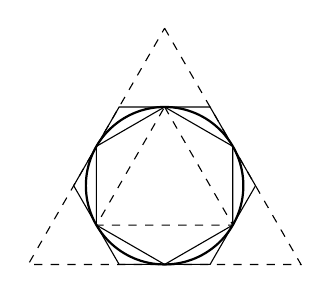
\begin{tikzpicture}
                      \draw[thick] (0,0) circle [radius=1];
                      \draw[dashed] (90:1) -- (-30:1) -- (-150:1) -- cycle;
                      \draw (90:1) -- (30:1) -- (-30:1) -- (-90:1) -- (-150:1) -- (150:1) -- cycle;
                      \draw[dashed] (90:2) -- (-30:2) -- (-150:2) -- cycle;
                      \draw (120:1.1547) -- (60:1.1547) -- (0:1.1547) -- (-60:1.1547) -- (-120:1.1547) -- (180:1.1547) -- cycle;
                  \end{tikzpicture}
                  \caption{Erste Annäherung der Kreisfläche durch Dreiecke $f_3, F_3$ und Sechsecke $f_6, F_6$.}
              \end{figure}
    \end{enumerate}
\end{example}

\subsubsection{Wurzeln}

\begin{theorem}[Existenz der Wurzeln]
    Für alle~$x > 0$ und für alle~$k \in \N$ gibt es genau ein~$y > 0$ mit~$y^k = x$.
\end{theorem}

\begin{notation}
    $y = \sqrt[k]{x} = x^{1/k}$ bezeichnet die \emph{$k$"~te Wurzel} von~$x$.
\end{notation}

\begin{proof}
    Wir betrachten zunächst den Fall~$x > 1$. Hierfür definieren wir eine Intervallschachtelung $I_n = [a_n, b_n]$ rekursiv mit $a_1 = 1$, $b_1 = x$, und $c_n = \frac{1}{2}(a_n + b_n)$. Dann ist $I_{n+1} = [a_{n+1}, b_{n+1}]$ mit
    \begin{equation*}
        \begin{cases}
            a_{n+1} \coloneqq a_n,\; b_{n+1} \coloneqq c_n, & \text{falls } x \leq c_n^k, \\
            a_{n+1} \coloneqq c_n,\; b_{n+1} \coloneqq b_n, & \text{falls } x > c_n^k.
        \end{cases}
    \end{equation*}
    $(I_n)$~erfüllt alle Bedingungen einer Intervallschachtelung: Die $I_n$ sind abgeschlossen, es gilt~$I_{n+1} \subset I_n$ und $\diam(I_{n+1}) = \frac{1}{2} \diam(I_n) = 2^{-n} (x-1) \to 0$ für alle~$n \in \N$. Deshalb folgt aus dem Intervallschachtelungsprinzip, dass es ein~$y \in \bigcap_{n\in\N} I_n$ gibt.

    Nun betrachten wir die Intervalle~$J_n = \mbrack*{a_n^k, b_n^k}$. Auch~$(J_n)$ ist eine Intervallschachtelung: Die $J_n$ sind abgeschlossen, es gilt $J_{n+1} \subset J_n$ und wir haben
    \begin{equation*}
        \diam(J_n) = b_n^k - a_n^k = (b_n - a_n) \paren*{b_n^{k-1} + a_n b_n^{k-2} + \dots + a_n^{k-2} b_n + a_n^{k-1}} \leq \diam(I_n) \cdot k x^{k-1} \to 0
    \end{equation*}
    für~$n \to \infty$. Die letzte Abschätzung gilt wegen $x \geq b_n \geq a_n \iff x^{k-1} \geq b_n^{k-1} \geq a_n^{k-1}$.

    Durch die rekursive Konstruktion von~$I_n$ bleibt stets $a_n^k \leq x \leq b_n^k$ für alle~$n \in \N$ erhalten, woraus $x \in J_n$ für alle~$n \in \N$ folgt. Aus $y \in \bigcap_{n\in\N} I_n$ folgt auch $y^k \in J_n$ für alle~$n \in \N$, weshalb aufgrund der Eindeutigkeit des Intervallschachtelungsprinzips $y^k = x$ gelten muss. Das beweist den Fall~$x > 1$.

    Der Fall~$x = 1$ ist trivial. Für $0 < x < 1$ ist $1/x > 1$, sodass die eindeutige Wurzel~$\sqrt[k]{1/x}$ existiert. Damit ist $\paren*{\sqrt[k]{1/x}}^{-k} = x$.
\end{proof}

$c_n$~war unsere momentane Approximation von~$y$, und durch die Fallunterscheidung schauten wir, ob unsere Schätzung über oder unter~$y$ liegt. Dementsprechend schränkten wir das Suchintervall~$I_n$ in die richtige Richtung ein, sodass stets~$y \in I_n$ gilt. Dann "`potenzierten wir das Intervall~$I_n$"' und erhielten~$J_n$, welches nun sowohl~$x$ als auch~$y^k$ enthält, und aufgrund der Eindeutigkeit des Intervallschachtelungsprinzips sind sie identisch.\footnote{Der zugrundeliegende Algorithmus ist ähnlich zum \emph{\textsc{Heron}-Verfahren} zur Bestimmung von Quadratwurzeln~$\sqrt{x}$: Man wähle eine erste Approximation~$c_1$, bilde das Intervall $[c_1, x/c_1] \ni x$ und schränke das Intervall mit $c_{n+1} = \frac{1}{2} (c_1 + x/c_1)$, also dem Durchschnitt der Randpunkte.}

Im obigen Beweis haben wir $b_n - a_n$ aus $b_n^k - a_n^k$ ausgeklammert. Das wurde in der Übung gezeigt.

\lecturesep{27.~Oktober 2021}

\subsection{Supremumseigenschaft}

(Auch \emph{lineare Vollständigkeit} oder \emph{Ordnungsvollständigkeit})

\begin{definition}[beschränkt, Maximum/Minimum, Supremum/Infimum]\leavevmode
    \begin{enumerate}
        \item Eine Menge~$M \subset \R$ heißt \emph{nach oben beschränkt} (oder \emph{von oben beschränkt}), falls es ein~$K \in \R$ gibt mit~$x \leq K$ für alle~$x \in M$. In diesem Fall heißt~$K$ \emph{obere Schranke} von~$M$.
        \item Ein~$K \in \R$ heißt \emph{Maximum} von~$M$, falls es eine obere Schranke von~$M$ ist und zu~$M$ gehört, d.\,h.\ $K \in M$ und $\forall x \in M\colon x \leq K$. Wir schreiben $K = \max M$.
        \item Ein~$K \in \R$ heißt \emph{Supremum} von~$M$, fall es die kleinste obere Schranke von~$M$ ist, d.\,h.\ $K$~ist eine obere Schranke von~$M$ und für alle oberen Schranken~$K'$ von~$M$ gilt~$K' \geq K$. Hierfür schreiben wir $K = \sup M$.
        \item Entsprechend werden definiert:
              \begin{enumerate}
                  \item \emph{untere Schranke} von~$M$,
                  \item \emph{Minimum} von~$M$, $L = \min M$, und
                  \item \emph{Infimum} von~$M$, $L = \inf M$.
              \end{enumerate}
    \end{enumerate}
\end{definition}

\begin{remark}
    Offenbar gilt
    \begin{itemize}
        \item Falls ein Maximum (bzw.\ Minimum) existiert, dann ist es auch ein Supremum (bzw.\ Infimum).
        \item Obere und untere Schranken sind nicht eindeutig.
        \item Supremum, Infimum, Maximum und Minimum von~$M$ sind (falls sie existieren) eindeutig.
    \end{itemize}
\end{remark}

\begin{example}\leavevmode
    \begin{enumerate}
        \item Für $M = [a, b]$ ist $\min M = a$ und $\max M = b$.
        \item Für $M = (a, b)$ ist $\inf M = a$ und $\sup M = b$. Es existieren weder Minimum noch Maximum.
        \item Für $M = \mset{n / (n+1) : n \in \N}$ ist $\sup M = 1$. Es existiert kein Maximum.
        \item Für $M = \mset{n^2 / 2^n : n \in \N}$ ist $\max M = \frac{9}{8}$.
        \item $\N$~ist wegen des archimedischen Axioms nicht nach oben beschränkt. Das archimedische Axiom lautet in Symbolen: $\forall x \in \R\colon \exists n \in \N\colon n \geq x$. Das ist äquivalent zu $\neg(\exists x \in \R\colon \forall n \in \N\colon n \leq x)$.
    \end{enumerate}
\end{example}

\begin{theorem}[Supremumseigenschaft von~$\R$]
    Jede nach oben beschränkte Menge~$M \subset \R$ mit~$M \neq \varnothing$ besitzt ein Supremum. Also $\forall M \subset \R\colon (M \text{ nach oben beschränkt} \iff \exists \sup M \in \R)$.
\end{theorem}

\begin{proof}[Beweis mittels Intervallschachtelung]
    Wir definieren die Intervalle~$I_n = [a_n, b_n]$ rekursiv mit den drei Eigenschaften
    \begin{enumerate}
        \item $a_n \in M$,
        \item $b_n$~ist eine obere Schranke von~$M$ und
        \item $b_n - a_n \leq 2^{1-n} (b_1 - a_1)$ (also $\diam(I_n) \to 0$).
    \end{enumerate}

    Am Anfang können wir ein beliebiges~$a_1 \in M$ und eine beliebige obere Schranke~$b_1$ von~$M$ wählen. Nun der Schritt von~$n$ auf~$n+1$: Wir setzen $c_n = \frac{1}{2}(b_n + a_n)$.
    \begin{itemize}
        \item Falls $M \cap (c_n, b_n] = \varnothing$, dann ist $c_n$~eine obere Schranke von~$M$. Dann setzen wir $b_{n+1} \coloneqq c_n$ und~$a_{n+1} \coloneqq a_n$.
        \item Falls $M \cap (c_n, b_n] \neq \varnothing$, dann gibt es ein~$a_{n+1} \in M$ mit~$a_{n+1} > c_n$. In dem Fall setzen wir~$b_{n+1} = b_n$.
    \end{itemize}
    Damit erfüllen auch $a_{n+1}, b_{n+1}$ die obigen Bedingungen. Da auch~$I_{n+1} \subset I_n$ gilt, gibt es gemäß dem Intervallschachtelungsprinzip ein~$c \in \bigcap_{n\in\N} I_n$ mit $a_n \leq c \leq b_n$ für alle~$n$.

    Nun zeigen wir, dass $c$~das Supremum von~$M$ ist: $c$~ist eine obere Schranke von~$M$, denn für alle~$x \in M$ und für alle~$n$ gilt
    \begin{equation*}
        x \leq b_n = a_n + 2^{1-n} (b_1-a_1) \leq c + 2^{1-n} (b_1-a_1),
    \end{equation*}
    sodass wegen der Ordnungserhaltung von Folgen (\cref{thm:sequence:monotony}) $x \leq c$ für~$n \to \infty$ ist. $c$~ist aber auch die kleinste obere Schranke von~$M$, da für alle oberen Schranken~$K$ von~$M$ gilt
    \begin{equation*}
        K \geq a_n = b_n - 2^{1-n} (b_1-a_1) \geq c - 2^{1-n} (b_1-a_1),
    \end{equation*}
    sodass $K \geq c$ für~$n \to \infty$ wegen \cref{thm:sequence:monotony} ist.
\end{proof}

Tatsächlich gilt in jedem angeordneten Körper folgender

\begin{theorem}
    Die Supremumseigenschaft ist äquivalent zu Vollständigkeits"~ und archimedischem Axiom.
\end{theorem}

\begin{proof}
    Die Rückrichtung haben wir gerade bewiesen. Die Hinrichtung erfolgt in der Übung.
\end{proof}

\subsection{Zusammenfassung}

Hiermit haben wir die reellen Zahlen~$\R$ eingeführt. $\R$~ist ein vollständiger, archimedisch angeordneter Körper.

Ferner kann man zeigen (das werden wir nicht tun):
\begin{itemize}
    \item $\R$~existiert. (Man zeigen, dass der Raum aller Cauchy-Folgen~$\hat{\Q}$ unter Äquivalenzrelation alle Eigenschaften, die wir an~$\R$ stellen, erfüllt; s.~\cref{subsec:completeness}.)
    \item $\R$~ist hierdurch im wesentlich eindeutig charakterisiert, d.\,h.\ alle anderen Strukturen mit den Axiomen sind isomorph zu~$\R$.

          \begin{example}
              $\R \to \hat{\R} \coloneqq \mset{x \in \R : x > 0}$, $(u, v) \mapsto (e^u, e^v)$, $(0, 1) \mapsto (\hat{0} = 1, \hat{1} = e)$, $u + v \mapsto x \mathrel{\hat{+}} y = xy$, $u \cdot v \mapsto x \mathrel{\hat{\cdot}} y = x^{\ln y}$.
          \end{example}
\end{itemize}

\subsubsection{Einige Bemerkungen zu \texorpdfstring{$\N$}{N}}

\begin{itemize}
    \item Wenn man~$\R$ bereits kennt, erhält man~$\N = \mset{1, 2, 3, \dots} \subset \R$ als \emph{kleinste Induktive Teilmenge von~$\R$}. Hierbei heißt eine Menge~$M \subset \R$ \emph{induktiv}, falls
          \begin{itemize}
              \item $1 \in M$ und
              \item $(n+1) \in M$ für alle~$n \in M$ gilt (vgl.\ Beweisprinzip der vollständigen Induktion, \cref{subsec:induction}).
          \end{itemize}
          Offenbar ist der Durchschnitt (beliebig vieler) induktiver Mengen wieder induktiv, also auch der Durchschnitt aller induktiver Mengen. Dieser Durchschnitt sei die \emph{kleinste} induktive Menge.

          Dieser Ansatz ist sehr fragwürdig, da wir~$\R$ \emph{ausgehend von~$\N$} definiert und konstruiert haben.
    \item Ohne einen Rückgriff auf~$\R$ wird~$\N$ durch die \emph{\textsc{Peano}-Axiome} von \textsc{Giuseppe Peano} (1858--1939) definiert:

          $\N$~ist eine Menge mit einem ausgezeichnetem Element~$1 \in \N$ (oder~0, oder~2, etc.) und
          \begin{itemize}
              \item $\forall n \in \N\colon \exists v(n) \in \N \setminus \mset{1}$ (die Idee eines "`Nachfolgers"');
              \item $\forall m, n \in \N\colon m = n \iff v(n) = v(m)$ (zwei Zahlen sind genau dann gleich, wenn sie denselben Nachfolger haben~-- die Nachfolgerfunktion ist also injektiv);
              \item $\forall M \subset \N\colon (1 \in M \wedge v(M) \subset M) \implies (M = \N)$ (\emph{Induktionsaxiom}, die Menge der natürlichen Zahlen ist eindeutig).\footnote{Oft findet man in der Literatur eine "`ziemlich äquivalente"' Formulierung $\forall M\colon (1 \in M \wedge v(M) \subset M) \implies \N \subset M$. Dieses Axiom ist wichtig, denn die vorherigen Axiome garantieren nicht, dass mit der Folge $1, v(1), v(v(1)), v(v(v(1))), \dots$ alle natürlichen Zahlen durchlaufen werden. Ein Ring mit $v^k(n) = n$ würde nämlich auch alle Axiome erfüllen.}
          \end{itemize}
\end{itemize}

\subsection{Abzählbarkeit}

\begin{definition}[Abbildung]
    Gegeben seien Mengen $A$~und~$B$. Eine \emph{Abbildung} (oder \emph{Funktion}) $f\colon A \to B$ ist eine Zuordnung, die jedem~$x \in A$ genau ein~$f(A) \in B$ zuordnet (das "`\emph{Bild} von~$x$ unter~$f$"'), kurz $x \mapsto f(x)$. Wir bezeichnen $f(A) = \mset{f(x) : x \in A} = \mset{y \in B : (\exists x \in A\colon y = f(x))} \subset B$.
\end{definition}

\begin{definition}[surjetiv, injektiv, bijektiv]
    Sei $f$~eine Abbildung. $f$~heißt
    \begin{itemize}
        \item \emph{surjektiv} (selten auch "`Abbildung \emph{auf}~$B$"'), falls~$f(A) = B$,
        \item \emph{injektiv} (auch "`eindeutig"'), falls $x = x' \iff f(x) = f(x')$ für alle $x, x' \in A$ gilt und
        \item \emph{bijektiv}, falls $f$ surjektiv und injektiv ist.
    \end{itemize}

    \begin{figure}
        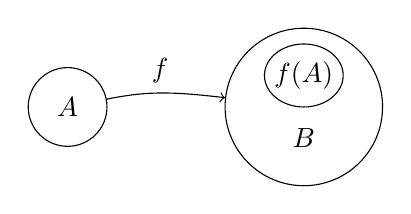
\begin{tikzpicture}
            \node (A) at (-1,0) [draw, circle, minimum size=1cm] {$A$};

            \node (B) at (2,0) [draw, circle, minimum size=2cm] {};
            \draw (2,0.4) ellipse [x radius=0.5, y radius=0.4] node {$f(A)$};
            \node at (2,-0.4) {$B$};

            \draw[->] (A) .. controls (0,0.2) and (0.3,0.2) .. (B) node[midway, above] {$f$};
        \end{tikzpicture}
        \hspace*{2cm}
        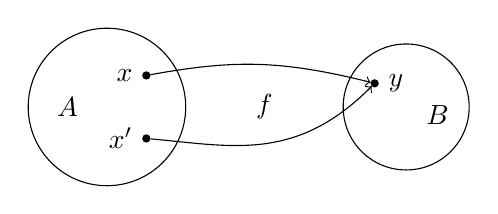
\begin{tikzpicture}[p/.style={fill, circle, minimum size=3pt, inner sep=0pt, outer sep=0pt}]
            %There is no way to name `pic` coordinates. It seems to be a bug, see https://tex.stackexchange.com/questions/194362.
            \draw (-1,0) circle [radius=1];
            \node[label=left:$x$, p] (x) at (-0.5,0.4) {};
            \node[label=left:$x'$, p] (x') at (-0.5,-0.4) {};
            \node at (-1.5,0) {$A$};

            \draw (2.8,0) circle [radius=0.8];
            \node[label=right:$y$, p] (y) at (2.4,0.3) {};
            \node at (3.2,-0.1) {$B$};

            \draw[->] (x) .. controls (0.6,0.6) and (1.2,0.6) .. (y);
            \draw[->] (x') .. controls (0.6,-0.5) and (1.4,-0.7) .. (y);
            \node at (1,0) {$f$};
        \end{tikzpicture}
        \caption{Links: $f$~ist \emph{nicht surjektiv}. Rechts: $f$~ist \emph{nicht injektiv}.}
    \end{figure}
\end{definition}

Die folgenden Definitionen gehen auf \textsc{Georg Cantor} zurück.

\begin{definition}[Gleichmächtigkeit, Abzählbarkeit]\leavevmode
    \begin{enumerate}
        \item Mengen $A$~und~$B$ heißen \emph{gleichmächtig}, falls es eine bijektive Abbildung $f\colon A \to B$ gibt.
        \item Eine Menge~$A$ heißt \emph{abzählbar unendlich}, falls sie zu~$\N$ gleichmächtig ist.
        \item Eine Menge~$A$ heißt \emph{abzählbar}, falls sie leer, endlich oder abzählbar unendlich ist. Andernfalls heißt $A$ \emph{überabzählbar}.
    \end{enumerate}
\end{definition}

Die Idee der Gleichmächtigkeit ist, dass eine Reihenfolge gefunden werden kann, in der alle Elemente der Menge vorkommen, sprich wir können die Elemente der Menge~$M$ durchnummerieren mit~$M = \mset{a_1, a_2, a_3, \dots}$. Damit erhalten wir eine Bijektion zwischen den Indizes (den natürlichen Zahlen) und den Elementen.

\lecturesep{03.~November 2021}

\begin{example}\leavevmode
    \begin{enumerate}
        \item $\N$,~$\Z$ und~$\Q$ sind abzählbar.

              $\N$~ist offensichtlich abzählbar. Für~$\Z$ können wir die Reihenfolge $\Z = \mset{0, 1, -1, 2, -2, 3, -3, \dots}$ definieren, sodass wir jedem Element seine Stelle in der Auflistung (eine natürliche Zahl) zuordnen:
              \begin{gather*}
                  \begin{matrix}
                      0            & 1            & -1           & 2            & -2           & 3            & -3           & \dots \\
                      \updownarrow & \updownarrow & \updownarrow & \updownarrow & \updownarrow & \updownarrow & \updownarrow &       \\
                      1            & 2            & 3            & 4            & 5            & 6            & 7            & \dots
                  \end{matrix}
                  \qquad\text{bzw.}\qquad
                  f(n) = \begin{cases}
                      \frac{1}{2}n,     & \text{falls $n$~gerade},   \\
                      \frac{1}{2}(1-n), & \text{falls $n$~ungerade}.
                  \end{cases}
              \end{gather*}

              Für~$\Q$ erfolgt ein Beweis weiter unten.
        \item $\R$~ist überabzählbar. Auch das beweisen wir unten.
    \end{enumerate}
\end{example}

\begin{theorem}
    $\Q$~ist abzählbar.
\end{theorem}

\begin{proof}
    Jeden Bruch~$q \in \Q$ können wir als Quotienten~$q = m/n$ mit teilerfremden~$m \in \Z$ und~$n \in \N$ schreiben. Wir betrachten alle~$(m, n)$ als Punkte im Gitter~$\Z^2 \subset \R^2$:
    \begin{center}
        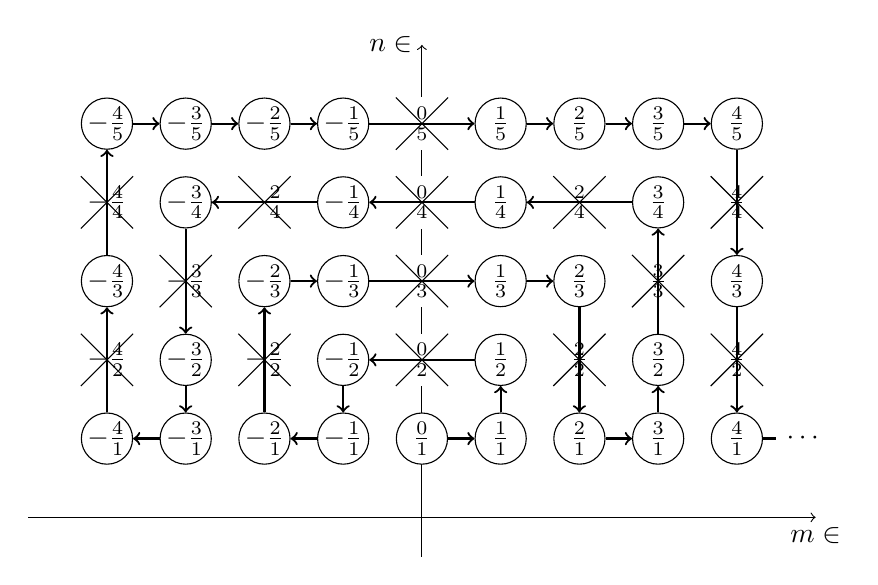
\begin{tikzpicture}[
                circ/.style={circle, draw, fill=white, minimum size=0.65cm, inner sep=0pt},
                rect/.style={rectangle, draw=white, fill=white, minimum size=0.65cm, inner sep=0pt},
                cross/.style={rect, append after command={(\tikzlastnode.north west) edge (\tikzlastnode.south east) (\tikzlastnode.north east) edge (\tikzlastnode.south west)}}]
            \draw[->] (-5,0) -- (5,0) node[below] {$m \in \Z$};
            \draw[->] (0,-0.5) -- (0,6) node[left] {$n \in \N$};

            \foreach \m in {-4,...,4} {
                    \foreach \n in {1,...,5} {
                            \tikzmath{
                                if gcd(\m,\n) == 1 then {
                                        let \style = circ;
                                    } else {
                                        let \style = cross;
                                    };
                                int \sabs;
                                if sign(\m) == -1 then {
                                        let \ssign = -;
                                        \sabs = abs(\m);
                                    } else {
                                        let \ssign = ;
                                        \sabs = \m;
                                    };
                            }
                            \node[draw, \style] (\m\n) at (\m,\n) {$\ssign\frac{\sabs}{\n}$};
                        }
                }

            \foreach \a [remember=\a as \b (initially 01)] in {11, 12, -12, -11, -21, -23, -13, 13, 23, 21, 31, 32, 34, 14, -14, -34, -32, -31, -41, -43, -45, -35, -25, -15, 15, 25, 35, 45, 43, 41}
            \draw[->, thick] (\b) -- (\a);
            \draw[thick] (41) -- (4.5,1) node[right] {$\cdots$};
        \end{tikzpicture}
    \end{center}

    Die teilerfremden~$(m, n)$ werden behalten, während die nicht teilerfremden~$(m, n)$ rausgestrichen werden. Wir durchlaufen alle Gitterpunkte in "`konzentrischen Kreisen"' um~0 und betrachten dabei nur die teilerfremden Paare~$(m, n)$. Damit können wir alle~$q$ durchnummerieren.\footnote{Das ist eine alternative Version des \emph{ersten \textsc{cantorschen} Diagonalargument}. Für die originale Idee nehmen wir nur den ersten Quadraten der Abbildung, also~$\Q^+$. Nun zeichnen wir Diagonalen mit Anstieg~$-1$ und verbinden sie so parallel zu den Achsen, dass eine "`Schlangenlinie"' über die Diagonalen entsteht. Streichen wir noch die nicht teilerfremden Paare~$(m, n)$, haben wir eine Reihenfolge und $\Q^+$~und~$\N$ sind gleichmächtig. Fügen wir vor der Schlangenlinie die Null, und hinter jedem~$(m, n)$ noch~$(-m, n)$ hinzu, sind auch $\Q$~und~$\N$ gleichmächtig. Mehr dazu s.~\url{https://de.wikipedia.org/wiki/Cantors_erstes_Diagonalargument}.}
\end{proof}

\begin{remark}\leavevmode
    \begin{enumerate}
        \item Mit analogen Verfahren können wir auch $\N \times \N$ oder $\Z \times \Z$ durchnummerieren.
              \begin{center}
                  \begin{tikzpicture}[scale=0.4, baseline=(current bounding box.center)]
                      \draw[->] (0,0) -- (0,6);
                      \draw[->] (0,0) -- (6,0);
                      \foreach \x in {1,...,5} \foreach \y in {1,...,5} \pic at (\x,\y) {dot};
                  \end{tikzpicture}
                  \hspace*{1cm}
                  \begin{tikzpicture}[scale=0.4, baseline=(current bounding box.center)]]
                    \draw[->] (0,-3) -- (0,3);
                    \draw[->] (-3,0) -- (3,0);
                    \foreach \x in {-2,...,2} \foreach \y in {-2,...,2} \pic at (\x,\y) {dot};
                  \end{tikzpicture}
              \end{center}
        \item Die naive Idee, zuerst alle~$q$ mit~$n = 1$, dann~$n = 2$ etc.\ durchzugehen funktioniert \emph{nicht}, da es unendlich viele~$q$ in der Reihe~$n = 1$ gibt und wir nie zu~$n > 1$ kommen.
    \end{enumerate}
\end{remark}

\begin{theorem}
    $\R$~ist nicht abzählbar.
\end{theorem}

\begin{proof}[Beweis durch Intervallschachtelung]
    Wir nehmen an, dass~$\R = \mset{x_1, x_2, \dots}$ abzählbar ist. Nun definieren wir eine Intervallschachtelungen~$(I_n)_n$ rekursiv: $I_1 = [x_1+1, x_1+2]$; zerlege~$I_n$ in drei gleichlange Teilintervalle und wähle eines dieser als~$I_{n+1}$ so aus, dass $x_{n+1}$ nicht in~$I_{n+1}$ enthalten ist. Nach Intervallschachtelungsprinzip gibt es ein~$s \in \R$ mit~$s \in \bigcap_n I_n$. Das bedeutet aber auch, dass es ein~$k \in \N$ geben muss mit $s = x_k \in \R$. Nach Konstruktion der~$I_k$ ist~$x_k \notin I_k$, aber~$s \in I_k$, ein Widerspruch.
\end{proof}

Im Beweis reicht es nicht, $I_n$~zu halbieren, da~$x_{n+1}$ die Mitte von~$I_n$ sein kann und damit in beiden Teilintervallen liegt.

\begin{proof}[Alternativer Beweis]
    Wir verwenden die dyadische (binäre) Darstellung der reellen Zahlen. Angenommen $[0, 1) = \mset{x_1, x_2, \dots}$ ist abzählbar, d.\,h.\ wir können eine Liste aller Zahlen
    \begin{align*}
        x_1 & = 0,\underline{a_{11}}a_{12}a_{13}\dots \\
        x_1 & = 0,a_{11}\underline{a_{12}}a_{13}\dots \\
        x_1 & = 0,a_{11}a_{12}\underline{a_{13}}\dots \\
        \vdotswithin{=}
    \end{align*}
    mit~$a_{ij} \in \mset{0, 1}$ für alle~$i, j \in \N$.

    Nun konstruieren wir eine neue Zahl~$y = 0,b_{11}b_{12}b_{13}\dots$ mit~$b_i = 1-a_{ii}$ für alle~$i$. Nun unterscheiden sich $y$ und jedes~$x_i$ an der $i$"~ten Stelle, weshalb $y$~nicht in der Liste liegt, also~$y \notin \mset{x_i : i \in \N} = [0, 1)$, Widerspruch.\footnote{Der Beweis (aber im Dezimalsystem) ist bekannt als das \emph{zweite \textsc{cantorsche} Diagonalargument}.}
\end{proof}

\begin{remark}
    Streng genommen müssen wir für den Beweis noch zeigen, dass jede reelle Zahl in~$[0, 1)$ sich im Binärsystem darstellen lässt, also~$z = \sum_{i=0}^\infty z_i 2^{-i}$ in~$\R$ konvergiert und jede binäre Repräsentation einer reellen Zahl auch eindeutig ist.
\end{remark}

\begin{corollary}
    $\R \setminus \Q$ ist nicht abzählbar.
\end{corollary}

\begin{remark}
    Folgende Aussagen werden noch in den Übungen gezeigt.
    \begin{enumerate}
        \item Die Menge \emph{aller Teilmengen} aus~$\N$ ist überabzählbar. Die Menge aller \emph{endlichen} Teilmengen aus~$\N$ ist abzählbar.
        \item Die Menge \emph{aller Folgen} mit Werten in~$\mset{0, 1}$ ist überabzählbar. Die Menge aller \emph{endlichen} Folgen mit Werten in~$\Q$ ist abzählbar.
    \end{enumerate}
\end{remark}

\subsubsection{Kontinuumshypothese}

(\textsc{Cantor} 1878). \emph{Es existiert keine Menge, deren Mächtigkeit zwischen der von~$\N$ und von~$\R$ liegt.}

Diese Aussage ist mit den üblichen Axiomen der Mengenlehre (\emph{\textsc{Zermelo}-\textsc{Frankel}-Mengenlehre}) weder beweisbar noch widerlegbar (Nichtwiderlegbarkeit durch \textsc{Kurt Gödel} 1940, Nichtbeweisbarkeit durch \textsc{Paul Cohen} 1963).\footnote{Unser Dozent rechnete fälschlicherweise die Unentscheidbarkeit der Kontinuumshypothese \textsc{Gödel} im Jahr~1938 zu.}

\section{Konvergenz von Folgen~II}

\subsection{Monotone Folgen}

\begin{definition}[schwach waschend/fallend, monoton]
    Eine Folge~$(a_n)_{n\in\N}$ von reellen Zahlen heißt
    \begin{itemize}
        \item \emph{schwach wachsend} (nicht fallend), falls $a_n \leq a_{n+1}$ für alle~$n \in \N$ gilt,
        \item \emph{schwach fallend} (nicht wachsend), falls $a_n \geq a_{n+1}$ für alle~$n \in \N$ gilt, und
        \item \emph{monoton}, falls sie schwach wachsend oder schwach fallend ist.
    \end{itemize}
\end{definition}

\begin{theorem}[Konvergenz beschränkter monotoner Folgen]\label{thm:bound2}
    Jede beschränkte monotone Folge~$(a_n)_{n\in\N}$ reeller Zahlen konvergiert, und zwar
    \begin{itemize}
        \item gegen~$\sup A = \mset{a_n}$, falls $(a_n)$~schwach wachsend ist, und
        \item gegen~$\inf A = \mset{a_n}$, falls $(a_n)$~schwach fallend ist.
    \end{itemize}
\end{theorem}

\begin{proof}
    Wir beweisen den Satz für schwach wachsende Folgen. Für schwach fallende Folgen erfolgt der Beweis analog.

    Sei~$a = \sup A$. Dann gibt es für jedes~$\eps > 0$ ein~$N \in \N$, sodass $a - \eps \leq a_N$ gilt (ansonsten wäre $a - \eps$ eine obere Schranke der Folge). Mit der Monotonie gilt nun für alle~$n \geq N$: $a - \eps \leq a_n \leq a$, also $a_n \to a$ für~$n \to \infty$.
\end{proof}

Vgl.~den Satz mit \cref{thm:bound}, der besagt, dass jede konvergente Folge beschränkt ist.

\subsection{Uneigentliche Konvergenz}

Unser Ziel ist es, sagen zu können, dass \emph{jede} (auch unbeschränkte) monotone Folge "`konvergiert"'. Unsere bisherige \cref{def:convergence} im (strikten) Sinne erlaubt nur Konvergenz gegen reelle Zahlen. Wir erweitern also den Begriff, sodass unbeschränkte monotone Folgen auch gegen~$+\infty$ oder~$-\infty$ konvergieren können.

\begin{definition}[erweiterte Zahlengerade]
    Sei die \emph{erweiterte Zahlengerade} (auch die \emph{erweiterten reellen Zahlen}) $\exR \coloneqq \R \cup \mset{-\infty, +\infty}$ die um zwei Elemente~$\pm\infty$ ("`plus/minus unendlich"') erweiterte Menge der reellen Zahlen~$\R$.

    Für~$\pm\infty$ werden folgende Rechenregeln für alle~$x \in \R$ definiert:
    \begin{itemize}
        \item $-\infty < x < +\infty$;
        \item $(\pm\infty) + x = \pm\infty$, genauso gelten hierfür Kommutativität, Assoziativität und Distributivität;
        \item für~$x > 0$: $(\pm\infty) x = \pm\infty$, hierfür gelten auch Kommutativität, Assoziativität, Distributivität;
        \item für~$x < 0$: $(\pm\infty) x = \mp\infty$;
        \item $(-\infty) + (+\infty)$ ist nicht definiert;
        \item $(\pm\infty) \cdot 0$ ist nicht definiert.\footnote{Weitere nicht definierte Ausdrücke sind $x/0$, $(\pm\infty) / (\pm\infty)$ und $(\pm\infty) / (\mp\infty)$. Hingegen gilt zusätzlich für die Division $x / (\pm\infty) = 0$, $(\pm\infty) / x = \pm\infty$ für~$x > 0$ und $(\pm\infty) / x = \mp\infty$ für~$x < 0$.}
    \end{itemize}

    Ferner sind $\exR = [-\infty, +\infty]$, $\R = (-\infty, +\infty)$ und für alle~$a, b \in \exR$ mit~$a < b$ die Intervalle $[a, b]$, $[a, b)$, $(a, b]$ und~$(a, b)$ wie gewohnt (d.\,h.\ analog zu \cref{def:interval}) definiert.
\end{definition}

\begin{definition}[uneigentliche Konvergenz]
    Eine Folge~$(a_n)_{n\in\N}$ reeller Zahlen \emph{konvergiert uneigentlich gegen $+\infty$} (geschrieben $a_n \to +\infty$), falls für jedes~$k \in \R$ ein~$N \in \N$ existiert, sodass $a_n \geq k$ für alle~$n \geq N$ gilt. Analog ist die \emph{uneigentliche Konvergenz gegen $-\infty$} definiert ($a_n \to -\infty$).
\end{definition}

\emph{Achtung}: Die Folge~$(a_n)_n$ \emph{konvergiert}, falls sie gegen ein~$a \in \R$ konvergiert. Sie ist hingegen \emph{uneigentlich konvergent}, falls sie gegen $+\infty$~oder~$-\infty$ konvergiert. Wenn wir also nicht spezifizieren, ist Konvergenz in~$\R$ gemeint, und Divergenz kann uneigentliche Konvergenz oder Divergenz in~$\exR$ bedeuten.

\begin{remark}
    Durch die bijektive Abbildung~$\sigma\colon \exR \to [-1, 1]$, $x \mapsto x / (1+\abs{x})$ mit $\sigma(+\infty) \coloneqq 1$ und $\sigma(-\infty) \coloneqq -1$ werden die Ordnungsstrukturen von~$\bar{R}$ und~$[-1, 1]$ ineinander überführt.\footnote{$\sigma$~ist ein sog.\ \emph{Homöomorphismus}, da die Abbildung bijektiv und stetig sowie die Umkehrabbildung auch stetig ist. Damit werden die Strukturen zwischen beiden Räumen erhalten (sind also \emph{homöomorph}).} Ferner gilt deshalb: Eine Folge~$(x_n)_{n\in\N}$ konvergiert (uneigentlich) gegen ein~$x \in \bar{R}$ genau dann, wenn die Folge~$(\sigma(x_n))_{n\in\N}$ gegen ein~$\sigma(x) \in [-1, 1]$ konvergiert.
    \begin{center}
        \begin{tikzpicture}
            \draw[->] (0,-1.3) -- (0,1.3);
            \draw[->] (-3,0) -- (3,0) node[below] {$\exR$};
            \pic at (0,1) {ytick=1};
            \pic at (0,-1) {ytick=$-1$};
            \draw[domain=-6:6, smooth] plot ({0.5*\x},{\x / (1 + abs(\x))}) node[right] {$\sigma(x) = \dfrac{x}{1 + \abs{x}}$};
        \end{tikzpicture}
    \end{center}
\end{remark}

\emph{Achtung}: Beim Rechnen mit~$\pm\infty$ gelten nicht alle Regeln aus~$\R$ wie gewohnt (ansonsten kommen Widersprüche auf). Dasselbe gilt auch für das Rechnen mit uneigentlich konvergenten Folgen.

\subsection{Limes Superior und Limes Inferior}

\begin{definition}[Limes Superior/Inferior]
    Sei~$(a_n)_{n\in\N}$ eine Folge reeller Zahlen und seien $b_n = \sup\mset{a_k : k \geq n}$ und $c_n = \inf\mset{a_k : k \leq n}$. Dann sind $(b_n)_{n\in\N}$ eine schwach fallende und $(c_n)_{n\in\N}$ eine schwach wachsende Folge\footnote{Eine kurze Begründung dafür: Nach Definition ist $b_n \geq a_k$ für alle~$k \geq n$, also auch $b_n \geq a_k$ für alle~$k \geq n+1$, d.\,h.\ $b_n$~ist eine obere Schranke von $\mset{a_k : k \geq n+1}$. Aufgrund der Minimalität des Supremums muss dann $b_n \geq b_{n+1} = \sup\mset{a_k : k \geq n+1}$ sein. Analog lässt sich für~$c_n$ argumentieren.} in~$\exR$, die auch (uneigentlich in~$\exR$) konvergieren. Dann sind
    \begin{equation*}
        \limsup_{n\to\infty} a_n \coloneqq \varlimsup_{n\to\infty} a_n \coloneqq \lim_{n\to\infty} b_n \qquad\text{und}\qquad \liminf_{n\to\infty} a_n \coloneqq \varliminf_{n\to\infty} a_n \coloneqq \lim_{n\to\infty} c_n
    \end{equation*}
    der \emph{Limes Superior} bzw.\ der \emph{Limes Inferior}.\footnote{Die Idee des Limes Superior bzw.\ Inferior ist es, eine neue Weise einzuführen, um Folgen zu beschreiben. Bisher kennen wir nur die Konvergenz gegen eine Zahl, aber was ist, wenn die Folge divergiert? Dann kann es trotzdem sein, dass sie beschränkt ist (wie z.\,B.\ $\paren*{(-1)^n}_n$, aber in~$\exR$ eigentlich immer), und wir können versuchen Aussagen über die Grenzwerte der Schranken zu machen. Mit dem Limes Superior bzw.\ Inferior können wir also den "`Grenzwert"' zu einem "`Grenzbereich"' erweitern, worin ab einem bestimmten Folgenglied alle Folgenglieder im Intervall $[\liminf a_n-\eps,\; \limsup a_n+\eps]$ für beliebig kleine~$\eps$ liegen.}
\end{definition}

Wegen der Monotonie von $(b_n)$~bzw.~$(c_n)$ gilt
\begin{equation*}
    \limsup_{n\to\infty} a_n = \inf_n b_n \qquad\text{und}\qquad \liminf_{n\to\infty} a_n = \sup_n c_n,
\end{equation*}
oder mit anderen Worten
\begin{lemma}\label{lem:infsup}
    Es gelten
    \begin{equation*}
        \limsup_{n\to\infty} a_n = \adjustlimits\lim_{n\to\infty} \sup_{k\geq n} a_k = \adjustlimits\inf_{n\in\N} \sup_{k\geq n} a_k \qquad\text{und}\qquad \liminf_{n\to\infty} a_n = \adjustlimits\lim_{n\to\infty} \inf_{k\geq n} a_k = \adjustlimits\sup_{n\in\N} \inf_{k\geq n} a_k.
    \end{equation*}
\end{lemma}

\begin{example}\leavevmode
    \begin{enumerate}
        \item Für $(a_n)_{n\in\N}$ mit~$a_n = n$ sind $b_n = \sup\mset{a_k : k \geq n} = +\infty$ und $c_n = \inf\mset{a_k : k \geq n} = n$ für alle~$n$. Damit sind $\limsup_{n\to\infty} a_n = \lim_{n\to\infty} b_n = +\infty$ und $\liminf_{n\to\infty} a_n = \lim_{n\to\infty} c_n = +\infty$.
        \item Für $a_n = (-1)^n (1-1/n)$, also $\paren*{0, +\frac{1}{2}, -\frac{2}{3}, +\frac{3}{4}, -\frac{4}{5}, \dots}$, sind $b_n = \sup\mset{a_k : k \geq n} = +1$ und $c_n = \inf\mset{a_k : k \geq n} = -1$. Damit sind $\limsup_{n\to\infty} a_n = +1$ und $\liminf_{n\to\infty} a_n = -1$.
        \item Für $a_n = (-1)^n (1+1/n)$ sind
              \begin{equation*}
                  b_n = \begin{cases}
                      1 + \frac{1}{n}   & \text{für gerade }n,   \\
                      1 + \frac{1}{n+1} & \text{für ungerade }n,
                  \end{cases}\qquad\text{und}\qquad
                  c_n = \begin{cases}
                      1 + \frac{1}{n}   & \text{für ungerade }n, \\
                      1 + \frac{1}{n+1} & \text{für gerade }n.
                  \end{cases}
              \end{equation*}
              Daraus folgen $\limsup_{n\to\infty} a_n = \lim_{n\to\infty} b_n = +1$ und $\liminf_{n\to\infty} = \lim_{n\to\infty} c_n = -1$.

              \begin{figure}
                  \begin{tikzpicture}[baseline=(current bounding box.base)]
                      \draw[->] (0,-1.3) -- (0,1.3);
                      \draw[->] (-0.3,0) -- (3.3,0);
                      \pic at (0,1) {ytick=1};
                      \pic at (0,-1) {ytick=$-1$};
                      \draw[domain=1:12, smooth] plot ({0.25*\x},{1-1/\x});
                      \draw[domain=1:12, smooth] plot ({0.25*\x},{-(1-1/\x)});
                  \end{tikzpicture}
                  \hspace*{1cm}
                  \begin{tikzpicture}[baseline=(current bounding box.base)]
                      \draw[->] (0,-1.3) -- (0,1.3);
                      \draw[->] (-0.3,0) -- (3.3,0);
                      \pic at (0,0.5) {ytick=1};
                      \pic at (0,-0.5) {ytick=$-1$};
                      \draw[domain=1:12, smooth] plot ({0.25*\x},{(0.5*(1+1/\x)});
                      \draw[domain=1:12, smooth] plot ({0.25*\x},{-0.5*(1+1/\x)});
                  \end{tikzpicture}
                  \caption{Veranschaulichung der Beispiele. Links: $a_n = (-1)^n(1-1/n)$. Rechts: $a_n = (-1)^n (1+1/n)$.}
              \end{figure}
    \end{enumerate}
\end{example}

\begin{remark}
    Es gilt stets $\liminf_{n\to\infty} a_n \leq \limsup_{n\to\infty} a_n$, was aus $\inf_{n\geq k} a_k \leq \sup_{n\geq k} a_k$ und der Ordnungserhaltung von konvergierenden Folgen folgt (\cref{thm:sequence:monotony}).
\end{remark}

\lecturesep{08.~November 2021}

\begin{theorem}\label{thm:convergence:exr}
    Jede monotone Folge in~$\R$ konvergiert in~$\exR$.
\end{theorem}

\begin{proof}
    O.\,B.\,d.\,A.\ sei $(a_n)_n$ schwach wachsend. Dann unterscheiden wir zwei Fälle:
    \begin{enumerate}
        \item Wenn $\sup_n a_n$ endlich ist, dann ist $(a_n)_n$ nach oben beschränkt, und aufgrund \cref{thm:bound2} konvergiert die Folge gegen~$\sup_n a_n$.
        \item Wenn~$\sup_n a_n = +\infty$, dann gibt es für jedes~$k \in \R$ ein~$N \in \N$ mit~$a_N \geq k$ (andernfalls ist~$\sup_n a_n$ nicht die kleinste obere Schranke mehr). Aufgrund Monotonie gilt~$a_n \geq k$ für alle~$n \geq N$. Das ist die Definition der uneigentlichen Konvergenz, also $a_n \to +\infty$ für~$n \to \infty$.\qedhere
    \end{enumerate}
\end{proof}

\begin{theorem}
    Eine reelle Zahlenfolge~$(a_n)_{n\in\N}$ konvergiert (bzw.\ konvergiert in~$\exR$) genau dann, wenn $\limsup a_n = \liminf a_n \in \R$ (bzw.\ $\limsup a_n = \liminf a_n \in \exR$). In diesem Fall ist $\lim a_n = \liminf a_n = \limsup a_n$.
\end{theorem}

\begin{proof}
    Wir zeigen die Behauptung für Konvergenz in~$\R$. Für die uneigentliche Konvergenz kann man ähnlich verfahren.

    Zur Hinrichtung: Angenommen $(a_n)_n$~konvergiert gegen~$a \in \R$. Dann gibt es für jedes~$\eps > 0$ ein~$N \in \N$, sodass $\abs{a_n-a} < \eps \iff a-\eps < a_n < a+\eps$ für alle~$n \geq N$ gilt.

    Aus~$a_n < a+\eps$ folgt $b_N \coloneqq \sup_{n\geq N} a_n \leq a+\eps$. Da $(b_n)$ eine schwach fallende folgende Folge ist, gilt für alle~$n \geq N$ dann $b_n \leq b_N \leq a+\eps$, also $\lim_{n\to\infty} b_n \leq a+\eps$.

    Analog verfahren wir mit~$a_n > a-\eps$, sodass wir $c_N \coloneqq \inf_{n\geq N} a_n \geq a-\eps$, also $\lim_{n\to\infty} c_n \geq a-\eps$ erhalten. Mit $\liminf a_n \leq \limsup a_n$ erhalten wir
    \begin{equation*}
        a-\eps \leq \lim_{n\to\infty} c_n = \liminf_{n\to\infty} a_n \leq \limsup_{n\to\infty} a_n = \lim_{n\to\infty} b_n \leq a+\eps,
    \end{equation*}
    wobei für beliebig kleine~$\eps > 0$ Gleichheit gilt.

    Zur Rückrichtung: Angenommen es gilt $\liminf a_n = a = \limsup a_n \in \R$. Dann gibt aufgrund des Konvergenzkriteriums für jedes~$\eps > 0$ ein~$N \in \N$, sodass $b_N \leq a+\eps$ und $c_N \geq a-\eps$ gilt. Wegen der Definition der Suprema/Infima haben wir $a_n \leq a+\eps$ und $a_n \geq a-\eps$ für alle~$n \geq N$, also $\abs{a_n-a} < \eps$ und daher~$a_n \to a$.
\end{proof}

\subsection{Teilfolgen und Häufungspunkte}

\begin{definition}[Teilfolge, Häufungspunkt]\leavevmode
    \begin{enumerate}
        \item Sei~$(a_n)_{n\in\N}$ eine reelle Zahlenfolge und $(n_k)_{k\in\N}$ eine strikt wachsende Folge in~$\N$. Dann heißt die Folge~$(a_{n_k})_{k\in\N} = (a_{n_1}, a_{n_2}, a_{n_3}, \dots)$ \emph{Teilfolge} der Folge~$(a_n)_{n\in\N}$.
        \item $a \in \R$~heißt \emph{Häufungspunkt} der Folge~$(a_n)_{n\in\N}$, wenn es eine Teilfolge von~$(a_n)_n$ gibt, die gegen~$a$ konvergiert.
    \end{enumerate}
\end{definition}

\begin{example}\leavevmode
    \begin{enumerate}
        \item $a_n = (-1)^n$, dann sind 1~und~$-1$ Häufungspunkte, denn $1 = \lim_{k\to\infty} a_{2k}$ und $-1 = \lim_{k\to\infty} a_{2k+1}$ (also $n_k = 2k$ bzw.\ $n_k = 2k+1$).
        \item Teilfolgen der Folge~$(1/n)_{n\in\N}$ sind z.\,B.\ $\paren*{2^{-k}}_{k\in\N}$, $(1/k!)_{k\in\N}$, $(1/p)_{p\text{ prim}}$, etc.
    \end{enumerate}
\end{example}

\begin{remark}\label{rem:subsequence:convergence}
    Jede Teilfolge einer \emph{konvergenten Folge} konvergiert und besitzt denselben Grenzwert (das folgt sofort aus der Konvergenzdefinition). D.\,h.\ jede konvergente Folge besitzt genau einen Häufungspunkt, nämlich den Grenzwert selbst.\footnote{Die Umkehrung gilt auch: Konvergiert jede Teilfolge, so konvergiert auch die Folge selbst, denn die Folge selbst ist ja auch eine Teilfolge von sich selbst.}
\end{remark}

\begin{lemma}
    $a \in \R$~ist genau dann ein Häufungspunkt von~$(a_n)_{n\in\N}$, wenn es für jedes~$\eps > 0$ unendlich viele~$n \in \N$ gibt mit $\abs{a_n-a} < \eps$.
\end{lemma}

\begin{proof}
    Zur Hinrichtung: Ist $a$~ein Häufungspunkt von~$(a_n)$, so gibt es eine Folge~$(n_k)_k$ natürlicher Zahlen und ein~$K \in \N$, sodass $\abs{a_{n_k}-a} \leq \eps$. Also gibt es unendlich viele~$n \in \N$, die das erfüllen, nämlich $n \in \mset{n_K, n_{K+1}, n_{K+2}, \dots}$.

    Zur Rückrichtung: Wir werden eine streng wachsende Folge~$(n_k)_k$ in~$\N$ rekursiv konstruieren, sodass die Teilfolge~$(a_{n_k})_k$ gegen~$a$ konvergiert. Dazu wählen wir~$\eps = 1/k$ im Konvergenzkriterium. Sei~$n_1$ so gewählt mit $\abs{a_{n_1}-a} < 1/1$. Für folgende~$k > 1$ wählen wir~$n_k$ so von den unendlich vielen~$n$, dass $\abs{a_{n_k}-a} < 1/k$ und $n_k$~größer als alle vorher gewählten $n_1, n_2, \dots, n_{k-1}$ ist. Damit gilt $a_{n_k} \to a$.
\end{proof}

Nun zu einem wichtigen Satz der Analysis:

\begin{theorem}[\textsc{Bolzano}-\textsc{Weierstraß}]
    Für jede beschränkte reelle Zahlenfolge~$(a_n)_{n\in\N}$ gilt:
    \begin{enumerate}
        \item $\liminf_{n\to\infty} a_n$ und $\limsup_{n\to\infty} a_n$ sind Häufungspunkte.
        \item Für jeden Häufungspunkt~$a \in \R$ gilt
              \begin{equation*}
                  \liminf_{n\to\infty} a_n \leq a \leq \limsup_{n\to\infty} a_n.
              \end{equation*}
    \end{enumerate}
    Mit anderen Worten: $\liminf_{n\to\infty} a_n$ und $\limsup_{n\to\infty} a_n$ sind der kleinste bzw.\ größte Häufungspunkt.
\end{theorem}

\begin{proof}\leavevmode
    \begin{enumerate}
        \item Wir konstruieren rekursiv~$(n_k)_{k\in\N}$ in~$\N$ mit $a_{n_k} \to \limsup_{n\to\infty}$ für~$k \to \infty$. Die Konstruktion für $a_{n_k} \to \liminf_{n\to\infty}$ ist ähnlich.

              Für den Rekursionsanfang setzen wir~$n_1 = 1$. Für den Rekursionsschritt sei~$n_k$ gegeben. Wir betrachten
              \begin{equation*}
                  b_{1+n_k} \coloneqq \sup\mset{a_{1+n_k}, a_{2+n_k}, a_{3+n_k}, \dots}.
              \end{equation*}
              Diese Zahl ist reell, weil $(a_n)_n$ beschränkt ist. Da sie auch die kleinste obere Schranke der obigen Menge ist, gibt es ein~$n_{k+1} \in \mset{1+n_k, 2+n_k, 3+n_k, \dots}$ mit $a_{n_{k+1}} \geq b_{1+n_k} - 1/k$ (andernfalls wäre auch $b_{1+n_k} - 1/k$ eine obere Schranke). Daher gilt für alle~$k \in \N$:
              \begin{equation*}
                  b_{1+n_k} \geq a_{n_{k+1}} \geq b_{1+n_k} - \frac{1}{k}.
              \end{equation*}
              Nun wissen wir, dass $(b_{1+k_n})_k$ monoton schwach fällt und deshalb konvergiert (\cref{thm:bound2}). Aus der eben gezeigten Ungleichung folgt also für beliebig kleine~$1/k$, dass $(a_{n_k})_{k\in\N}$ konvergiert, nämlich gegen den Grenzwert von~$(b_{1+n_k})_k$. Da $(b_{1+n_k})_k$~eine Teilfolge von~$(b_n)_n$ (es sei $b_n \coloneqq \sup_{k\geq n} a_k$) ist, konvergieren $(a_{n_k})_k$ und $(b_{n_k})_k$ gegen den Grenzwert von~$(b_n)_n$, also $a_{n_k} \to \limsup_n a_n$.

        \item Sei~$a = \lim_{k\to\infty} a_{n_k}$. Dann gibt es für jedes~$\eps > 0$ ein~$K \in \N$, sodass $\abs{a-a_{n_k}} < \eps$ für alle~$k \geq K$ gilt. Daraus folgt $a \leq a_{n_k} + \eps \leq \sup\mset{a_n : n \geq n_k} + \eps$ . Für~$k \to \infty$ ergibt sich $a \leq \limsup_{n\to\infty} a_n + \eps$, und für beliebig kleine~$\eps > 0$ schließlich $a \leq \limsup_{n\to\infty} a_n$. Analog würden wir $a \geq \liminf_{n\to\infty} a_n$ erhalten.\qedhere
    \end{enumerate}
\end{proof}

\begin{corollary}
    Jede beschränkte Zahlenfolge besitzt (mindestens) eine konvergente Teilfolge.\footnote{In den meisten Lehrbüchern wird das als Satz von Bolzano-Weierstraß bezeichnet.}
\end{corollary}

\begin{corollary}
    Jede reelle Zahlenfolge besitzt (mindestens) eine in~$\exR$ konvergente Teilfolge.
\end{corollary}

\section{Konvergenz von Reihen}

\subsection{Unendliche Reihen}

\begin{definition}[Partialsumme, Reihe]
    Gegeben sei eine reelle Zahlenfolge~$(a_n)_{n\in\N}$ (nicht in~$\exR$!). Dann ist $(s_n)_{n\in\N}$ die \emph{Folge der Partialsummen} $s_n = \sum_{k=1}^n a_k$ (zum Teil auch~$(a_n)_{n\in\N_0}$ und $s_n = \sum_{k=0}^n a_k$).

    Als \emph{unendliche Reihe}~$\sum_k a_k$ bezeichnen wir
    \begin{itemize}
        \item einerseits die Folge~$(s_n)_{n\in\N}$ und
        \item andererseits deren Grenzwert $\lim_{n\to\infty} s_n = \lim_{n\to\infty} \sum_{k=1}^n a_k = \sum_{k=1}^\infty a_k$.
    \end{itemize}
\end{definition}

\begin{example}\leavevmode
    \begin{enumerate}
        \item Die \emph{geometrische Reihe} $\sum_{k=0}^\infty q^k = 1/(1-q)$ für alle~$q \in \R$ mit~$\abs{q} < 1$.
        \item Die \emph{harmonische Reihe} $\sum_{n=1}^\infty 1/n = +\infty$. Die geometrische und harmonische Reihe sind sehr wichtig ("`Mütter aller Reihen"').
        \begin{proof}[Beweis (unformal)]
            Es gilt
            \begin{equation*}
                1 + \underbrace{\frac{1}{2}}_{\geq 1/2} + \underbrace{\frac{1}{3} + \frac{1}{4}}_{\geq 1/2} + \underbrace{\frac{1}{5} + \frac{1}{6} + \frac{1}{7} + \frac{1}{8}}_{\geq 1/2} + \underbrace{\frac{1}{9} + \dots + \frac{1}{16}}_{\geq 1/2} + \underbrace{\frac{1}{17} + \dots + \frac{1}{32}}_{\geq 1/2} + \cdots
            \end{equation*}

            Wir können das auch alternativ durch die Cauchy-Folge der Partialsummen beweisen: Für alle~$N \in \N$ gibt es $m > n \geq N$, sodass $\abs{s_n - s_m} \geq \frac{1}{2}$ gilt, nämlich $m = N$ und~$n = 2N$. Das ergibt $\abs{s_n - s_m} = \abs{1/(N+1) + \dots + 1/(2N)} \geq \frac{1}{2}$.
        \end{proof}
        \item Die $b$"~adischen Brüche $\sum_{k=0}^\infty a_k b^{-k}$ mit Basis~$b \in \N\setminus\mset{1}$ und Ziffern $a_k \in \mset{0, 1, \dots, b-1}$. Die Partialsummen konvergieren in~$\R$ (wird in den Übungen bewiesen).
    \end{enumerate}
\end{example}

\subsection{Konvergenzkriterien für Reihen}

\begin{theorem}[\textsc{Cauchy}-Kriterium für Reihen]
    $\sum_k a_k$~konvergiert genau dann, wenn für jedes~$\eps > 0$ ein~$N \in \N$ existiert, sodass $\abs*{\sum_{k=n}^m a_k} < \eps$ für alle~$m, n \geq N$ gilt.
\end{theorem}

\begin{proof}
    Das folgt direkt aus dem Cauchy-Kriterium für die Folge~$(s_n)_n$. Die Folge~$(s_n)_n$ konvergiert genau dann, wenn für jedes~$\eps > 0$ ein~$N \in \N$ existiert, sodass $\abs{s_n-s_m} < \eps$ für alle~$m, n \geq N$ gilt.
\end{proof}

\lecturesep{10.~November 2021}

\begin{theorem}\label{thm:series:zerosequence}
    Eine notwendige (aber nicht hinreichende) Bedingung für die Konvergenz der Reihe~$\sum_k a_k$ ist $\lim_{n\to\infty} a_n = 0$.
\end{theorem}

\begin{example}
    Ein Beispiel dafür, dass die Bedingung nicht hinreichende ist, ist die harmonische Reihe. Sie divergiert, obwohl $1/n \to 0$ für $n \to \infty$.
\end{example}

\begin{proof}
    Aus $s_n = \sum_{k=1}^n a_k \to s$ folgt~$a_n = s_n - s_{n-1}$, also $a_n \to s-s = 0$ für~$n \to \infty$. (Alternativ funktioniert auch das Cauchy-Kriterium für~$m = n$.)
\end{proof}

\begin{theorem}[monotone Reihen]
    Eine Reihe~$\sum a_k$ mit~$a_k \geq 0$ konvergiert genau dann, wenn die Folge ihrer Partialsummen beschränkt ist.
\end{theorem}

\begin{remark}
    Ohne Beschränktheit der Partialsummen würde die Reihe trotzdem in~$\exR$ konvergieren.
\end{remark}

\begin{proof}
    Offensichtlich ist $s_n = \sum_{k=1}^n a_k$ eine schwach wachsende Folge. Daher konvergiert die Reihe in~$\R$ genau dann, wenn sie beschränkt ist (\cref{thm:bound,thm:bound2}). Auch aufgrund der Monotonie konvergiert die Reihe stets in~$\exR$ (\cref{thm:convergence:exr}).
\end{proof}

Der folgende Satz ist nützlich, da bei alternierenden Reihen~$\sum_k (-1)^k a_k$ die Reihe der Beträge~$\sum_k \abs*{a_k}$ oft nicht konvergiert und deshalb die Dreiecksungleichung nicht hilft.

\begin{theorem}[alternierende Reihen, \textsc{Leibniz}-Kriterium]\label{thm:series:leibniz}
    Sei $(a_n)_{n\in\N}$ eine schwach fallende Nullfolge. Dann konvergiert die alternierende Reihe~$\sum_{n=1}^\infty (-1)^n a_n$.
\end{theorem}

\begin{proof}
    Sei $(s_k)_k$ die Folge der Partialsummen von~$(a_n)_n$. Wir stellen
    \begin{equation*}
        s_k - s_{k-2} = (-1)^k a_k + (-1)^{k-1} a_{k-1} = (-1)^k (a_k-a_{k-1})
    \end{equation*}
    für alle~$k$ fest. Da $(a_n)_n$ schwach fällt, gilt $a_k - a_{k-1} \leq 0$ und damit $s_1 \leq s_3 \leq s_5 \leq \cdots$ für ungerade~$k$ sowie $\cdots \leq s_6 \leq s_4 \leq s_2$ für gerade~$k$. Ferner ist $s_{2k} - s_{2k-1} = (-1)^{2k} a_{2k}$ nichtnegativ und es konvergiert gegen~0 wegen~$a_{2k} \to 0$. Also bilden die Intervalle~$[s_{2k-1}, s_{2k}]$ eine Intervallschachtelung. Nach dem Intervallschachtelungsprinzip gibt es ein~$s \in \R$ in allen Intervallen mit $s = \lim_{k\to\infty} s_{2k} = \lim_{k\to\infty} s_{2k-1}$ und demnach $s = \lim_{k\to\infty} s_k$.
\end{proof}

\begin{example}
    $\sum_{n=1}^\infty (-1)^{n+1}/n = 1 - \frac{1}{2} + \frac{1}{3} - \frac{1}{4} + \cdots$ konvergiert.
\end{example}

Der folgende Satz ist auch wichtig, da wir somit Reihen auf andere konvergente Reihen zurückführen können.\footnote{Damit verwandt ist das sog.\ \emph{Minorantenkriterium}: Seien $(a_n)_n$~und~$(b_n)_n$ Reihen. Ist $a_n \geq b_n \geq 0$ für alle~$n \geq N$ für ein gewisses~$N$, dann gilt: Divergiert die \emph{Minorante} $\sum_n b_n$, dann auch $\sum_n a_n$.}

\begin{theorem}[Majorantenkriterium]
    Sei~$(a_n)_n$ eine Folge reeller Zahlen und~$(b_n)_n$ eine Folge nichtnegativer Zahlen mit der Eigenschaft, dass es ein~$N \in \N$ existiert, sodass $\abs{a_n} \leq b_n$ für alle~$n \geq N$ gibt. Dann gilt: Konvergiert~$\sum_n b_n$, s konvergiert auch~$\sum_n a_n$ und es gilt $\abs*{\sum_{n=N}^\infty a_n} \leq \sum_{n=N}^\infty b_n$.

    Die Reihe~$\sum_{n=N}^\infty b_n$ heißt \emph{Majorante} von~$\sum_{n=N}^\infty a_n$.
\end{theorem}

\begin{proof}
    Mit dem Cauchy-Kriterium für~$(b_n)_n$ gibt es für jedes~$\eps > 0$ ein~$N' \geq N$ mit $\sum_{k=m}^n b_k \leq \eps$ für alle $n \geq m \geq N'$. Unter Zunahme der Dreiecksungleichung und der Majoranteneigenschaft können wir
    \begin{equation*}
        \abs*{\sum_{k=m}^n a_k} \leq \sum_{k=m}^n \abs{a_k} \leq \sum_{k=m}^n b_k \leq \eps
    \end{equation*}
    für alle $n \geq m \geq N'$ schließen, sodass $\sum a_k$ gemäß dem Cauchy-Kriterium konvergiert. Wegen der Monotonie der Limiten (\cref{thm:sequence:monotony}) gilt $\abs*{\sum_{k=N}^\infty} \leq \sum_{k=N}^\infty \abs{a_k} \leq \sum_{k=n}^\infty b_k$.
\end{proof}

Der folgende Satz versucht eine Folge zu charakterisieren, die sich ab einem Folgenglied wie die geometrische Reihe verhält.

\begin{theorem}[Quotientenkriterium]
    Sei~$(a_n)_n$ eine reelle Zahlenfolge mit der Eigenschaft, dass es ein $0 < q < 1$ und~$N \in \N$ gibt, sodass $a_n \neq 0$ und $\abs{a_{n+1} / a_n} \leq q$ für alle~$n \geq N$ gilt. Dann konvergiert auch~$\sum a_k$.
\end{theorem}

\begin{proof}
    Nach rekursiver Anwendung der Voraussetzung folgern wir $a_n \leq q^{n-N} \abs{a_N}$ für alle~$n \geq N$. Weil~$q < 1$, ist $\sum_{n=N}^k b_n$ mit~$b_n = q^{n-N} \abs{a_N}$ eine Majorante von~$(a_n)_n$, denn $a_n \leq q^{n-N} \abs{a_N} \leq \sum_{n=N}^k q^{n-N} \abs{a_N}$. Damit gilt $\sum_{n=N}^\infty b_n = \abs{a_N} \sum_{n=0}^\infty q^n = \abs{a_N} / (1-q)$ für~$k \to \infty$.
\end{proof}

Eine Modifikation des vorherigen Satzes:

\begin{corollary}[Modifikation des Quotientenkriteriums]
    Sei~$(a_n)_n$ eine reelle Zahlenfolge mit~$a_n \neq 0$ für alle~$n \geq N \in \N$. Dann
    \begin{enumerate}
        \item konvergiert~$(a_n)_n$, wenn $\limsup_{n\to\infty} \abs{a_{n+1}/a_n} < 1$ ist, und
        \item divergiert~$(a_n)_n$, wenn $\liminf_{n\to\infty} \abs{a_{n+1}/a_n} > 1$ ist.
    \end{enumerate}
\end{corollary}

\begin{proof}\leavevmode
    \begin{enumerate}
        \item Sei~$p = \limsup \abs{a_{n+1}/a_n} < 1$. Nach \cref{lem:infsup} und def Definition des Limes Superior gibt es für jedes~$\eps > 0$ ein~$N$, sodass für alle~$n \geq N$ gilt
              \begin{equation*}
                  \abs*{\frac{a_{n+1}}{a_n}} - p \leq \sup_{n \geq N}\abs*{\frac{a_{n+1}}{a_n}} - p \leq \eps \implies \abs*{\frac{a_{n+1}}{a_n}} \leq p + \eps.
              \end{equation*}
              Nun ist aber~$p < 1$ und wir können ein~$\eps$ so klein wählen, sodass $q \coloneqq p+\eps  < 1$ ist. Folglich konvergiert die Reihe nach dem Quotientenkriterium.
        \item Sei~$p' = \liminf \abs{a_{n+1}/a_n} > 1$. Analog zu oben gilt
              \begin{equation*}
                  \eps \geq p' - \inf_{n\geq N}\abs*{\frac{a_{n+1}}{a_n}} \geq p' - \abs*{\frac{a_{n+1}}{a_n}} \implies \abs*{\frac{a_{n+1}}{a_n}} \geq p' - \eps.
              \end{equation*}
              Da~$p' > 1$, können wir ein~$\eps$ so klein wählen, dass $p'-\eps \geq 1$ ist. Folglich ist $(a_n)$ keine Nullfolge und $\sum a_n$ divergiert nach \cref{thm:series:zerosequence}.\qedhere
    \end{enumerate}
\end{proof}

\begin{remark}\leavevmode
    \begin{enumerate}
        \item Zum Nachweis der Konvergenz der Reihe~$\sum a_n$ reicht nicht, dass $\abs{a_{n+1}/a_n} < 1$ für alle~$n$ ist. Der Bruch muss \emph{uniform kleiner}~1 sein. \emph{Beispiel}: Die harmonische Reihe divergiert, aber $\abs{a_{n+1}/a_n} = n/(n+1) < 1$.
        \item Die Bedingung $\limsup_{n\to\infty} \abs{a_{n+1}/a_n} < 1$ ist nicht notwendig für die Konvergenz. \emph{Beispiel}: $\sum 1/n^2$~konvergiert, aber
              \begin{equation*}
                  \limsup_{n\to\infty} \abs{\frac{a_{n+1}}{a_n}} = \limsup_{n\to\infty} \paren*{\frac{n}{n+1}}^2 = 1.
              \end{equation*}
    \end{enumerate}
\end{remark}

\begin{theorem}[Wurzelkriterium]
    Sei~$(a_n)_n$ eine Folge reeller Zahlen. Setze $r \coloneqq \limsup_{n\to\infty} \abs{a_n}^{1/n}$. Dann gilt
    \begin{enumerate}
        \item Ist~$r < 1$, so konvergiert die Reihe~$\sum_n a_n$.
        \item Ist~$r > 1$, so divergiert die Reihe~$\sum_n a_n$.
    \end{enumerate}
\end{theorem}

\begin{proof}\leavevmode
    \begin{enumerate}
        \item Sei~$q \in (r, 1)$. Aus der Konvergenz folgt (ähnlich zum Beweis des Quotientenkriteriums), dass es für alle~$\eps > 0$ ein~$N \in \N$ gibt, sodass
              \begin{equation*}
                  \abs{a_n}^{1/n} \leq \sup_{n\geq N} \abs{a_n}^{1/n} < r+\eps
              \end{equation*}
              für alle~$n \geq N$. Wählen wir~$\eps$ klein genug, gilt dann $r+\eps \leq q$, also gibt es ein~$N$ sodass für alle~$n \geq N$: $\abs{a_n}^{1/n} \leq q$. Aus dem Majorantenkriterium folgt $\sum_{n=N}^\infty \abs{a_n} \leq \sum_{n=N}^\infty q^n < \infty$, also konvergiert die Reihe.
        \item Aus~$r > 1$ folgt, dass es unendlich viele~$n \in \N$ gibt mit $\abs{a_n}^{1/n} > 1$ (gäbe es nur endlich viele so wäre $\sup\abs{a_n}^{1/n} \leq 1$ nach den endlich vielen~$n$). $(a_n)_n$~ist also keine Nullfolge und $\sum_n a_n$ divergiert nach \cref{thm:series:zerosequence}.\qedhere
    \end{enumerate}
\end{proof}

\begin{remark}
    Gilt das Quotientenkriterium, dann folgt auch das Wurzelkriterium: Für alle~$n \in \N$ gilt mit $\abs{a_{n+1}/a_n} \leq q < 1$
    \begin{align*}
        r = \limsup_{n\to\infty} \abs{a_{N+n}}^{1/(N+n)} & = \limsup_{n\to\infty} \paren*{\paren*{ \abs*{\frac{a_{N+n}}{a_{N+n-1}}} \cdot \abs*{\frac{a_{N+n-1}}{a_{N+n-2}}} \cdots \abs*{\frac{a_{N+1}}{a_N}} }^{1/(N+n)} \cdot \abs{a_N}^{1/(N+n)}} \\
                                                         & \leq \limsup_{n\to\infty} \paren*{q^{n/(N+n)} \abs{a_N}^{1/(N+n)}} = q.
    \end{align*}
\end{remark}

Aus dem Wurzelkriterium folgt aber im Allgemeinen \underline{nicht} das Quotientenkriterium.

\begin{example}
    Sei
    \begin{equation*}
        a_n = \begin{cases}
            2^{-n} & \text{falls $n$ gerade},   \\
            3^{-n} & \text{falls $n$ ungerade}.
        \end{cases}
    \end{equation*}
    Für ungerade~$n$ folgt daraus
    \begin{equation*}
        \frac{a_{n+1}}{a_n} = \frac{2^{-(n+1)}}{3^{-n}} = \frac{1}{2} \paren*{\frac{3}{2}}^n \to \infty,
    \end{equation*}
    also funktioniert das Quotientenkriterium nicht. Aber das Wurzelkritierum liefert $\lim_{n\to\infty} \abs{a_{2n}}^{1/(2n)} = \frac{1}{2} < 1$.
\end{example}

Obwohl wir irrationale Exponenten noch nicht definiert haben, behaupten wir aber trotzdem folgende allgemeinere Aussage.

\begin{theorem}\label{thm:series:riemannzeta}
    Für~$s \in \R$ ist die Reihe $\sum_{n=1}^\infty 1/n^s$
    \begin{enumerate}
        \item konvergent genau dann, wenn~$s > 1$;
        \item divergent genau dann, wenn~$s \leq 1$.
    \end{enumerate}
\end{theorem}

\begin{notation}
    Im Fall~$s > 1$ heißt
    \begin{equation*}
        \zeta(s) \coloneqq \sum_{n=1}^\infty \frac{1}{n^s}
    \end{equation*}
    die \emph{\textsc{riemannsche} Zeta-Funktion}.
\end{notation}

\textsc{Euler}~(1734) zeigte einige Werte der Reihe, wie z.\,B.\ $\zeta(2) = \frac{1}{6} \pi^2$, $\zeta(4) = \pi^4/90$, $\zeta(6) = \pi^6/954$, usw.

\begin{proof}\leavevmode
    \begin{enumerate}
        \item Für~$s > 1$ folgt mit der geometrischen Reihe (und der Darstellung $n = 2^k + l$)
              \begin{align*}
                  \sum_{n=1}^\infty \frac{1}{n^s} & = \sum_{k=0}^\infty \sum_{l=0}^{2^k-1} \frac{1}{(2^k+l)^s} = 1 + \paren*{\frac{1}{2^s} + \frac{1}{3^s}} + \paren*{\frac{1}{4^s} + \dots + \frac{1}{7^s}} + \paren*{\frac{1}{8^s} + \dots + \frac{1}{15^s}} + \cdots \\
                                                  & \leq 1 + 2 \cdot \frac{1}{2^s} + 4 \cdot \frac{1}{4^s} + 8 \cdot \frac{1}{8^s} + \dots = \sum_{k=0}^\infty \frac{2^k}{2^{ks}} = \sum_{k=0}^\infty \frac{1}{(2^{s-1})^k} = \frac{1}{1-2^{1-s}} < \infty.
              \end{align*}
              Also konvergiert die Reihe.
        \item Für~$s = 1$ ist die Reihe die harmonische Reihe, die divergiert. Für~$s < 1$ folgt die Divergenz aus dem Majorantenkriterium, denn $1/n < 1/n^s$.\footnote{Eigentlich folgt die Aussage aus dem Minorantenkriterium.}\qedhere
    \end{enumerate}
\end{proof}

\lecturesep{15.~November 2021}

\begin{corollary}
    Für $b, c \in \R$, $b \neq 0$ konvergiert $\sum_{n=1} n^c/b^n$ genau dann, wenn eine der folgenden Bedingungen erfüllt ist:
    \begin{enumerate}
        \item $\abs{b} > 1$,
        \item $b = -1$ und $c < 0$,
        \item $b = 1$ und $c < -1$.
    \end{enumerate}
\end{corollary}

\begin{proof}\leavevmode
    \begin{enumerate}
        \item Für aufeinanderfolgende Glieder gilt
              \begin{equation*}
                  \abs*{\frac{a_{n+1}}{a_n}} = \paren*{\frac{n+1}{n}}^c \cdot \frac{1}{\abs{b}} \xrightarrow{n\to\infty} \frac{1}{\abs{b}}.
              \end{equation*}
              Aus dem Quotientenkriterium folgt, dass die Reihe konvergiert, wenn~$\abs{b} > 1$, und divergiert, wenn~$\abs{b} \leq 1$. (Genauer: Da $((n+1)/n)^c$ gegen~1 konvergiert, kommt der Term beliebig nah an~1 ran, also $((n+1)/n)^c < 1+\eps$ für alle~$n \geq N$. Damit können wir~$\eps$ klein genug wählen, sodass $1+\eps \leq \abs{b}$ für~$\abs{b} > 1$ ist. Daraus folgt
              \begin{equation*}
                  \paren*{\frac{n+1}{n}}^c \cdot \frac{1}{\abs{b}} < \frac{1+\eps}{\abs{b}} \leq 1,
              \end{equation*}
              weshalb die Reihe nach dem Quotientenkriterium konvergiert. Für~$\abs{b} \leq 1$ ist das Verhältnis aufeinanderfolgender Glieder größergleich~1, also divergiert die Reihe.)
        \item Für~$b = -1$ ist $(n^c/b^n)_n = (-1)^n n^c$ eine alternierende Folge. Dabei ist die Folge genau dann eine Nullfolge, wenn~$c < 0$. Ist also~$c < 0$, dann konvergiert die Reihe nach dem Leibniz-Kriterium. Ist~$c \geq 0$, dann divergiert sie (\cref{thm:series:zerosequence}).
        \item Für~$b = 1$ und~$c < -1$ ist das die riemmansche Zeta-Funktion für~$s = -c$ (\cref{thm:series:riemannzeta}).\qedhere
    \end{enumerate}
\end{proof}

\section{Absolut konvergente Reihen und summierbare Familien}

\subsection{Motivation}

Welche Manipulationen dürfen wir bei Reihen vornehmen, ohne die Konvergenz oder den Wert der Reihe zu verändern?

\begin{itemize}
    \item \emph{Sind Reihen kommutativ, d.\,h.\ können wir Summanden beliebig umordnen?} Nein, im Allgemeinen sind sie es nicht. In der alternierenden harmonischen Reihe könnten wir statt der normalen Reihenfolge immer ein positives, und dann zwei negative Glieder addieren. Die Aussage
          \begin{equation*}
              \underbrace{1 - \frac{1}{2} + \frac{1}{3} - \frac{1}{4} + \cdots}_{\ln2} \overset{?}{=} \underbrace{1 - \frac{1}{2} - \frac{1}{4} + \frac{1}{3} - \frac{1}{6} - \frac{1}{8} + \frac{1}{5} - \frac{1}{10} - \frac{1}{12} + \frac{1}{7} - \cdots}_{(\ln2)/2}
          \end{equation*}
          ist falsch.\footnote{Der Grenzwert der Umordnung lässt sich wie folgt zeigen: Es gilt für die $3n$"~ten Partialsummen der Umordnung
              \begin{equation*}
                  t_{3n} = \sum_{i=1}^n \paren*{\frac{1}{2i-1} - \frac{1}{4i-2} - \frac{1}{4i}} = \sum_{i=1}^n \paren*{\frac{1}{4i-2} - \frac{1}{4i}} = \frac{1}{2} \sum_{i=1}^n \paren*{\frac{1}{2i-1} - \frac{1}{2i}} = \frac{1}{2} s_{2n}.
              \end{equation*}
              Damit ist $\lim_{n\to\infty} t_{3n} = \frac{1}{2} \lim_{n\to\infty} s_{2n} = \frac{1}{2} \ln 2$.}

    \item Ferner sei $(a_n)_n$ eine alternierende Folge. Dann gibt es für jedes~$s \in \R$ eine Umordnung~$f\colon \N\to\N$, sodass $\sum_{n=1}^\infty a_{f(n)}$ gegen~$s$ konvergiert.\footnote{Bekannt als \emph{\textsc{riemannscher} Umordnungssatz}.}

          \emph{Beweis}: Wir wählen zuerst der Reihe nach die positiven Glieder und summieren sie, bis erstmals $s$~überschritten wird. Dann wählen wir die größten der unverbrauchten negativen Glieder und addieren sie, bis $s$~wieder unterschritten wird. Das wiederholen wir.

    \item \emph{Können wir Summenzeichen wie bei endlichen Summen vertauschen?} Nein, im Allgemeinen können wir das nicht. Sei bspw.\
          \begin{equation*}
              a_{ij} = \begin{cases}
                  1  & \text{falls } i = j,   \\
                  -1 & \text{falls } j = i+1, \\
                  0  & \text{sonst}.
              \end{cases}
          \end{equation*}
          Dann ist
          \begin{equation*}
              \sum_{i=0}^\infty \paren*{\sum_{j=0}^\infty a_{ij}} \overset{?}{=} \sum_{j=0}^\infty \paren*{\sum_{i=0}^\infty a_{ij}}
          \end{equation*}
          falsch, denn $\sum_{i=0}^\infty a_{ij} = 0$ für alle~$i \in \N_0$, aber $\sum_{j=0}^\infty a_{ij} = 0$ nur für alle~$j \in \N$, also nicht für~$i = 0$.
          \begin{center}
              \begin{tikzpicture}[scale=0.7]
                  \draw[->] (0,0) -- (6,0) node[below] {$i \in \N_0$};
                  \draw[->] (0,0) -- (0,5) node[left] {$j \in \N_0$};
                  \foreach \j in {0,...,4} \foreach \i in {0,...,5}
                  \pic at (\i,\j) {dot};
                  \foreach \i in {0,...,4} {
                          \node[draw, circle, fill=white, inner sep=0.3ex] at (\i,\i) {$+$};
                          \node[draw, circle, fill=white, inner sep=0.3ex] at (\i+1,\i) {$-$};
                      }
              \end{tikzpicture}
          \end{center}

    \item \emph{Sind Reihen assoziativ, d.\,h.\ können wir beliebig Klammern setzen?} Nein, im Allgemeinen nicht. Bspw.\ ist folgende Aussage falsch:
          \begin{equation*}
              (1-1) + (1-1) + (1-1) + \cdots \overset{?}{=} 1 + (-1+1) + (-1+1) + (-1+1) + \cdots
          \end{equation*}
\end{itemize}

\begin{definition}[absolut konvergente Reihen]
    Eine Reihe~$\sum_{n=1}^\infty a_n$ heißt \emph{absolut konvergent}, falls die Reihe~$\sum_{n=1}^\infty \abs{a_n}$ konvergiert.
\end{definition}

\begin{remark}\leavevmode
    \begin{enumerate}
        \item $\sum_n \abs{a_n}$~konvergiert genau dann, wenn $\sup_{k} \sum_{n=1}^k \abs{a_n} < \infty$. Weil die Folge der Partialsummen~$\sum_{n=1}^k \abs{a_n}$ monoton wächst, folgt das aus den Sätzen~\ref{thm:bound} und~\ref{thm:bound2}.
        \item Wenn $\sum_n \abs{a_n}$~konvergiert, konvergiert auch~$\sum_n a_n$. Das folgt aus der Dreiecksungleichung und dem Cauchy-Kriterium für Reihen.

              \emph{Achtung}: Die Umkehrung gilt \underline{nicht}, wie die alterniernde harmonische Reihe zeigt.
    \end{enumerate}
\end{remark}

\subsection{Umordnung}

\begin{definition}[Umordnung]
    Eine Reihe~$\sum_n b_n$ heißt \emph{Umordnung} der gegebenen Reihe~$\sum_n a_n$, falls eine Bijektion~$f\colon \N\to\N$ existiert mit~$b_n = a_{f(n)}$.
\end{definition}

Die neue Reihe summiert also dieeselben Folgenglieder, aber in anderer Reihenfolge. Für \emph{endliche} Summen bleibt der Wert der Summe unter Umordung unverändert.

\begin{theorem}[Umordnungssatz]\label{thm:series:rearrangement}
    Jede Umordnung einer absolut konvergenten Reihe ist wieder absolut konvergent und besitzt denselben Wert.
\end{theorem}

\begin{proof}
    Sei~$A \coloneqq \sum_{n=1}^\infty a_n$ eine absolut konvergente Reihe und $\sum_{n=1}^\infty a_{f(n)}$ eine Umordnung der Reihe. Wir wollen zeigen, dass $\sum_{n=1}^\infty a_{f(n)} = A$.

    Wegen der absoluten Konvergenz von~$\sum_n a_n$ folgt aus dem Cauchy-Kriterium, dass es für jedes~$\eps > 0$ ein~$N \in \N$ mit~$\sum_{n=N}^\infty \abs{a_n} \leq \eps$ gibt. Daraus folgt mit der Dreiecksungleichung
    \begin{equation*}
        \abs*{A - \sum_{n=1}^{N-1} a_n} = \abs*{\sum_{n=N}^\infty a_n} \leq \sum_{n=N}^\infty \abs{a_n} \leq \eps.
    \end{equation*}

    Wir wählen nun ein~$N' \in \N$ so groß, dass $\mset{f(1),f(2),\dots,f(N')}$ mindestens $\mset{1, 2,\dots,N-1}$ enthält. Dann gilt für alle~$k \geq N'$ mit der Dreiecksungleichung
    \begin{equation*}
        \abs*{A - \sum_{n=1}^k a_{f(n)}} \leq \underbrace{\abs*{A - \sum_{n=1}^{N-1} a_n}}_{\leq\eps} + \underbrace{\abs*{\sum_{n=1}^{N-1} a_n - \sum_{n=1}^k a_{f(n)}}}_{\substack{\sum a_{f(n)} \text{ enthält mind.}\\\text{alle } a_n (n\in\mset{1,\dots,N-1})}} \leq \eps + \abs*{\sum_{n=N}^\infty a_n} \leq 2\eps.
    \end{equation*}
    Also gilt $\sum_{n=1}^\infty a_{f(n)} = A$.
\end{proof}

Wenden wir das auf eine Reihe~$\sum \abs{a_n}$ an, heißt das, dass $\sum \abs{a_n}$ genau dann konvergiert, wenn eine Umordnung~$\sum \abs{a_{f(n)}}$ konvergiert.

\subsection{Summierbare Familien}

\begin{definition}[Familie]
    Sei $I$ eine beliebige \emph{abzählbare} Indexmenge und $a\colon I\to\R$ eine Abbildung. Anstatt von der Abbildung~$a\colon I\to\R$ sprechen wir auch von einer \emph{Familie}~$(a_i)_{i\in I}$. Im Fall von~$I = \N$ ist es unsere bekannte \emph{Folge}.
\end{definition}

\begin{definition}[absolute Summierbarkeit]
    Sei $f\colon \N\to I$ eine Abzählung von~$I$ und $\sum_{n=1}^\infty \abs{a_{f(n)}}$ eine absolut konvergente Reihe. Dann heißt die Familie~$(a_i)_{i\in I}$ \emph{(absolut) summierbar} und wir definieren ihre \emph{Summe} als $\sum_{i\in I} a_i \coloneqq \sum_{n=1}^\infty a_{f(n)}$.
\end{definition}

Die Indizes der Indexmenge können alles mögliche sein, solange es abzählbar viele sind. Mit~$f$ definieren wir eine Reihenfolge der Indizes, sodass wir über sie summieren können.

\begin{remark}\leavevmode
    \begin{enumerate}
        \item Ist $g\colon \N\to I$ eine andere Abzählung von~$I$, so existiert eine Bijektion~$\varphi\colon \N\to\N$ mit~$g = f\circ\varphi$, die die Argumente von~$f$ zu~$g$ umordnet. Mit~$c_n \coloneqq a_{f(n)}$ und $b_n \coloneqq a_{g(n)} = c_{\varphi(n)}$ gilt daher
              \begin{equation*}
                  \sum_{n=1}^\infty a_{g(n)} = \sum_{n=1}^\infty b_n = \sum_{n=1}^\infty c_{\varphi(n)} \overset{\eqref{thm:series:rearrangement}}{=} \sum_{n=1}^\infty c_n = \sum_{n=1}^\infty a_{f(n)}.
              \end{equation*}
              (Dabei können wir \cref{thm:series:rearrangement} verwenden, weil $\sum_n \abs{a_{f(n)}}$ absolut konvergiert.) Das bedeutet, dass die Summierbarkeit und der Wert der Summe unabhängig von jeglicher Umordnung ist.
        \item $(a_i)_{i\in I}$ ist genau dann summierbar, wenn ein~$K \in \R$ existiert, sodass $\sum_{i\in J} \abs{a_i} \leq K$ für alle endlichen Teilmengen~$J$ von~$I$ gilt.\label{rem:family:summation}
    \end{enumerate}
\end{remark}

\begin{proof}[Beweis zu \cref{rem:family:summation}]
    Ist $(a_i)$~summierbar, so ist $K = \sum_{n=1}^\infty < \infty$. Für jede endliche Teilmenge~$J \subset I$ können wir ein~$N \in \N$ finden, sodass $\mset{f(1),\dots,f(N)}$ mindestens alle Elemente aus~$J$ enthält. Sodann haben wir
    \begin{equation*}
        \sum_{i\in J} \abs{a_i} \leq \sum_{n=1}^N \abs{a_{f(n)}} \leq K.
    \end{equation*}

    Gibt es hingegen ein~$K$, sodass $\sum_{i\in J} \abs{a_i} \leq K$ für alle endlichen~$J \subset I$ erfüllt ist, so wird die Ungleichung auch für alle endliche Mengen $\mset{f(1),\dots,f(N)}$ erfüllt. Folglich ist die Reihe der Partialsummen $\sum_{n=1}^N a_{f(n)} \leq K$ beschränkt und damit $\sum_{n=1}^\infty \abs{a_{f(n)}} \leq K$.
\end{proof}

Für~$I$ nehmen wir typischerweise $\N \times \N$, $\Z \times \Z$ oder $\Z^d = \mset{z = \mset{z_1,\dots,z_d} : z_i \in \Z}$ für ein~$d \in \N$.

Der folgende Satz ist eine diskrete Version und damit ein Spezialfall des \emph{Satzes von \textsc{Fubini}} für Integrale.\footnote{Der \emph{Satz von \textsc{Fubini}} beschreibt, dass ein mehrdimensionales Integral durch Komposition eindimensionaler Integrale ausgedrückt werden kann, also $\int_{[a,b]\times[c,d]} f(x,y) \dl2(x,y) = \int_c^d \int_a^b f(x,y) \dl2x \dl2y$.}

\begin{theorem}[großer Umordnungssatz]\label{thm:family:rearrangement}
    Seien $I$~und~$L$ abzählbare Mengen und $I_\ell$ für alle~$\ell \in L$ paarweise disjunkte Teilmengen von~$I$ mit $I = \bigcup_{\ell\in L} I_\ell$ (d.\,h.\ $\mset{I_\ell : \ell \in L}$ ist eine Partition von~$I$, wir schreiben kurz $\dotbigcup_{\ell\in L} I_\ell$). Ferner sei $(a_i)_{i\in I}$~eine summierbare Familie reeller Zahlen. Dann ist jede Teilfamilie~$(a_i)_{i\in I_\ell}$ mit~$\ell \in L$ summierbar, also auch die Familie~$(s_\ell)_{\ell\in L}$ der Summen~$s_\ell \coloneqq \sum_{i\in I_\ell} a_i$ und es gilt
    \begin{equation*}
        \sum_{i\in I} a_i = \sum_{\ell\in L} s_\ell = \sum_{\ell\in L} \paren*{\sum_{i\in I_\ell} a_i}.
    \end{equation*}
\end{theorem}

\begin{figure}
    \begin{tikzpicture}
        \draw[->] (-1.5,0) -- (5,0) node[below] {$L = \Z$};
        \draw[->] (0,-1.5) -- (0,3);

        \draw (-1,-1) -- (-1,2.5);
        \foreach \y in {-1,0,0.6,0.9,1.2,2,2.5} \pic at (-1,\y) {dot};
        \node[below] at (-1,-1) {$\sum = s_3$};
        \node[above] at (-1,2.5) {$I_{\ell_3}$};
        \node[below left] at (-1,0) {$\ell_3$};

        \draw (1,-0.7) -- (1,2);
        \foreach \y in {-0.7,-0.2,1,1.3,1.5,2} \pic at (1,\y) {dot};
        \node[below, xshift=-1ex] at (1,-1) {$\sum = s_1$};
        \node[above] at (1,2.5) {$I_{\ell_1}$};
        \node[below left] at (1,0) {$\ell_1$};

        \draw (2,-0.4) -- (2,2.2);
        \foreach \y in {-0.4,-0.1,0.1,0.5,1,1.3,1.8,2,2.2} \pic at (2,\y) {dot};
        \node[below, xshift=1ex] at (2,-1) {$\sum = s_2$};
        \node[above] at (2,2.5) {$I_{\ell_2}$};
        \node[below left] at (2,0) {$\ell_2$};

        \draw (4,1) -- (4,2);
        \foreach \y in {1,1.4,2} \pic at (4,\y) {dot};
        \node[below] at (4,-1) {$\sum = s_4$};
        \node[above] at (4,2.5) {$I_{\ell_4}$};
        \node[below] at (4,0) {$\ell_4$};
    \end{tikzpicture}
    \caption{Beispiel und Visualisierung von \cref{thm:family:rearrangement}.\\Die Menge aller Punkte ist $I = \bigcup_{\ell\in L} I_\ell$ und es gilt $\sum_{\ell\in I} s_\ell = \sum_{i \in I} a_i = \sum_{\ell\in L} \paren*{\sum_{i\in I_\ell} a_i}$.}
\end{figure}

\lecturesep{17.~November 2021}

\begin{proof}
    Wir zeigen die behaupteten Aussagen aus dem Satz.
    \begin{enumerate}
        \item Summierbarkeit der Teilfamilien~$(a_i)_{i\in I_\ell}$: Es gilt $\sum_{i\in I_\ell} \abs{a_i} \leq \sum_{i\in I} \abs{a_i} < \infty$ für alle~$\ell \in L$.
        \item Summierbarkeit der Familie~$(s_\ell)_{\ell\in L}$: Weil die Teilfamilien summierbar sind, also $\sum_{i\in I_\ell} \abs{a_i}$ konvergiert, konvergiert auch $\abs*{\sum_{i\in I_\ell} a_i}$. Daher können wir eine geeignete endliche Teilmenge~$J_\ell \subset I_\ell$ finden, sodass die endliche Summe~$\abs*{\sum_{i\in J_\ell} a_i}$ beliebig nah ($\eps$"~nah) an den "`Grenzwert"' $\abs*{\sum_{i\in I_\ell} a_i}$ kommt. Also gibt es für jedes~$\eps > 0$ ein~$J_\ell \subset I_\ell$, sodass gilt:
              \begin{equation*}
                  \abs*{\sum_{i\in I_\ell} a_i} \leq \abs*{\sum_{i\in J_\ell} a_i}+ \eps.
              \end{equation*}

              Sei $\varphi\colon \N\to L$ eine (bijektive) Abzählung der Indexmenge~$L$ (bzw.\ für endliche Mengen $\varphi\colon \mset{1,\dots,N} \to L$, was trivial ist). Dann gilt für alle~$N_0 \in \N$
              \begin{equation*}
                  \sum_{n=1}^{N_0} \abs*{s_{\varphi(n)}} = \sum_{n=1}^{N_0} \abs*{\sum_{i\in I_{\varphi(n)}} a_i} \leq  \sum_{n=1}^{N_0} \paren*{\abs*{\sum_{i\in J_{\varphi(n)}} a_i} + \frac{1}{2^n}} \leq \sum_{i\in\bigcup_{n=1}^{N_0} J_{\varphi(n)}} \abs{a_i} + 1 \leq \sup_{\text{endliche } J\subset I} \paren*{\sum_{i\in J} \abs{a_i} + 1}.
              \end{equation*}
              Dabei haben wir für die vorletzte Ungleichung die Dreiecksungleichung verwendet und $1/2^n$~durch die geometrische Reihe abgeschätzt. Für die letzte Ungleichung haben wir die Supremumseigenschaft angewendet (da $(a_i)_{i\in I}$ summierbar und demnach nach oben beschränkt ist). Damit ist $(s_\ell)_{\ell\in L}$ nach oben beschränkt und folglich summierbar.

        \item Sei $a$~die Summe von~$(a_i)_{i\in I}$. Seien $f$~und~$\varphi$ bijektive Abzählungen von $I$~bzw.~$L$ (der Einfachheit halber nehmen wir an, dass $I$~und~$L$ abzählbar unendlich sind).

              Weil die Familie~$(a_i)_{i\in I}$ summierbar ist, folgt aus dem Cauchy-Kriterium für Reihen: Für jedes~$\eps > 0$ gibt es ein~$K_0 \in \N$, sodass für alle~$K \geq K_0$
              \begin{equation*}
                  \abs*{a - \sum_{k=1}^K a_{f(k)}} \leq \sum_{k=K+1}^\infty \abs{a_{f(k)}} \leq \eps
              \end{equation*}
              gilt. Dabei verwendeten wir für die erste Ungleichung die Dreiecksungleichung.

              Weil auch jede Teilfamilie~$(a_i)_{i\in I_{\varphi(n)}}$ summierbar ist, gilt (analog zu oben) wegen dem Cauchy-Kriterium und der Dreiecksungleichung für jede Teilfamilie: Für jedes~$\eps > 0$ gibt es eine endliche Teilmenge $J_{\varphi(n)} \subset I_{\varphi(n)}$, sodass für alle endlichen Teilmengen~$J^*_{\varphi(n)}$ mit $J_{\varphi(n)} \subset J^*_{\varphi(n)} \subset I_{\varphi(n)}$ gilt:
              \begin{equation*}
                  \abs*{s_{\varphi(n)} - \sum_{i\in J^*_{\varphi(n)}} a_i} \leq \frac{\eps}{2^n}.
              \end{equation*}

              Wir betrachten $\mset{f(1),\dots,f(K_0)}$ mit~$K_0$ wie oben festgelegt. Da es endlich viele sind, können wir ein hinreichend großes~$N_0 \in \N$ wählen, sodass $\mset{f(1),\dots,f(K_0)} \subset \bigcup_{n=1}^{N_0} I_{\varphi(n)}$ gilt. Genauso können wir aber hinreichend große, endliche Teilmengen~$J^*_{\varphi(n)}$ mit $J_{\varphi(n)} \subset J^*_{\varphi(n)} \subset I_{\varphi(n)}$ wählen ($J_{\varphi(n)}$~und~$J^*_{\varphi(n)}$ wie oben definiert), sodass
              \begin{equation}
                  \mset{f(1),\dots,f(K_0)} \subset \bigcup_{n=1}^{N_0} J^*_{\varphi(n)} \label{eqn:bigrearrangement:finite}
              \end{equation}
              erfüllt ist.

              Ferner können wir aber für jedes~$N \geq N_0$ ein hinreichend großes~$K \geq K_0$ finden, sodass
              \begin{equation*}
                  \bigcup_{n=1}^N J^*_{\varphi(n)} \subset \mset{f(1),\dots,f(K)}.
              \end{equation*}
              Damit können wir für alle~$N \geq N_0$ abschätzen:
              \begin{align*}
                  \abs*{a - \sum_{n=1}^N s_{\varphi(n)}} & = \abs*{
                      \paren*{a - \sum_{k=1}^K a_{f(k)}}
                      - \paren*{\sum_{n=1}^N s_{\varphi(n)} - \sum_{i\in\bigcup_{n=1}^N J^*_{\varphi(n)}} a_i}
                  + \paren*{\sum_{k=1}^K a_{f(k)} - \sum_{i\in\bigcup_{n=1}^N J^*_{\varphi(n)}} a_i}}                                                                                                                            \\
                                                         & \leq \underbrace{\abs*{a - \sum_{k=1}^K a_{f(k)}}}_{\leq \eps}
                  + \underbrace{\abs*{\sum_{n=1}^N s_{\varphi(n)} - \sum_{i\in\bigcup_{n=1}^N J^*_{\varphi(n)}} a_i}}_{\leq \sum_{n=1}^N \eps/2^n \leq \eps}
                  + \abs*{\sum_{k=1}^K a_{f(k)} - \sum_{i\in\bigcup_{n=1}^N J^*_{\varphi(n)}} a_i}                                                                                                                               \\
                                                         & \leq \abs*{\sum_{k=1}^K a_{f(k)} - \sum_{i\in\bigcup_{n=1}^N J^*_{\varphi(n)}} a_i} + 2\eps \overset{(*)}{\leq} \sum_{k=K_0+1}^{K} \abs{a_{f(k)}} + 2\eps \leq 3\eps,
              \end{align*}
              wobei wir für~$(*)$ die Beziehung~\cref{eqn:bigrearrangement:finite} verwendeten und noch fehlende positive Terme~$\abs{a_{f(k)}}$ bis~$K_0+1$ zur Summe hinzufügten (um die Notation zu vereinfachen). Folglich finden wir zu jedem~$\eps > 0$ ein~$N_0$, sodass für alle~$N \geq N_0$ das Cauchy-Kriterium gilt.\footnote{Zur Intution des Beweises: Wir betrachten folgendes Bild:
                  \begin{center}
                      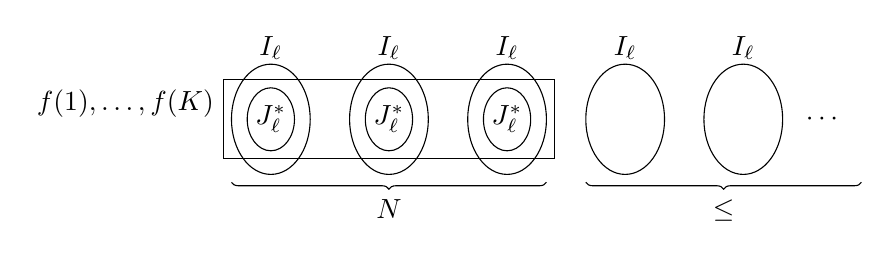
\begin{tikzpicture}
                          \foreach \x in {0,1.5,...,6} {
                                  \draw (\x,0) ellipse[x radius=0.5, y radius=0.7];
                                  \node at (\x,0.9) {$I_\ell$};
                              }
                          \foreach \x in {0,1.5,3} {
                                  \draw (\x,0) ellipse[x radius=0.3, y radius=0.4] node {$J^*_\ell$};
                              }
                          \node at (7,0) {$\cdots$};
                          \draw[decorate, decoration={brace, mirror}] (-0.5,-0.8) -- (3.5,-0.8) node[midway, below, yshift=-0.1cm] {$N$};
                          \draw[decorate, decoration={brace, mirror}] (4,-0.8) -- (7.5,-0.8) node[midway, below, yshift=-0.1cm] {$\leq \eps$};
                          \draw (-0.6,-0.5) rectangle (3.6,0.5);
                          \node[below left] at (-0.6,0.5) {$\mset{f(1),\dots,f(K)}$};
                      \end{tikzpicture}
                  \end{center}
                  Ziel ist es, zu jedem~$\eps$ hinreichend große~$N$ zu finden, sodass die Summe der ersten~$N$ Teilfamilien so groß wird, sodann der Rest kleiner~$\eps$ ist. Das können wir erreichen, indem wir hinreichend große endliche Teilmengen~$J^*_\ell \subset I_\ell$ betrachten, und darum eine größere Menge $\mset{f(1),\dots,f(K)}$ konstruieren, sodass $J^*_\ell \subset \mset{f(1),\dots,f(K)}$ für die ersten~$N$ Mengen~$J^*_\ell$. Da wir wissen, dass die Summe der~$(a_i)_{i\in I}$ mit $I \supset  \mset{f(1),\dots,f(K)}$ gegen~$a$ konvergiert, können wir dementsprechend~$N$ groß genug wählen.
              }\qedhere
    \end{enumerate}
\end{proof}

\begin{remark}
    Beide Umordnungssätze (\cref{thm:series:rearrangement,thm:family:rearrangement}) gelten auch ohne Voraussetzung der absoluten Konvergenz bzw.\ Summierbarkeit, falls alle~$a_i \geq 0$.

    Konvergiert die Reihe, so ist sie auch absolut konvergent. Divergiert die Reihe, so muss sie uneigentlich gegen~$\infty$ konvergieren. Das bedeutet aber, dass auch jede Umordnung uneigentlich gegen~$\infty$ konvergiert, denn andernfalls würe das dem Umordnungssatz widersprechen.

    Genauso lässt sich für die Summierbarkeit von Familien und deren Zerlegung in summierbare Teilfamilien argumentieren.
\end{remark}

\begin{corollary}[Doppelreihensatz]
    Sei $(a_{j\ell})_{(j,\ell)\in J\times L}$ eine summierbare Familie. Dann gilt
    \begin{equation*}
        \sum_{(j,\ell)\in J\times L} a_{j\ell} = \sum_{j\in J} \paren*{\sum_{\ell\in L} a_{j\ell}} = \sum_{\ell\in L} \paren*{\sum_{j\in J} a_{j\ell}},
    \end{equation*}
    d.\,h.\ die Summenzeichen lassen sich vertauschen.
\end{corollary}

\subsubsection{Beispiele für Umordnung}

\begin{proof}
    Wir verwenden den obigen Satz mit $I = J\times L$ und $I_\ell = J\times\mset{\ell}$. Dann ist $I = \dotbigcup_{\ell\in L} I_\ell$. Daraus folgt $\sum a_{j\ell} = \sum_{\ell\in L} (\sum_{j\in J} a_{j\ell})$. Vertauschen der Rollen von $J$~und~$L$ liefert die zweite Gleichheit.
\end{proof}

\begin{example}
    Für $J, L = \N_0$ definieren wir
    \begin{equation*}
        a_{j\ell} = \begin{cases}
            1  & \text{falls } j = 1,      \\
            -1 & \text{falls } j = \ell+1, \\
            0  & \text{sonst}.
        \end{cases}
    \end{equation*}
    Dann gilt $\sum_\ell \sum_j a_{j\ell} = 0$, aber $\sum_j \sum_\ell a_{j\ell} = +1$. Das ist auch offensichtlich, da $(a_{j\ell})_{(j,\ell)}$~nicht absolut summierbar ist!
\end{example}

\begin{example}
    Mit der geometrischen Reihe gilt
    \begin{equation*}
        \sum_{k=2}^\infty (\zeta(k)-1) = \sum_{k=2}^\infty \sum_{n=2}^\infty \frac{1}{n^k} = \sum_{n=2}^\infty \sum_{k=2}^\infty \frac{1}{n^k} = \sum_{n=2}^\infty \frac{1}{n(n-1)} = \sum_{n=2}^\infty \paren*{\frac{1}{n-1} - \frac{1}{n}}.
    \end{equation*}
\end{example}

\begin{notation}[Wahrscheinlichkeitsverteilung, Erwartungswert]
    Eine Folge~$(p_k)_{k\in\N_0}$ heißt \emph{Wahrscheinlichkeitsverteilung} auf~$N_0$, falls $p_k > 0$ für alle~$k$ und $\sum_{k=0}^\infty p_k = 1$.

    Als \emph{Erwartungswert} dieser Wahrscheinlichkeitsverteilung definieren wir $\mu = \sum_{k=0}^\infty kp_k$, falls dieser endlich ist bzw.\ konvergiert.
\end{notation}

\begin{theorem}
    Für den Erwartungswert gilt $\mu = \sum_{j=0}^\infty \paren*{\sum_{k>j} p_k}$.
\end{theorem}

\begin{proof}
    Wir setzen
    \begin{equation*}
        p_{jk} \coloneqq 1_{\mset{k>j}} p_k = \begin{cases}
            0 & \text{falls } k \leq j, \\
            1 & \text{falls } k > j.
        \end{cases} \quad\text{für } j,k \in \N_0.
    \end{equation*}
    Hierbei bezeichnet~$1_{\mset{k>j}}$ die sog.\ \emph{Indikatorfunktion} auf~$\mset{k > j}$. Dann gilt mit dem Doppelreihensatz mit~$p_k \geq 0$
    \begin{equation*}
        \mu = \sum_{k=0}^\infty kp_k = \sum_{k=0}^\infty \paren*{\sum_{j=0}^\infty p_{jk}} = \sum_{j=0}^\infty \paren*{\sum_{k=0}^\infty p_{jk}} = \sum_{j=0}^\infty \paren*{\sum_{k>j} p_k}. \qedhere
    \end{equation*}
\end{proof}

\begin{example}
    Für~$p \in (0, 1)$ definieren wir $p_k = p(1-p)^{k-1}$ für alle~$k \in \N$ und~$p_0 = 0$. Diese Verteilung gibt die Wahrscheinlichkeit, dass der $k$"~te Versuch zum ersten Mal zum Erfolg führt, an. Nun ist
    \begin{equation*}
        \sum_{k=0}^\infty = p \sum_{k=1}^\infty (1-p)^{k-1} = p \frac{1}{1-(1-p)} = 1,
    \end{equation*}
    also ist $p$~eine Wahrscheinlichkeitsverteilung. Des Weiteren ist
    \begin{equation*}
        \sum_{k=0}^\infty = kp_k = \sum_{j=0}^\infty \sum_{k=j+1}^\infty p(1-p)^{k-1} = \sum_{j=0}^\infty p\paren*{\frac{1}{1-(1-p)} - \frac{1-(1-p)^j}{1-(1-p)}} = \sum_{j=0}^\infty (1-p)^j = \frac{1}{p}.
    \end{equation*}

    \emph{Interpretation}: Bei einer Erfolgswahrscheinlichkeit~$p$ müssen wir im Mittel~$1/p$ Versuche durchführen, um einmal zu gewinnen.\footnote{Diese Verteilung ist als \emph{geometrische Verteilung} bekannt.}
\end{example}

\subsection{Produkte von Reihen}

\begin{definition}[diskrete Faltung]
    Für zwei reelle Folgen $(a_n)_{n\in\N_0}$ und $(b_n)_{n\in\N_0}$ definieren wir deren \emph{Faltung} als Folge~$(c_n)_{n\in\N_0}$ mit Glieder
    \begin{equation*}
        c_n \coloneqq (a*b)_n \coloneqq \sum_{k=0}^n a_k b_{n-k}.
    \end{equation*}

    Algemein für Familien $(a_n)_{n\in\Z}$ und $(b_n)_{n\in\Z}$ definieren wir
    \begin{equation*}
        (a*b)_n \coloneqq \sum_{k\in\Z} a_k b_{n-k}
    \end{equation*}
    (vorausgesetzt die Reihe konvergiert).
\end{definition}

\begin{theorem}[\textsc{Cauchy}-Produkt]\label{thm:cauchyprod}
    Sind $\sum a_n$ und~$\sum b_n$ absolut konvergente Reihen, so defineirt die Falutng der Folgenglieder eine absolut konvergente Reihe $\sum_n (a*b)_n$, genannt \emph{\textsc{Cauchy}-Produkt} der Reihen
    \begin{equation*}
        \paren*{\sum_{n=0}^\infty a_n} \paren*{\sum_{n=0}^\infty b_n} = \sum_{j,l=0}^\infty a_j b_l = \sum_{n=0}^\infty \paren*{\sum_{k=0}^n a_n b_{n-k}} = \sum_{n=0}^\infty (a*b)_n.
    \end{equation*}
\end{theorem}

\lecturesep{22.~November 2021}

\begin{center}
    \begin{tikzpicture}[scale=0.7]
        \draw[->] (0,0) -- (0,4) node[left] {$\N_0$};
        \draw[->] (0,0) -- (6,0) node[below] {$\N_0$};
        \foreach \x in {0,...,5} {
                \foreach \y in {0,...,3} {
                        \pic at (\x,\y) {dot};
                    }
            }
        \foreach \x in {1,...,7} {
            \draw ({min(\x,5)}, {max(0, \x-5)}) -- ({max(0,\x-3)}, {min(3,\x)});
        }
        \node[below left] at (0,0) {$a_0b_0$};
        \node[left] at (0,1) {$a_0b_1$};
        \node[below] at (1,0) {$a_1b_0$};
        \node[above, fill=white, yshift=0.5ex] at (1,1) {$a_1b_1$};
    \end{tikzpicture}
\end{center}

\begin{proof}
    Seien $A \coloneqq \sum_{j=0}^\infty \abs{a_j}$, $B \coloneqq \sum_{k=0}^\infty \abs{b_k}$, $a \coloneqq \sum_{j=1}^\infty a_j$ und $b \coloneqq \sum_{k=1}^\infty b_k$.

    Zuerst wollen wir zeigen, dass die Familie $(a_jb_k)_{(j,k)\in\N^2}$ summierbar ist. Für alle~$N \in \N$ gilt nämlich
    \begin{equation*}
        \sum_{j,k=0}^N \abs{a_jb_k} = \sum_{j=0}^N \paren*{\sum_{k=0}^N \abs{a_j}\cdot\abs{b_k}} \leq \sum_{j=0}^N \abs{a_j} B \leq AB < \infty.
    \end{equation*}

    Deshalb können wir den Doppelreihensatz anwenden und erhalten
    \begin{equation*}
        \sum_{(j,k) \in \N_0^2} a_jb_k = \sum_{j=0}^\infty \paren*{\sum_{k=0}^\infty a_jb_k} = \sum_{j=0}^\infty a_jb = ab.
    \end{equation*}

    Wir betrachten nun eine Zerlegung von $\N_0\times\N_0 = I = \dotbigcup_{\ell=0}^\infty I_\ell$ mit
    \begin{equation*}
        I_\ell \coloneqq \mset{(j,k) \in \N_0\times\N_0 : j+k=\ell} = \mset{(j,\ell-j) : j \in \mset{0, 1,\dots,\ell}},
    \end{equation*}
    also eine Zerlegung in geordneten Paaren mit vorgegebener Summe (den Geraden im Bild). Aus dem großen Umordnungssatz folgt
    \begin{equation*}
        \sum_{(j,k) \in \N_0^2} a_jb_k = \sum_{\ell=0}^\infty \sum_{(j,k)\in I_\ell} a_jb_k = \sum_{\ell=0}^\infty \sum_{j=0}^\ell a_jb_{\ell-j} = \sum_{\ell=0}^\infty (a*b)_{\ell}.
    \end{equation*}
    Damit sind der obige Ausdruck und $ab$ gleich der Summe der Familie.
\end{proof}

\subsubsection{Binomische Reihe}

\begin{theorem}[binomische Reihe]
    Für alle $x,\alpha \in \R$ mit~$\abs{x < 1}$ ist die Reihe
    \begin{equation*}
        B(x,\alpha) \coloneqq \sum_{n=0}^\infty \binom{\alpha}{n} x^n = 1 + \alpha x + \frac{\alpha(\alpha-1)}{1\cdot2} x^2 + \frac{\alpha(\alpha-1)(\alpha-2)}{1\cdot2\cdot3} x^3 + \cdots
    \end{equation*}
    absolut konvergent.
\end{theorem}

Die Summe ist endlich, falls~$\alpha \in \N$.

\begin{proof}
    Mit dem Quotientenkriterium folgt die Konvergenz der absoluten Reihe:
    \begin{equation*}
        \abs*{\frac{\abs{a_{n+1}}}{\abs{a_n}}} = \abs*{\frac{\abs{\alpha-n} \cdot \abs{x}}{n+1}} \xrightarrow{n\to\infty} \abs{x} < 1. \qedhere
    \end{equation*}
\end{proof}

\begin{lemma}
    Für alle $\alpha,\beta,x \in \R$ mit~$\abs{x} < 1$ gilt
    \begin{equation*}
        B(x,\alpha) \cdot B(x,\beta) = B(x,\alpha+\beta).
    \end{equation*}
\end{lemma}

\begin{proof}
    Es gilt für das Cauchy-Produkt (\cref{thm:cauchyprod})\footnote{Der Dozent verwendete hier die \emph{\textsc{chu}-\textsc{vandermondesche} Identität}, die wir noch nicht bewiesen haben. Führen wir das Symbol $\alpha^{[n]} \coloneqq \prod_{i=0}^n (\alpha-i)$ ein, können wir den Binomialkoeffizienten als $\binom{\alpha}{n} = \alpha^{[n]}/n!$ schreiben. Damit wird die Identität
        \begin{equation*}
            \frac{(\alpha+\beta)^{[n]}}{n!}= \binom{\alpha+\beta}{n} \overset{!}{=} \sum_{k=0}^n \binom{\alpha}{k}\binom{\beta}{n-k} = \sum_{k=0}^n \frac{\alpha^{[k]} \beta^{[n-k]}}{k!(n-k)!} \iff (\alpha+\beta)^{[n]} = \sum_{k=0}^n \binom{n}{k} \alpha^{[k]} \beta^{[n-k]}.
        \end{equation*}
        Das können wir analog zum normalen binomischen Lehrsatz via Induktion über~$n$ beweisen.}
    \begin{equation*}
        B(x,\alpha) \cdot B(x,\beta) = \sum_{n=0}^\infty \paren*{\sum_{k=0}^n \binom{\alpha}{k} x^k \binom{\beta}{n-k} x^{n-k}} = \sum_{n=0}^\infty \binom{\alpha+\beta}{n} x^n = B(x,\alpha+\beta). \qedhere
    \end{equation*}
\end{proof}

\begin{theorem}
    Für~$\alpha \in \Q^+$ und für~$x \in \R$ mit~$\abs{x} < 1$ gilt
    \begin{equation*}
        B(x,\alpha) = (1+x)^\alpha.
    \end{equation*}
\end{theorem}

\begin{proof}
    Sei~$\alpha = p/q$. Mit dem binomischen Lehrsatz sehen wir $(1+x)^p = B(x,p)$. Mit dem gerade bewiesenen Lemma erhalten wir $B(x,p) = B(x,q\alpha) = (B(x,\alpha))^q$, also $(1+x)^\alpha = (1+x)^{p/q} = B(x,\alpha)$.
\end{proof}

\section{Die Exponentialreihe}

\begin{definition}[Exponentialreihe, eulersche Zahl]
    Für alle~$x \in \R$ sei die \emph{Exponentialreihe}
    \begin{equation*}
        \exp(x) \coloneqq \sum_{n=0}^\infty \frac{x^n}{n!}.
    \end{equation*}

    Insbesondere ist die \emph{\textsc{eulersche} Zahl}
    \begin{equation*}
        e \coloneqq \exp(1) = \sum_{n=0}^\infty \frac{1}{n!} = 1 + 1 + \frac{1}{2} + \frac{1}{6} + \frac{1}{24} + \cdots \approx 2,7182818\dots
    \end{equation*}
\end{definition}

\subsection{Eigenschaften}

\begin{theorem}\leavevmode
    \begin{enumerate}
        \item Für alle~$x \in \R$ ist die Exponentialreihe absolut konvergent.
        \item Restgliedabschätzung: Für alle~$x \in \R$ und $N \in \N$ mit~$\abs{x} \leq 1+\frac{1}{2}N$ gilt
              \begin{equation*}
                  \abs*{\exp(x) - \sum_{n=0}^N \frac{x^n}{n!}} \leq 2 \frac{\abs{x}^{N+1}}{(N+1)!}.
              \end{equation*}
    \end{enumerate}
\end{theorem}

Die Restgliedabschätzung ist --~öfter als man denkt~-- nützlich, und lässt sich auch einfach merken: Der Rest ist kleiner als das doppelte des ersten Restglieds.

\begin{proof}\leavevmode
    \begin{enumerate}
        \item Nach dem Quotientenkriterium gilt
              \begin{equation*}
                  \abs*{\frac{a_{n+1}}{a_n}} = \frac{\abs{x}}{n+1} \xrightarrow{n\to\infty} 0.
              \end{equation*}
        \item Aus der Dreiecksungleichung und der geometrischen Reihe folgt
              \begin{align*}
                  \abs*{\exp(x) - \sum_{n=0}^N \frac{x^N}{n!}} & \leq \sum_{n=N+1}^\infty \frac{\abs{x}^n}{n!} = \frac{\abs{x}^{N+1}}{(N+1)!} \paren*{1 + \frac{\abs{x}}{N+2} + \frac{\abs{x}^2}{(N+2)(N+3)} + \cdots}                                                               \\
                                                               & \leq \frac{\abs{x}^{N+1}}{(N+1)!} \paren*{1 + \frac{\abs{x}}{N+2} + \frac{\abs{x}^2}{(N+2)^2} + \frac{\abs{x}^3}{(N+2)^3} + \cdots} = \frac{\abs{x}^{N+1}}{(N+1)!} \sum_{l=0}^\infty \paren*{\frac{\abs{x}}{N+2}}^l \\
                                                               & \leq 2\frac{\abs{x}^{N+1}}{(N+1)!}. \qedhere
              \end{align*}
    \end{enumerate}
\end{proof}

\begin{theorem}[Funktionalgleichung]
    Für alle $x,y \in \R$ gilt
    \begin{equation*}
        \exp(x) \cdot \exp(y) = \exp(x+y).
    \end{equation*}
\end{theorem}

\begin{proof}
    Mit dem Cauchy-Produkt für absolut konvergente Reihen und dem binomischen Lehrsatz gilt
    \begin{equation*}
        \exp(x) \cdot \exp(y) = \paren*{\sum_{n=0}^\infty \frac{x^n}{n!}} \paren*{\sum_{n=0}^\infty \frac{y^n}{n!}} = \sum_{n=0}^\infty \paren*{\sum_{k=0}^n \frac{x^k}{k!} \cdot \frac{y^{n-k}}{(n-k)!}} = \sum_{n=0}^\infty \frac{(x+y)^n}{n!} = \exp(x+y). \qedhere
    \end{equation*}
\end{proof}

\begin{remark}
    Die Exponentialfunktion~$\exp$ definiert einen Gruppenhomöomorphismus von der additiven Gruppe~$(\R,+)$ auf die multiplikative Gruppe~$((0,\infty),\cdot)$.
\end{remark}

\begin{corollary}\leavevmode
    \begin{enumerate}
        \item Für alle~$x \in \R$ gilt
              \begin{equation*}
                  \exp(x) > 0 \qquad\text{und}\qquad \exp(-x) = \frac{1}{\exp(x)}.
              \end{equation*}
        \item Für alle~$x \in \R$ und~$q \in \Q$ gilt
              \begin{equation*}
                  \exp(qx) = (\exp(x))^q.
              \end{equation*}
              Insebsondere folgt daraus auch $\exp(q) = e^q$.
    \end{enumerate}
\end{corollary}

\begin{proof}\leavevmode
    \begin{enumerate}
        \item Aus der Funktionalgleichung folgt
              \begin{equation*}
                  \exp(x) = \exp\paren*{\frac{x}{2}} \exp\paren*{\frac{x}{2}} = \paren*{\exp\paren*{\frac{x}{2}}}^2 \geq 0.
              \end{equation*}
              Ferner gilt $\exp(x) \neq 0$, denn für alle~$x \in \R$ gilt $1 = \exp(0) = \exp(x) \cdot \exp(-x)$, und aufgrund Nullteilerfreiheit ist keiner der Faktoren Null.

              Ferner folgt daraus $1/\exp(x) = \exp(-x)$.
        \item Wir beweisen zuerst $\exp(nx) = (\exp(x))^n$ für natürliche~$n$. Der Anfang~$n = 1$ ist klar. Der Schritt:
              \begin{equation*}
                  \exp((n+1)x) = \exp(x) \cdot \exp(nx) = \exp(x) \cdot \exp(x)^n = (\exp(x))^{n+1}.
              \end{equation*}
              Ferner gilt
              \begin{equation*}
                  \exp(-nx) = \frac{1}{\exp(nx)} = \frac{1}{(\exp(x))^n} = \exp(x)^{-n},
              \end{equation*}
              also gilt die Gleichung auch für alle ganzen Zahlen. Schließlich erhalten wir für alle~$q = k/m$, $k \in \Z$ und~$m \in \N$
              \begin{equation*}
                  (\exp(qx))^m = \exp(mqx) = \exp(kx) = (\exp(x))^k \implies \exp(qx) = (\exp(x))^{k/m} = (\exp(x))^q. \qedhere
              \end{equation*}
    \end{enumerate}
\end{proof}

\begin{proposition}\label{prop:exponential:estimate}\leavevmode
    \begin{enumerate}
        \item Es gilt $\exp(x) \geq 1+x$ für alle~$x \in \R$.
        \item Es gilt $\exp(x) \leq 1/(1-x)$ für alle~$x < 1$.
    \end{enumerate}
\end{proposition}

\begin{proof}\leavevmode
    \begin{enumerate}
        \item Für~$x \geq 0$ gilt natürlich $\sum_{n=0}^\infty x^n/n! \geq 1+x$.

              Für~$x < 0$ betrachten wir $\exp(-x)$ mit~$x > 0$. Für~$\abs{x} < 1$ ist $\exp(-x) = \sum_{n=0}^\infty (-x)^n/n!$ nach dem Leibniz-Kriterium konvergent, denn die Reihe ist alternierend, der Betrag~$x^n/n!$ ist monoton fallend und konvergiert gegen Null. Aus dem \emph{Beweis} des Leibniz-Kriteriums (s.~\cref{thm:series:leibniz}) geht hervor, dass für die Partialsummen~$s_{2n-1} \geq s_1$ für alle~$n \geq 1$ gilt, also auch $\exp(-x) \geq s_1 = 1-x$.

              Diese Abschätzung gilt auch für~$x \geq 1$, denn es gilt stets~$\exp(-x) > 0$, aber $1-x \leq 0$. Schließlich erhalten wir $\exp(-x) \geq 1-x$ für alle~$x > 0$, also $\exp(x) \geq 1+x$ für alle~$x \in \R$.
        \item Das folgt aus $\exp(-x) \geq 1-x$ durch Kehrwertbildung:
              \begin{equation*}
                  \exp(x) = \frac{1}{\exp(-x)} \leq \frac{1}{1-x},
              \end{equation*}
              gültig für alle~$x < 1$.\qedhere
    \end{enumerate}
\end{proof}

\begin{center}
    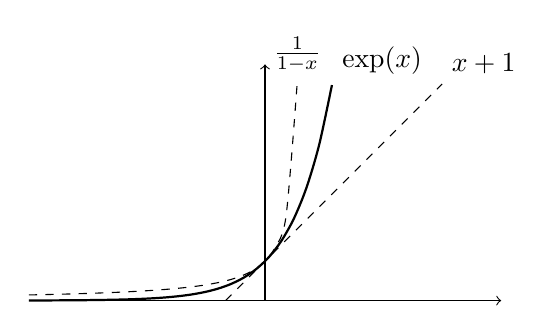
\begin{tikzpicture}[scale=0.5]
        \draw[->] (-6,0) -- (6,0);
        \draw[->] (0,0) -- (0,6);

        \draw[domain=-6:1.7, smooth, thick] plot (\x,{exp(\x)}) node[above right] {$\exp(x)$};
        \draw[domain=-1:4.5, smooth, dashed] plot (\x,{\x+1}) node[above right] {$x+1$};
        \draw[domain=-6:0.82, smooth, dashed] plot (\x,{1/(1-\x)}) node[above] {$\frac{1}{1-x}$};
    \end{tikzpicture}
\end{center}

\subsection{Grenzwertdarstellung}

\begin{theorem}[Grenzwertdarstellung der Exponentialfunktion]
    Für alle~$x \in \R$ gilt
    \begin{equation*}
        \lim_{n\to\infty} \paren*{1+\frac{x}{n}}^n = \exp(x).
    \end{equation*}
    Insebsondere gilt $e = \lim_{n\to\infty} (1+1/n)^n$.
\end{theorem}

Der obige Satz impliziert auch, dass $\lim_{n\to\infty} (1+x/n)^n$ existiert.

\begin{proof}
    Zuerst betrachten wir den Fall~$x \geq 0$. Nach dem binomischen Lehrsatz gilt für alle~$n \in \N$ mit $x \geq 0$
    \begin{equation*}
        \paren*{1+\frac{x}{n}}^n = \sum_{k=0}^n \binom{n}{k} \frac{x^k}{n^k} = 1 + \sum_{k=1}^n \frac{x^k}{k!} \cdot \underbrace{\frac{n(n-1)\cdots(n-k+1)}{n\cdot n\cdots n}}_{k\text{ Faktoren}, \leq 1} \leq 1 + \sum_{k=1}^\infty \frac{x^k}{k!} = \exp(x).
    \end{equation*}
    Umgekehrt gilt mit dem binomischen Lehrsatz für alle~$n \geq m$ mit~$x \geq 0$
    \begin{equation*}
        \paren*{1+\frac{x}{n}}^n = \sum_{k=0}^n \binom{n}{k} \frac{x^k}{n^k} \geq \sum_{k=0}^m \frac{x^k}{k!} \paren*{\frac{n}{n}\cdot\frac{n-1}{n}\cdots\frac{n-k+1}{n}} \xrightarrow{n\to\infty} \sum_{k=0}^m \frac{x^k}{k!} \cdot 1.
    \end{equation*}
    (\emph{Achtung}: Wir haben in der obigen Abschätzung nur bis~$m$ summiert.) Das bedeutet nach dem Satz von Bolzano-Weierstraß
    \begin{equation*}
        \liminf_{n\to\infty} \paren*{1+\frac{x}{n}}^n \geq \sum_{k=0}^m \frac{x^k}{k!} \quad\text{für jedes } m \in \N.
    \end{equation*}
    Lassen wir nun $m \to \infty$, erhalten wir
    \begin{equation*}
        \liminf_{n\to\infty} \paren*{1+\frac{x}{n}}^n \geq \sum_{k=0}^\infty \frac{x^k}{k!} = \exp(x).
    \end{equation*}
    Zusammen erhalten wir für alle~$x \geq 0$
    \begin{equation*}
        \lim_{n\to\infty} \paren*{1+\frac{x}{n}}^n = \exp(x).
    \end{equation*}

    Nun zum Fall~$x < 0$ bzw.\ $\exp(-x)$ für~$x > 0$. Für~$x > 0$ und hinreichend große~$n$ gilt
    \begin{equation*}
        0 \leq \paren*{1+\frac{x}{n}} \paren*{1-\frac{x}{n}} = 1 - \paren*{\frac{x}{n}}^2 \leq 1.
    \end{equation*}
    Mit $1+x/n > 0$ und der Ordnungserhaltung unter $\limsup$ folgt daraus\footnote{Hier wurde ein Lemma verwendet, dass wir noch nicht bewiesen haben: Sei $A \subset \R$ eine nach unten beschränkte Menge und $f\colon \mset{\inf A} \cup A \to \R$ eine monoton (schwach) fallende Abbildung. Dann gilt $\sup f(A) \leq f(\inf A)$. \emph{Beweis}: Angenommen $\sup f(A) > f(\inf A)$. Weil das Supremum die kleinste obere Schranke ist, gibt es ein~$a \in A$ mit $f(a) > f(\inf A)$. Aus der Monotonie folgt aber $a \leq \inf A$, also $a = \inf A = \min A$. Aus der Monotonie folgt aber auch $\sup f(A) = f(\min A) = f(\inf A)$, Widerspruch.}
    \begin{equation*}
        \limsup_{n\to\infty} \paren*{1-\frac{x}{n}}^n \leq \limsup_{n\to\infty} \frac{1}{(1+x/n)^n} \leq \frac{1}{\liminf_{n\to\infty} (1-x/n)^n} = \frac{1}{\exp(x)} = \exp(-x).
    \end{equation*}

    Ferner gilt für alle~$x > 0$: Für jedes~$\eps > 0$ gibt es hinreichend große~$n$, sodass
    \begin{equation*}
        \paren*{1+\frac{x+\eps}{n}} \paren*{1-\frac{x}{n}} = 1 + \frac{\eps}{n} - \frac{x(x+\eps)}{n^2} \geq 1
    \end{equation*}
    (z.\,B.\ für alle~$n \geq n_0$ mit $\eps n_0 \geq x(x+\eps)$). Daraus folgt wie oben mit der Ordnungserhaltung von $\liminf$
    \begin{equation*}
        \liminf_{n\to\infty} \paren*{1-\frac{x}{n}}^n \geq \liminf_{n\to\infty} \frac{1}{(1 + (x+\eps)/n)^n} = \lim_{n\to\infty} \frac{1}{(1 + (x+\eps)/n)^n} = \frac{1}{\exp(x+\eps)} = \exp(-x-\eps),
    \end{equation*}
    wobei wir beim Übergang von $\liminf$ auf~$\lim$ ausgenutzt haben, dass der Bruch (für $x+\eps \geq 0$) konvergiert. Nun folgt aus der Funktionalgleichung und \cref{prop:exponential:estimate}
    \begin{equation*}
        \exp(-x-\eps) = \exp(-x) \cdot \exp(-\eps) \geq \exp(-x) (1-\eps).
    \end{equation*}
    Schließlich\footnote{Vor diesem Schritt schätzte der Dozent $\exp(-x) \cdot \exp(-\eps) \geq \exp(-x) (1-2\eps)$ ab und verwendete die Restgliedabschätzung nach dem $N = 0$"~ten Glied, was $\abs{\exp(x) - 1} \leq 2\eps$ ergibt. Meiner Meinung nach ist das aber nicht nötig.} erhalten wir für jedes~$\eps > 0$
    \begin{equation*}
        (1-\eps) \exp(-x) \leq \liminf \paren*{1-\frac{x}{n}}^n \leq \limsup \paren*{1-\frac{x}{n}}^n \leq \exp(-x) \implies \lim_{n\to\infty} \paren*{1-\frac{x}{n}}^n = \exp(-x). \qedhere
    \end{equation*}
\end{proof}

\lecturesep{24.~November 2021}

\begin{example}
    Sei $x$~ein Zinssatz bei jährlicher Anlage, $x/2$~bei halbjähriger Anlage, $x/12$~bei monatlicher, $x/365$~bei täglicher Anlage, usw. Das Kapital~$K_0$ nach einem Jahr wäre dann
    \begin{equation*}
        K_0(1+x), \quad K_0\paren*{1+\frac{x}{2}}^2, \quad K_0\paren*{1+\frac{x}{12}}^{12}, \quad K_0\paren*{1+\frac{x}{365}}^{365}, \quad \ldots, \quad K_0 \exp(x).
    \end{equation*}
    Für bspw.~$x = 1$ erhalten wir
    \begin{equation*}
        2K_0; \quad 2,25K_0; \quad \ldots; \quad (2,718\ldots)K_0.
    \end{equation*}
\end{example}

\section{Komplexe Zahlen}

\subsection{Motivation und Definition}

Eine Möglichkeit, um die \emph{komplexen Zahlen}~$\C$ zu konstruieren, ist über folgende \emph{Körpererweiterung} von~$\R$ nach~$\C$.

Angenommen es gibt einen Körper~$K$, der $\R$~enthält (aber nicht notwendigerweise alle Eigenschaften von~$\R$ hat) und ein Element~$i$ mit~$i^2 = -1$ enthält.

Dann sind aufgrund Abgeschlossenheit von~$K$ für $x,y,u,v \in \R \subset \C$ auch $(x+iy) \in K$ und $(u+iv) \in K$ mit
\begin{equation*}
    (x+iy) + (u+iv) = (x+u) + i(y+v) \qquad\text{und}\qquad (x+iy) \cdot (u+iv) = (xu-yv) + i(yu+xv).
\end{equation*}
Damit ist die Menge $K_0 \coloneqq \mset{x+iy : x,y \in \R}$ abgeschlossen bzgl.\ Addition~$+$ und Multiplikation~$\cdot$, es gibt $0, 1 \in K_0$ und $K_0$~ist abgeschlossen unter additive und multiplikative Inversenbildung. Diesen Körper~$K_0$ bezeichnen wir mit~$\C$.

Wir wollen es aber "`von Hinten"' aufziehen und nicht die Existenz eines solchen Körpers zuerst voraussetzen (da wir es mit unserem Kenntnisstand noch nicht wissen).

\begin{theorem}[Körper der komplexen Zahlen]\label{thm:complexnumbers}
    Die Menge $\R\times\R = \mset{(x,y) : x,y \in \R}$ der geeordneten Paare reller Zahlen definiert einen \emph{Körper} mit \emph{Addition} und \emph{Multipikaiton}, definiert durch
    \begin{equation*}
        (x,y) + (u,v) \coloneqq (x+u,y+v) \qquad\text{und}\qquad (x,y) \cdot (u,v) \coloneqq (xu-yv,yu+xv),
    \end{equation*}
    \emph{neutrale Elemente} $0 \coloneqq (0, 0)$, $1 \coloneqq (1, 0)$ sowie \emph{Inverse}, definiert durch
    \begin{equation*}
        -(x,y) \coloneqq (-x,-y) \qquad\text{und}\qquad (x,y)^{-1} \coloneqq \paren*{\frac{x}{x^2+y^2},\frac{-y}{x^2+y^2}} \quad\text{falls } (x,y) \neq (0, 0)
    \end{equation*}
    mit $x,y,u,v \in \R$.
\end{theorem}

\begin{proof}
    Der Nachweis ist wirklich nur stures nachrechnen, weshalb wir uns hier sehr kurz fassen.
    \begin{itemize}
        \item Gruppenstruktur bzgl.\ Addition: trivial.
        \item Gruppenstruktur bzgl.\ Multiplikation:
              \begin{itemize}
                  \item Kommutativität: $(x,y) \cdot (u,v) = (xu-yv,yu+xv) = (ux-vy,uy+vx) = (u,v) \cdot (x,y)$, wobei wir für die mittlere Gleichheit die Kommutativität in~$\R$ nutzten.
                  \item Neutrales Element: $(x,y) \cdot (1, 0) = \cdots = (x,y)$.
                  \item Inverses:
                        \begin{equation*}
                            (x,y) \cdot \paren*{\frac{x}{x^2+y^2},\frac{-y}{x^2+y^2}} = \cdots = \paren*{\frac{x^2+y^2}{x^2+y^2},\frac{-xy+yx}{x^2+y^2}} = (1, 0).
                        \end{equation*}
                  \item Assoziativität: $(x,y) \cdot ((u,v) \cdot (s,t)) = \cdots = ((x,y) \cdot (u,v)) \cdot (s,t)$.
                  \item Distributivität: $(x,y) ((u,v) + (s,t)) = \cdots = (x,y)\cdot(u,v) + (x,y)\cdot(s,t)$.\qedhere
              \end{itemize}
    \end{itemize}
\end{proof}

Wir beobachten: Für~$(x, 0)$ und~$(u, 0)$ mit $x,u \in \R$ gilt
\begin{equation*}
    (x, 0) + (u, 0) = (x+u, 0) \qquad\text{sowie}\qquad (x, 0) \cdot (u, 0) = (xu, 0).
\end{equation*}
Deshalb bildet $\mset{(x,y) \in \C : y = 0}$ einen \emph{Teilkörper} von~$\C$, der \emph{isomoprh} zu~$\R$ ist. Daher identifizieren wir $\R$ mit $\mset{(x, 0) : x \in \R} \subset \C$ und schreiben $x = (x, 0) \in \C$ für alle~$x \in \R$. Damit ist~$\R \subset \C$.

Ferner setzen wir $i \coloneqq (0, 1)$, woraus $i^2 = (0, 1)\cdot(0, 1) = (-1, 0) = -1 \in \R$ sowie
\begin{equation*}
    (x,y) = (x, 0)+(0,y) = x(1, 0)+y(0, 1) = x+iy
\end{equation*}
für alle $x,y \in \R$ folgt. Damit können wir den Körper der komplexen Zahlen definieren.

\begin{definition}[Körper der komplexen Zahlen, imaginäre Einheit, Real"~\slash Imaginärteil]
    Wir setzen den Körper aus \cref{thm:complexnumbers} vor. Sei $i \coloneqq (0, 1)$ mit~$i^2 = -1$ die \emph{imaginäre Einheit}. Dann lässt sich jede \emph{komplexe Zahl} des Körpers schreiben als $z = (x,y) = x+iy$ mit \emph{Realteil} $\real(z) = x$ und \emph{Imaginärteil} $\imag(z) = y$ von~$z$.
    \begin{equation*}
        \C \coloneqq \mset{x+iy : x,y \in \R}
    \end{equation*}
    heißt \emph{Körper der komplexen Zahlen}.
\end{definition}

\emph{Achtung}: Der Imaginärteil $\imag(z)$ einer komplexen Zahl~$z$ sollte nicht mit dem Bild $\mathrm{im}(z)$ einer Abbildung~$z$ verwechselt werden.

Die komplexen Zahlen lassen sich gut in einer $\R\times\R$"~Ebene, einem kartesischen Koordinatensystem visualisieren, der sog.\ \emph{komplexen} bzw.\ \emph{\textsc{gaußschen} Zahlenebene}.

\begin{figure}
    \begin{tikzpicture}
        \draw[->] (-4,0) -- (4,0) node[below] {$\R$};
        \draw[->] (0,-4) -- (0,4) node[left] {$i\R$};

        \foreach \i in {-3,-2,-1,1,2,3} {
                \pic at (0,\i) {ytick=$\i i$};
                \pic at (\i,0) {xtick=$\i$};
            }
        \draw (0,0) -- (-2,1) pic {dot} node[left] {$w=u+iv$};
        \draw (0,0) -- (3,2) pic {dot} node[right] {$z=x+iy$};
        \draw (0,0) -- (1,3) pic {dot} node[above] {$w+z$};
        \draw (0,0) -- (3,-2) pic {dot} node[below] {$\conj{z}$};
    \end{tikzpicture}
    \caption{Komplexe Zahlenebene.}
\end{figure}

Dabei entspricht
\begin{itemize}
    \item $\C$~der Ebene,
    \item $\R$~der $x$"~Achse (also dem reellen "`Zahlenstrahl"') und
    \item $i\R = \mset{ix : x \in \R}$, die rein \emph{imaginären Zahlen} der $y$"~Achse.
\end{itemize}
Addition zweier komplexer Zahlen entspricht der Addition zweier Vektoren in~$\R^2$ (indem wir einen der Pfeile an die Spitze des anderen Pfeils verschieben~-- die Spitze des ersten Pfeils ist die Summe). Die Multiplikation funktioniert aber doch etwas anders~\dots

\subsection{Komplexe Konjugation und Betrag}

\begin{definition}[komplexe Konjugation]
    Die Abbildung $\conj{\cdot}\colon \C \to \C$ mit
    \begin{equation*}
        z = (x+iy) \mapsto \conj{z} = (x-iy)
    \end{equation*}
    ist die \emph{komplexe Konjugation}. $\conj{z}$~ist die \emph{komplex Konjugierte} von~$z$.
\end{definition}

In der komplexen Zahlenebene entspricht die Konjugation der Spiegelung an der $x$"~Achse.

\begin{lemma}[Rechenregeln mit Konjugierten]
    Für die Konjugation gilt mit $z = x+iy \in \C$ und~$w \in \C$:
    \begin{enumerate}
        \item $\conj{\conj{z}} = z$.
        \item $\conj{z+w} = \conj{z}+\conj{w}$.
        \item $\real(z) = \frac{1}{2}(z+\conj{z})$ und $\imag(z) = \frac{1}{2}(z-\conj{z})$.
        \item $z\conj{z} = x^2+y^2$, also ist $z\conj{z}$~reell und~$\geq 0$. Ferner ist $z\conj{z} = 0$ genau dann, wenn $z = 0$.\footnote{Eine weitere (wie ich finde) nützliche Regel: Für~$a \in \R$ und~$z \in \C$ gilt $\conj{az} = a\conj{z}$.}
    \end{enumerate}
\end{lemma}

\begin{proof}
    Das erfolgt durch einfaches nachrechnen.
\end{proof}

\begin{definition}[Betrag]
    Der Betrag einer komplexen Zahl $z = x+iy \in \C$ ist
    \begin{equation*}
        \abs{z} \coloneqq \sqrt{z\conj{z}} = \sqrt{x^2+y^2}.
    \end{equation*}
\end{definition}

\begin{figure}
    \begin{tikzpicture}[scale=0.7]
        \draw[->] (0,0) -- (5,0);
        \draw[->] (0,0) -- (0,4);

        \draw[dashed] (4,0) node[below] {$x$} |- (0,3) node[left] {$y$};
        \draw (0,0) -- node[near end, left] {$\sqrt{x^2+y^2}$} (4,3) pic {dot} node[right] {$z=x+iy$};
    \end{tikzpicture}
    \caption{Geometrische Visualisierung des Betrags.}
\end{figure}

\begin{lemma}[Rechenregeln mit Beträgen]\label{lem:complex:absolute}
    Für Beträge gilt mit $z = x+iy \in \C$ und~$w \in \C$:
    \begin{enumerate}
        \item $\abs{z} \geq 0$, und $\abs{z} = 0$ genau dann, wenn $z = 0$.
        \item $\abs{z} = \abs{\conj{z}}$.
        \item $\abs{\real(z)} \leq \abs{z}$ und $\abs{\imag(z)} \leq \abs{z}$.
        \item $\abs{z+w} \leq \abs{z}+\abs{w}$ \emph{(Dreiecksungleichung)}.
        \item $\abs{zw} = \abs{z}\cdot\abs{w}$.
        \item $1/z = \conj{z}/\abs{z}$ für~$z \neq 0$.
    \end{enumerate}
\end{lemma}

\begin{figure}
    \begin{tikzpicture}[scale=0.7]
        \draw[->] (0,0) -- (0,2.5);
        \draw[->] (0,0) -- (4,0);

        \draw (0,0) -- (1,1.5) pic {dot} node[above] {$w$};
        \draw 
            (0,0) -- (2,0.5) pic {dot} node[right] {$z$}
            -- (3,2) pic {dot} node[right] {$z+w$} -- cycle;
    \end{tikzpicture}
    \caption{Geomtrische Visualisierung der Dreiecksungleichung.}
\end{figure}

\begin{proof}
    Die Beweise folgen direkt aus den Definitionen. Deshalb zeigen wir hier nur eine Auswahl an Aussagen.
    \begin{enumerate}[start=2]
        \item Es gilt $\abs{z} = \sqrt{z\conj{z}} = \sqrt{\conj{z}z} = \abs{\conj{z}}$.
        \item Für $z = x+iy$ gilt $\abs{z}^2 = \real(z)^2 + \imag(z)^2 \geq \real(z)^2$. Analog für $\imag(z)^2$.
        \item Es gilt
              \begin{multline*}
                  \abs{z+w}^2 = (z+w)(\conj{z}+\conj{w}) = z\conj{z} + (z\conj{w} + \conj{z}w) + w\conj{w} = \abs{z}^2 + 2\real(z\conj{w}) + \abs{w}^2 \\
                  \leq \abs{z}^2 + 2\abs{z\conj{w}} + \abs{w}^2 = \abs{z}^2 + 2\abs{zw} + \abs{w}^2 = (\abs{z}+\abs{w})^2.
              \end{multline*}
              Anschließendes Wurzelziehen ergibt die Behauptung, wobei Beträge stets nicht-negativ sind.\qedhere
    \end{enumerate}
\end{proof}

\lecturesep{29.~November 2021}

\begin{remark}\leavevmode
    \begin{enumerate}
        \item Auf~$\C$ können wir keine Ordnung einführen, denn aus den Ordnungsaxiomen würde $z^2 \geq 0$ für alle~$z \in \C$ folgen. Das steht aber im Widerspruch zu~$i^2+1 = 0$ denn eine nicht-negative Zahl plus eine positive Zahl kann nicht Null ergeben.
        \item Falls wir~$z \geq 0$ schreiben, so meinen wir stets: "`$z \in \R$ und~$z \geq 0$"'.
        \item Im Allgemeinen gilt \underline{nicht} $z^2 = \abs{z}^2$ (z.\,B.\ $i^2 = -1 \neq 1 = \abs{i}^2$).
    \end{enumerate}
\end{remark}

\subsection{Folgen in~\texorpdfstring{$\C$}{C}}

\begin{definition}[komplexe Folge]
    Sei $(c_n)_{n\in\N}$ eine Folge in~$\C$.
    \begin{enumerate}
        \item Die Folge \emph{konvergiert gegen~$c \in \C$}, falls es für jedes~$\eps > 0$ ein~$N \in \N$ gibt, sodass $\abs{c_n-c} \leq \eps$ für alle~$n \geq N$ gilt. In Zeichen:
              \begin{equation*}
                  \forall \eps \geq 0\colon \exists N \in \N\colon \forall n \geq N\colon \abs{c_n-c} \leq \eps.
              \end{equation*}
        \item Die Folge ist eine \emph{\textsc{Cauchy}-Folge}, falls es für jedes~$\eps > 0$ ein~$N \in \N$ gibt, sodass $\abs{c_n-c_m} \leq \eps$ für alle~$n,m \geq N$ gilt. In Zeichen:
              \begin{equation*}
                  \forall \eps \geq 0\colon \exists N \in \N\colon \forall n,m \geq N\colon \abs{c_n-c_m} \leq \eps.
              \end{equation*}
    \end{enumerate}
\end{definition}

Die Definition für komplexe Folgen sind \emph{identisch} zu den Definition für reelle Folgen, wobei wir hier beachten sollten, das eine etwas andere Betragsdefinition gilt (vgl.\ \cref{def:convergence,def:cauchysequence}).

\begin{figure}
    \begin{tikzpicture}
        \draw[->] (0,0) -- (3,0);
        \draw[->] (0,0) -- (0,3);
        \coordinate[label=above left:$c$] (c) at (2,2);
        \coordinate[label=right:$c_{N-1}$] (cn1) at (2.3,0.8);
        \coordinate[label=above:$c_N$] (cn) at (2.3,1.2);
        \foreach \name in {c,cn1,cn} {
                \pic at (\name) {dot};
            }
        \draw (c) circle[radius=1];
        \draw (c) -- ++(45:1) node[midway, above left] {$\eps$};
        \foreach \x/\y in {0.3/0.8,0.5/1.6,1/0.3,0.9/2.6,1.7/0.8} {
                \pic at (\x,\y) {dot};
            }
        \foreach \a/\r in {-135/0.3,0/0.5,20/0.8,100/0.6,-100/0.8,170/0.6,-175/0.7} {
                \pic at ([shift=(c)]\a:\r) {dot};
            }
    \end{tikzpicture}
    \caption{Visualisierung des Konvergenzbegriffs in der komplexen Zahlenebene.}
\end{figure}

\subsubsection{Cauchy-Folgen}

\begin{theorem}[Konvergenz in~$\C$, komplexe Cauchy-Folgen]
    Sei $(c_n)_n$~eine komplexe Zahlenfolge mit $c_n = a_n+ib_n$, d.\,h.\ $a_n = \real(c_n)$, $b_n = \imag(c_n)$.
    \begin{enumerate}
        \item $(c_n)_n$~konvergiert genau dann gegen~$c = a+ib$, wenn $(a_n)_n$ gegen~$a = \real(c) \in \R$ \underline{und} $(b_n)_n$ gegen~$b = \imag(c) \in \R$ konvergiert. (Eine komplexe Folge konvergiert genau dann, wenn die Folgen der Real"~ und Imaginärteile konvergieren.)
        \item $(c_n)_n$~ist genau dann eine Cauchy-Folge in~$\C$, wenn $(a_n)_n$~\underline{und}~$(b_n)_n$ Cauchy-Folgen sind.
    \end{enumerate}
\end{theorem}

D.\,h.\ wir können sehr leicht mit komplexen Zahlenfolgen umgehen, wenn wir die Real"~ und Imaginärteile getrennt betrachten.

\begin{proof}\leavevmode
    \begin{enumerate}
        \item Sei $c_n \to c$ in~$\C$, d.\,h.\ dass es zu jedem~$\eps > 0$ ein~$N \in \N$ existiert, sodass $\abs{c_n-c} \leq \eps$ für alle~$n \geq N$ gilt. Aus \cref{lem:complex:absolute} folgt für alle~$n \geq N$ dann
              \begin{equation*}
                  \abs{a_n-a} = \abs{\real(c_n-c)} \leq \abs{c_n-c} \leq \eps.
              \end{equation*}
              Damit konvergiert $(a_n)_n$ gegen~$a \in \R$. Analog gilt für alle~$n \geq N$
              \begin{equation*}
                  \abs{b_n-b} = \abs{\imag(c_n-c)} \leq \abs{c_n-c} \leq \eps,
              \end{equation*}
              also konvergiert auch $(b_n)_n$ gegen~$b \in \R$.

              Für die Hinrichtung seien $a_n \to a$ und $b_n \to b$. Für jedes~$\eps > 0$ gibt es also ein~$N_a \in \N$, sodass $\abs{a_n-a} \leq \eps$ für alle~$n \geq N_a$ gilt, und ein~$N_b \in \N$, sodas $\abs{b_n-b} \leq \eps$ für alle~$n \geq N_b$ gilt. Setzen wir nun $N \coloneqq \max\mset{N_a,N_b}$, dann gilt mit der Betragsdefinition für alle~$n \geq N$
              \begin{equation*}
                  \abs{c_n-c}^2 = \abs{a_n-a}^2 + \abs{b_n-b}^2 \leq 2\eps \implies \abs{c_n-c} \leq \sqrt{2\eps}.
              \end{equation*}
              Damit konvergiert~$(c_n)_n$ gegen~$c \in \C$.
        \item Der Beweis erfolgt identisch, indem wir $c$~durch~$c_m$ an jeder Stelle des Beweises ersetzen.\qedhere
    \end{enumerate}
\end{proof}

\begin{corollary}[Vollständigkeit von~$\C$]
    $\C$~ist vollständig, denn jede Cauchy-Folge in~$\C$ konvergiert.
\end{corollary}

\begin{proof}
    Da die Cauchy-Folgen $(\real(c_n))_n$ und $(\imag(c_n))_n$ in~$\R$ konvergieren, konvergiert auch die Cauchy-Folge~$(c_n)_n$ mit $c_n = \real(c_n)+i\imag(c_n)$ in~$\C$.
\end{proof}

\subsubsection{Grenzwertsätze}

\begin{corollary}[Grenzwertsätze in~$\C$]
    Für zwei komplexe Folgen $c_n \to c$ und $d_n \to d$ gilt
    \begin{equation*}
        \lim_{n\to\infty} (c_n+d_n) = \lim_{n\to\infty} c_n + \lim_{n\to\infty} d_n = c+d \qquad\text{und}\qquad \lim_{n\to\infty} (c_nd_n) = \paren*{\lim_{n\to\infty} c_n} \paren*{\lim_{n\to\infty} d_n} = cd,
    \end{equation*}
    und, falls $d_n \neq 0$ und~$d \neq 0$ für alle~$n \geq N$ mit hinreichend großem~$N$,
    \begin{equation*}
        \lim_{n\to\infty} \frac{c_n}{d_n} = \frac{\lim_{n\to\infty} c_n}{\lim_{n\to\infty} d_n} = \frac{c}{d}.
    \end{equation*}
\end{corollary}

\begin{proof}
    Die Summe und das Produkt der komplexen Folgen lässt sich umschreiben zu
    \begin{align*}
        c_n+d_n & = (\real(c_n)+\real(d_n)) + i(\imag(c_n)+\imag(d_n))                                          &  & \text{und} \\
        c_nd_n  & = (\real(c_n)\real(d_n)-\imag(c_n)\imag(d_n)) + i(\real(c_n)\imag(d_n)+\imag(c_n)\real(d_n)).
    \end{align*}
    Damit konnten wir die Konvergenz der neuen Folgen auf die Konvergenz reeller Folgen zurückführen.

    Für den Quotienten gilt
    \begin{equation*}
        \frac{c_n}{d_n} = \frac{c_n\conj{d_n}}{\abs{d_n}^2},
    \end{equation*}
    woraus auch wieder die Konvergenz der komplexen Folge folgt, da die Real"~ und Imaginärteile wieder aus Summe, Produkte und Quotienten konvergenter reeller Folgen bestehen.
\end{proof}

\begin{corollary}[Konjugation einer konvergenten Folge]\label{cor:complex:sequence:conjugate}
    Mit~$(c_n)_n$ ist auch $(\conj{c_n})_n$ eine komplexe Cauchy-Folge und aus $c_n \to c$ folgt $\conj{c_n} \to \conj{c}$. Oder mit anderen Worten
    \begin{equation*}
        \lim_{n\to\infty} \conj{c_n} = \conj{\lim_{n\to\infty} c_n.}
    \end{equation*}
\end{corollary}

\begin{proof}
    Es gilt $\conj{c_n} = \real(c_n)-i\imag(c_n)$ und $\conj{c} = \real(c)-i\imag(c)$.
\end{proof}

\begin{corollary}[Betrag einer konvergenten Folge]
    Gilt für eine komplexe Folge $c_n \to c$, so gilt auch $\abs{c_n} \to \abs{c}$.
\end{corollary}

Die Umkehrung gilt hingegen (wie in den reellen Zahlen) \underline{nicht}.

\begin{proof}
    Es gilt $\abs{c_n} = \sqrt{\real(c_n)+\imag(c_n)}$ und $\abs{c} = \sqrt{\real(c)+\imag(c)}$. Damit ist $\abs{c_n}$~eine reelle Folge und wir können die Grenzwertsätze in~$\R$ anwenden.
\end{proof}

\subsection{Reihen in~\texorpdfstring{$\C$}{C}}

\begin{definition}[komplexe Reihe, Konvergenz, absolute Konvergenz]
    Die \emph{komplexe Reihe} $\sum_{n=1}^\infty c_n$ mit~$c_n \in \C$ heißt \emph{konvergent}, falls die Folge $(s_k)_{k\in\N}$ der Partialsummen $s_k = \sum_{n=1}^k c_n$ in~$\C$ konvergiert.

    Die Reihe $\sum_{n=1}^\infty c_n$ heißt \emph{absolut konvergent}, falls die Reihe $\sum_{n=1}^\infty \abs{c_n}$ in~$\R$ konvergiert (bzw.\ die Folge $t_k = \sum_{n=1}^k \abs{c_n}$ in~$\R$ konvergiert.)
\end{definition}

\begin{proposition}
    Sei $\sum_n c_n$ eine komplexe Reihe.
    \begin{enumerate}
        \item Eine absolut konvergente Reihe in~$\C$ ist auch konvergent in~$\C$.
        \item \emph{Majorantenkriterium}: Gilt stets $\abs{c_n} \leq a_n \in \R^+$ für hinreichend große~$n$, und konvergiert~$\sum_n a_n$ in~$\R^+$, so ist auch $\sum_n c_n$ absolut konvergent.
        \item \emph{Quotientenkriterium}: Gilt
              \begin{equation*}
                  \limsup_{n\to\infty} \abs{\frac{c_{n+1}}{c_n}} < 1,
              \end{equation*}
              dann konvergiert die Reihe absolut.
        \item \emph{Wurzelkriterium}: Gilt
              \begin{equation*}
                  \limsup_{n\to\infty} \abs{c_n}^{1/n} < 1,
              \end{equation*}
              dann konvergiert die Reihe absolut.
    \end{enumerate}
\end{proposition}

\begin{proof}
    Die Beweise sind analog zu den Sätzen in~$\R$ mit der Eigenschaft, dass $\abs{\real(z)}, \abs{\imag(z)} \leq \abs{z}$ ist.
\end{proof}

\begin{remark}\leavevmode
    \begin{enumerate}
        \item Alle obigen Sätze gelten, da wir die Aussagen über komplexe Reihen durch Beträge auf Aussagen in den reellen Zahlen reduzierten.
        \item Es gibt \underline{kein} \emph{Leibniz-Kriterium}, da der Begriff einer alternierenden Reihe in~$\C$ nicht sinnvoll ist.
    \end{enumerate}
\end{remark}

\subsection{Exponentialreihe in~\texorpdfstring{$\C$}{C}}

\begin{theorem}
    Für alle~$z \in \C$ ist die Exponentialreihe
    \begin{equation*}
        \exp(z) = \sum_{n=0}^\infty \frac{z^n}{n!}
    \end{equation*}
    absolut konvergent.
\end{theorem}

\begin{proof}[Beweis (analog zu~$\R$)]
    Es gilt nach dem Quotientenkriterium
    \begin{equation*}
        \limsup_{n\to\infty} \abs*{\frac{c_{n+1}}{c_n}} = \limsup_{n\to\infty} \frac{\abs{z}}{n+1} = 0 < 1. \qedhere
    \end{equation*}
\end{proof}

\begin{proposition}\label{prop:complex:exp:properties}\leavevmode
    \begin{enumerate}
        \item \emph{Restgliedabschätzung}: Für alle~$N \in \N$ und für~$z \in \C$ mit~$\abs{z} \leq 1+\frac{1}{2}\abs{N}$ gilt
              \begin{equation*}
                  \abs*{\exp(z) - \sum_{n=0}^\infty \frac{z^n}{n!}} \leq 2\frac{\abs{z}^{N+1}}{(N+1)!}.
              \end{equation*}\label{prop:exp:1}
        \item \emph{Funktionalgleichung}: Für alle $z, w \in \C$ gilt
              \begin{equation*}
                  \exp(z) \cdot \exp(w) = \exp(z+w).
              \end{equation*}\label{prop:exp:2}
        \item Für alle~$z \in \C$ gelten
              \begin{equation*}
                  \exp(z) \neq 0 \qquad\text{und}\qquad \exp(-z) = \frac{1}{\exp(z)}.
              \end{equation*}\label{prop:exp:3}
        \item Für alle~$z \in \C$ gilt
              \begin{equation*}
                  \exp(\conj{z}) = \conj{\exp(z)}.
              \end{equation*}\label{prop:exp:4}
    \end{enumerate}
\end{proposition}

\begin{proof}
    Aussagen \cref{prop:exp:1,prop:exp:2,prop:exp:3} sind sehr ähnlich zum reellen Pendant und werden analog bewiesen.

    Zu \cref{prop:exp:4}: Für alle~$n \in \N$ gilt für die $n$"~te Partialsumme
    \begin{equation*}
        \sum_{k=0}^n \frac{(\conj{z})^k}{k!} = \sum_{k=0}^n \conj{\paren*{\frac{z^k}{k!}}} = \conj{\sum_{k=0}^n \frac{z^k}{k!}}.
    \end{equation*}
    Für $n \to \infty$ folgt aus \cref{cor:complex:sequence:conjugate} dann $\exp(\conj{z}) = \conj{\exp(z)}$.
\end{proof}

\subsection{Trigonometrische und hyperbolische Funktionen}

\begin{definition}[Trigonometrische und hyperbolische Funktionen]
    Für alle~$z \in \C$ definieren wir
    \begin{itemize}
        \item $\cosh(z) = \frac{1}{2}(\exp(z)+\exp(-z))$ (\emph{Cosinus hyperbolicus}),
        \item $\sinh(z) = \frac{1}{2}(\exp(z)-\exp(-z))$ (\emph{Sinus hyperbolicus}),
        \item $\cos(z) = \cosh(iz) = \frac{1}{2}(\exp(iz)+\exp(-iz))$ (\emph{Cosinus}),
        \item $\sin(z) = \frac{1}{i}\sinh(iz) = \frac{1}{2i}(\exp(iz)-\exp(-iz))$ (\emph{Sinus}),
    \end{itemize}
    sowie, falls der Nenner jeweils nicht Null ist,
    \begin{equation*}
        \tanh(z) = \frac{\sinh(z)}{\cosh(z)}, \qquad \coth(z) = \frac{\cosh(z)}{\sinh(z)}, \qquad \tan(z) = \frac{\sin(z)}{\cos(z)}, \qquad \cot(z) = \frac{\cos(z)}{\sin(z)}
    \end{equation*}
    (in der Reihenfolge \emph{Tangens hyperbolicus}, \emph{Cotangens hyperbolicus}, \emph{Tangens}, \emph{Cotangens}).\footnote{$\cosh$, $\sinh$, $\cos$ und~$\sin$ lassen sich wie folgt geometrisch visualisieren: Zeichnen wir den Einheitskreis mit $x^2+y^2 = 1$, so liegt jeder Punkt $(\cos\theta,\sin\theta)$ auf dem Kreis, wobei der Radius mit der $x$"~Achse den Winkel~$\theta$ einschließt. Zeichnen wir die Einheitshyperbel mit $x^2-y^2 = 1$, so liegt jeder Punkt $(\cosh A,\sinh A)$ auf der Hyperbel, wobei die Strecke vom Ursprung zu dem Punkt mit der $x$"~Achse die Fläche $\frac{1}{2}A$ einschließt.}
\end{definition}

\subsubsection{Eigenschaften und Identitäten}

\begin{theorem}[Reihendarstellung]\leavevmode
    \begin{itemize}
        \item Es gelten
              \begin{equation*}
                  \cosh(z) = \sum_{n=0}^\infty \frac{z^{2n}}{(2n)!} \qquad\text{und}\qquad \sinh(z) = \sum_{n=0}^\infty \frac{z^{2n+1}}{(2n+1)!}.
              \end{equation*}
        \item Es gelten
              \begin{align*}
                  \cos(z) & = \sum_{n=0}^\infty (-1)^n \frac{z^{2n}}{(2n)!} = 1 - \frac{z^2}{2} + \frac{z^4}{24} - \frac{z^6}{6!} + \frac{z^8}{8!} - \cdots \qquad\text{und} \\
                  \sin(z) & = \sum_{n=0}^\infty (-1)^n \frac{z^{2n+1}}{(2n+1)!} = z - \frac{z^3}{6} + \frac{z^5}{5!} - \frac{z^7}{7!} + \cdots
              \end{align*}
    \end{itemize}
\end{theorem}

\begin{proof}\leavevmode
    \begin{enumerate}
        \item Aus den Definitionen folgen
              \begin{gather*}
                  \cosh(z) = \frac{1}{2} \paren*{\sum_{n=0}^\infty \frac{z^n}{n!} + \sum_{n=0}^\infty \frac{(-z)^n}{n!}} = \sum_{\substack{n=0\\n\text{ gerade}}}^\infty \frac{z^n}{n!} = \sum_{n=0}^\infty \frac{z^{2n}}{(2n)!}, \\
                  \sinh(z) = \frac{1}{2} \paren*{\sum_{n=0}^\infty \frac{z^n}{n!} - \sum_{n=0}^\infty \frac{(-z)^n}{n!}} = \sum_{\substack{n=0\\n\text{ ungerade}}}^\infty \frac{z^n}{n!} = \sum_{n=0}^\infty \frac{z^{2n+1}}{(2n+1)!}.
              \end{gather*}
        \item Aus dem eben Gezeigtem folgen
              \begin{equation*}
                  \cos(z) = \sum_{n=0}^\infty \frac{(iz)^{2n}}{(2n)!} = \sum_{n=0}^\infty (-1)^n \frac{z^{2n}}{(2n)!}, \qquad \sin(z) = \sum_{n=0}^\infty \frac{i^{2n+1}}{i} \frac{z^{2n+1}}{(2n+1)!} = \sum_{n=0}^\infty (-1)^n \frac{z^{2n+1}}{(2n+1)!}. \qedhere
              \end{equation*}
    \end{enumerate}
\end{proof}

\begin{proposition}\label{prop:}\leavevmode
    \begin{enumerate}
        \item $\cos$ und $\cosh$ sind gerade Funktionen, wohingegen $\sin$ und $\sinh$ ungerade Funktionen sind. D.\,h.\ es gelten
              \begin{align*}
                  \cos(-z) & = \cos(z),  & \cosh(-z) & = \cosh(z),  \\
                  \sin(-z) & = -\sin(z), & \sinh(-z) & = -\sinh(z).
              \end{align*}
              $\cos(-z) = \cos(z)$ und $\cosh(-z) = \cosh(z)$. , d.\,h.\ es gilt $\sin(-z) = -\sin(z)$ und $\sinh(-z) = -\sinh(z)$.
        \item Für alle~$z \in \C$ gelten
              \begin{equation*}
                  \exp(z) = \cosh(z)+\sinh(z) \qquad\text{und}\qquad \exp(z) = \cos(z)+i\sin(z).
              \end{equation*}
              Die letzte Gleichung heißt auch \emph{\textsc{eulersche} Formel}.
        \item Für alle~$z \in \C$ gelten
              \begin{equation*}
                  \cosh^2(z) - \sinh^2(z) = 1 \qquad\text{und}\qquad \cos^2(z) + \sin^2(z) = 1.
              \end{equation*}
              Die letzte Gleichung heißt \emph{trigonometrischer \textsc{Pythagoras}} (in Anlehnung an den Satz des \textsc{Pythagoras}).
    \end{enumerate}
\end{proposition}

\begin{notation}
    Es ist Konvention, für trigonometrische und hyperbolische Funktionen die Potenzen an die Funktion zuschreiben, z.\,B.\ $\sin^2(z)$ anstatt von~$(\sin(z))^2$. Genauso lässt man oft Klammern weg, falls der Sinn nicht verfälscht wird, also z.\,B.\ $\sin^2 z = \sin^2(z)$.
\end{notation}

\begin{proof}\leavevmode
    \begin{enumerate}
        \item Einsetzen in die Definition liefert die Behauptung.
        \item Anwenden der Definition liefert die Behauptung.
        \item Aus $a \coloneqq \exp(z)$ und $b \coloneqq \exp(-z)$ folgt
              \begin{equation*}
                  1 = \exp(z)\cdot\exp(-z) = ab = \paren*{\frac{a+b}{2}}^2 - \paren*{\frac{a-b}{2}}^2 = \cosh^2z-\sinh^2z.
              \end{equation*}
              Die zweite Gleichung folgt durch Einsetzen von~$iz$ statt~$z$.\qedhere
    \end{enumerate}
\end{proof}

\lecturesep{06.~Dezember 2021}

\begin{theorem}[Additionstheoreme\footnote{Ich habe mir die Freiheit genommen, hier auch Subtrationstheoreme hinzuzufügen, die sich aus den Additionstheorem unter Beachtung der Parität, d.\,h.\ ob die Funktionen (un"~)gerade sind, ergeben.}]\leavevmode
    \begin{enumerate}
        \item Für alle $z,w \in \C$ gelten
              \begin{align*}
                  \cosh(z\pm w) & = \cosh z\cosh w \pm \sinh z\sinh w, \\
                  \sinh(z\pm w) & = \sinh z\cosh w \pm \cosh z\sinh w.
              \end{align*}
        \item Für alle $z,w \in \C$ gelten
              \begin{align*}
                  \cos(z\pm w) & = \cos z\cos w \mp \sin z\sin w, \\
                  \sin(z\pm w) & = \sin z\cos w \pm \cos z\sin w.
              \end{align*}\label{cor:addition:cos}
    \end{enumerate}
\end{theorem}

\begin{proof}\leavevmode
    \begin{enumerate}
        \item Aus den Definitionen und der Funktionalgleichung von~$\exp$ folgt
              \begin{align*}
                  2\cosh(z+w) & = \exp(z+w)+\exp(-z-w) = \exp(z)\exp(w) + \exp(-z)\exp(-w)                                                                          \\
                              & = \frac{\big(\exp(z)+\exp(-z)\big) \big(\exp(w)+\exp(-w)\big)}{2} + \frac{\big(\exp(z)-\exp(-z)\big) \big(\exp(w)-\exp(-w)\big)}{2} \\
                              & = 2\cosh z\cosh w + 2\sinh z\sinh w.
              \end{align*}
              Analog gilt
              \begin{align*}
                  2\sinh(z+w) & = \exp(z+w)-\exp(-z-w) = \exp(z)\exp(w) - \exp(-z)\exp(-w)                                                                          \\
                              & = \frac{\big(\exp(z)-\exp(-z)\big) \big(\exp(w)+\exp(-w)\big)}{2} + \frac{\big(\exp(z)+\exp(-z)\big) \big(\exp(w)-\exp(-w)\big)}{2} \\
                              & = 2\sinh z\cosh w + 2\cosh z\sinh w.
              \end{align*}
        \item Die Aussagen folgen aus dem gerade Gezeigtem, indem wir $iz$~für~$z$ einsetzen.\qedhere
    \end{enumerate}
\end{proof}

\begin{corollary}[Doopelwinkelfunktionen]\leavevmode
    \begin{enumerate}
        \item Für alle~$z \in \C$ gelten
              \begin{align*}
                  \cosh(2z) & = \cosh^2z + \sinh^2z = 2\cosh^2z - 1 = 2\sinh^2z + 1, \\
                  \sinh(2z) & = 2\cosh z\sinh z.
              \end{align*}
        \item Für alle~$z \in \C$ gelten
              \begin{align*}
                  \cos(2z) & = \cos^2z - \sin^2z = 1 - 2\sin^2z = 2\cos^2z - 1, \\
                  \sin(2z) & = 2\sin z\cos z.
              \end{align*}
        \item Für alle $z,w \in \C$ gelten
              \begin{align*}
                  \sin z - \sin w & = 2 \cos\frac{z+w}{2} \sin\frac{z-w}{2}, \\
                  \cos z - \cos w & = 2 \sin\frac{z+w}{2} \sin\frac{z-w}{2}.
              \end{align*}
    \end{enumerate}
\end{corollary}

\begin{proof}\leavevmode
    \begin{enumerate}
        \item Das folgt, wenn wir $w = z$ setzen.
        \item Das folgt, wenn wir $w = z$ setzen.
        \item Das folgt, wenn wir \cref{cor:addition:cos} der Additionstheoreme auf $\frac{1}{2}(z+w)$ und $\frac{1}{2}(z-w)$ anwenden:
              \begin{align*}
                  \sin z          & = \sin\paren*{\frac{z+w}{2}+\frac{z-w}{2}} = \sin\frac{z+w}{2}\cos\frac{z-w}{2} + \cos\frac{z+w}{2}\sin\frac{z-w}{2}, \\
                  \sin w          & = \sin\paren*{\frac{z+w}{2}-\frac{z-w}{2}} = \sin\frac{z+w}{2}\cos\frac{z-w}{2} - \cos\frac{z+w}{2}\sin\frac{z-w}{2}, \\
                  \sin z - \sin w & = 2 \sin\frac{z-w}{2} \cos\frac{z+w}{2}. \qedhere
              \end{align*}
    \end{enumerate}
\end{proof}

\subsection{Trigonometrische und hyperbolische Funktionen für reelle Argumente}

\begin{proposition}
    Sei $x \in \R$.
    \begin{enumerate}
        \item $\cosh x$, $\sinh x$, $\cos x$ und $\sin x$ sind reellwertig. Es gelten
              \begin{equation*}
                  \cos x = \real(e^{ix}) \qquad\text{und}\qquad \sin x = \imag(e^{ix}).
              \end{equation*}\label{prop:trig:real:1}
        \item Es gilt
              \begin{equation*}
                  \cos^2x + \sin^2x = 1.
              \end{equation*}
              Damit liegen die Punkte $(\cos x,\sin x)$ auf dem Einheitskreis in $\C \cong \R^2$.\footnote{Hier muss spezifiziert werden, was mit dem Isomorphismus gemeint ist. Die beiden Räume sind maximal in der Kategorie der metrischen Räume isomorph zueinander. Aber~$\R^2$ ist im Gegensatz zu~$\C$ kein Körper.} Dabei ist $x$~die Bogenlänge auf der Einheitskreislinie von~$1 = (1, 0)$ nach $e^{ix} = (\cos x,\sin x)$ (Übungsaufgabe).\label{prop:trig:real:2}
        \item Für alle~$x \in \R$ gelten
              \begin{equation*}
                  \abs{\cos x} \leq 1, \qquad \abs{\sin x} \leq 1 \qquad\text{und}\qquad \cosh x \geq 1.
              \end{equation*}
              Für alle~$x \in [-2, 2]$ gelten die Abschätzungen
              \begin{equation*}
                  \cos x \leq 1, \qquad \cos x \geq 1-\frac{x^2}{2}, \qquad \cos x \leq 1 - \frac{x^2}{2} + \frac{x^4}{24}.
              \end{equation*}
              Für alle~$x \in [0, 2]$ gelten die Abschätzungen
              \begin{equation*}
                  \sin x \leq x, \qquad \sin x \geq x - \frac{x^3}{6}, \qquad \sin x \leq x - \frac{x^3}{6} + \frac{x^5}{120}.
              \end{equation*}\label{prop:trig:real:3}
    \end{enumerate}
\end{proposition}

\begin{proof}
    \cref{prop:trig:real:1,prop:trig:real:2} folgen als Spezifall aus~$\C$.

    Zu \cref{prop:trig:real:3}: Die Reihendarstellung von $\cos$ und $\sin$ sind alternierend. Die Folge der absoluten Summanden innerhalb einer der Reihen ist monoton fallend, falls
    \begin{equation*}
        \frac{x^{n+2}}{(n+2)!} \leq \frac{x^n}{n!} \iff \frac{x^2}{(n+1)(n+2)} \text{für } x \in [0, 2],
    \end{equation*}
    was für alle~$n \geq 1$ der Fall ist. Das bedeutet, dass im Restglied abwechselnd immer kleinere Glieder addiert und subtrahiert werden, d.\,h.\ das weggelassene Restglied ist entweder nicht-negativ oder nicht-positiv.
\end{proof}

\subsection{Definition von~\texorpdfstring{$\pi$}{Pi}}

\begin{definition}[Kreiszahl]
    $\frac{1}{2}\pi$~ist die eindeutige Nullstelle von $x \mapsto \cos x$ im Intervall~$[0, 2]$.
\end{definition}

\begin{proposition}[Existenz und Eindeutigkeit von~$\frac{1}{2}\pi$]
    Die Nullstelle~$\frac{1}{2}\pi$ existiert und ist eindeutig.
\end{proposition}

\begin{proof}
    Nächste Woche mittels Zwischenwertsatz.
\end{proof}

\begin{proposition}\label{prop:pi:functions}
    Es gelten
    \begin{enumerate}
        \item $\cos(\frac{1}{2}\pi) = 0$ und $\sin(\frac{1}{2}\pi) = 1$; sowie
        \item $\exp(\frac{1}{2}\pi i) = i$, $\exp(\pi i) = 1$, $\exp(\frac{3}{2}\pi i) = -i$ und $\exp(2\pi i) = 1$.
    \end{enumerate}
\end{proposition}

\begin{proof}\leavevmode
    \begin{enumerate}
        \item Aus dem trigonometrischen Pythagoras folgt $\sin(\frac{1}{2}\pi) = \pm 1$. Ferner ist $\sin$ nicht-negativ auf dem Intervall~$[0, 2]$, also ist $\sin(\frac{1}{2}\pi) = +1$.
        \item Aus der eulerschen Formel folgt $\exp(\frac{1}{2}\pi i) = \cos(\frac{1}{2}\pi) + i\sin(\frac{1}{2}\pi)$. Die restlichen Werte können wir durch Potenzieren und der Funktionalgleichung von~$\exp$ ermitteln.\qedhere
    \end{enumerate}
\end{proof}

\begin{center}
    \begin{tabular}{@{}c@{\colsep}ccc@{}}\toprule
        $x$ & $\exp(ix)$ & $\cos x$ & $\sin x$ \\\midrule
        $\frac{1}{2}\pi$ & $i$ & 0 & 1 \\
        $\pi$ & $-1$ & $-1$ & 0 \\
        $\frac{3}{2}\pi$ & $-i$ & 0 & $-1$ \\
        $2\pi$ & 1 & 1 & 0 \\\bottomrule
    \end{tabular}
\end{center}

\begin{theorem}
    Für alle $z \in \C$ gelten
    \begin{enumerate}
        \item $\exp(z+i\frac{1}{2}\pi) = i\exp(z)$,
        \item $\exp(z+i\pi) = -\exp(z)$ und
        \item $\exp(z+2\pi i) = \exp(z)$.
    \end{enumerate}
    Damit ist die Exponentialfunktion \emph{periodisch} in~$\C$ mit Periode~$2\pi i$.
\end{theorem}

\begin{proof}
    Die Gleichungen folgen aus der Funktionalgleichung und der eben gezeigten \cref{prop:pi:functions}.
\end{proof}

\begin{corollary}[Phasenverschiebung]
    Für alle~$z \in \C$ gelten
    \begin{enumerate}
        \item $\cos(z+\frac{1}{2}\pi) = -\sin z$ und $\sin(z+\frac{1}{2}\pi) = -\cos z$,\label{cor:trig:phase:1}
        \item $\cos(z+\pi) = -\cos z$ und $\sin(z+\pi) = -\sin z$ sowie\label{cor:trig:phase:2}
        \item $\cos(z+2\pi) = \cos z$ und $\sin(z+2\pi) = \sin z$.
    \end{enumerate}
    Damit sind die trigonometrischen Funktionen \emph{periodisch} in~$\C$ mit Periode~$2\pi$.
\end{corollary}

\emph{Achtung}: Für~$\exp$ ist die Periode~$2\pi i$ imaginär, während für $\sin$ und~$\cos$ die Periode~$2\pi$ reell.

\begin{proof}\leavevmode
    \begin{enumerate}
        \item Einsetzen in die Definition der Funktionen und Anwenden der Funktionalgleichung lieferen die Identitäten.
        \item Das folgt aus zweifachem Anwenden von \cref{cor:trig:phase:1}, d.\,h.\ $\cos(z+\pi) = \cos((z+\frac{1}{2}\pi) + \frac{1}{2}\pi)$ etc.
        \item Das folgt aus zweifachem Anwenden von \cref{cor:trig:phase:1}, d.\,h.\ $\cos(z+2\pi) = \cos((z+\pi) +\pi)$ etc.
    \end{enumerate}
\end{proof}

\begin{theorem}[Nullstellen in~$\R$]
    Die Menge aller Nullstellen von~$\cos$ in~$\R$ ist
    \begin{equation*}
        \mset{x \in \R : \cos x = 0} = \mset*{\paren*{k+\frac{1}{2}}\pi : k \in \Z}
    \end{equation*}
    und von~$\sin$ ist
    \begin{equation*}
        \mset{x \in \R : \sin x = 0} = \mset*{k\pi : k \in \Z}.
    \end{equation*}
\end{theorem}

\begin{proof}
    Aus der Definition von~$\frac{1}{2}\pi$ und dem Fakt, dass $\cos$~ungerade ist, folgt, dass $\frac{1}{2}\pi$~die einzige Nullstelle von~$\cos$ im Intervall~$(-\frac{1}{2}\pi, \frac{1}{2}\pi]$ ist. Wegen $\cos(x+\pi) = -\cos x$ (Phasenverschiebung) sind $\frac{1}{2}\pi$~und $\frac{1}{2}\pi+\pi$ die einzigen Nustellen im Intervall~$(-\frac{1}{2}\pi, \frac{3}{2}\pi]$. Da die Länge dieses Intervalls genau die Periode von~$\cos$ entspricht, ist die Menge aller Nullstellen $\mset{\frac{1}{2}\pi, \frac{3}{2}\pi} \cdot 2\pi\Z = \mset{(k+\frac{1}{2})\pi : k \in \Z}$.

    Für die Nullstellen von~$\sin$ verwenden wir $\sin z = -\cos(z+\frac{1}{2}\pi)$ (Phasenverschiebung). Damit erhalten wir $\mset{k\pi : k \in \Z}$ für die Menge aller Nullstellen.
\end{proof}

\begin{corollary}\label{cor:complex:exp1}
    Es ist genau dann $\exp(z) = 1$, wenn $z = 2k\pi i$ für ein~$k \in \Z$.
\end{corollary}

\begin{proof}
    Zur Rückrichtung: Ist $z = 2k\pi i$ für ein~$k \in \Z$, so folgt mit \cref{prop:pi:functions}
    \begin{equation*}
        \exp(z) = \exp(2k\pi i) = (\exp(2\pi i))^k = 1^k = 1.
    \end{equation*}

    Zur Hinrichtung: Sei $z = x+iy \in \C$ mit $x,y \in \R$ und $\exp(z) = 1$. Dann folgt mit der eulerschen Formel
    \begin{equation*}
        1 = \exp(z) = \exp(x+iy) = \exp(x)\exp(iy) = \exp(x) (\cos y + i\sin y).
    \end{equation*}
    Nehmen wir nun den Betrag, erhalten wir
    \begin{equation*}
        1 = \abs{\exp(x)} \cdot \abs{\cos^2y + \sin^2y} = \exp(x).
    \end{equation*}
    Dabei ist $x = 0$ die einzige Stelle mit $\exp(x) = 1$, denn $x \mapsto \exp(x)$ ist streng monoton. Betrachten wir ferner Imaginär"~ und Realteil, erhalten wir
    \begin{gather*}
        0 = \imag(1) = \imag(\cos y + i\sin y) = \sin y, \\
        1 = \real(1) = \real(\cos y + i\sin y) = \cos y.
    \end{gather*}
    Die Nullstellen von~$\sin$ sind $y = k\pi$ mit~$k \in \Z$. Aus $\cos y = 1$ und der Periodizität von~$\cos$ folgt, dass $k$~gerade sein muss.
\end{proof}

\begin{corollary}[Nullstellen in~$\C$]
    Die Menge aller Nullstellen von~$\cos$ in~$\C$ ist
    \begin{equation*}
        \mset{x \in \C : \cos x = 0} = \mset*{\paren*{k+\frac{1}{2}}\pi : k \in \Z}
    \end{equation*}
    und von~$\sin$ ist
    \begin{equation*}
        \mset{x \in \C : \sin x = 0} = \mset*{k\pi : k \in \Z}.
    \end{equation*}
\end{corollary}

$\sin$~und $\cos$ haben also dieselben Nullstellen wie in~$\R$.

\begin{proof}
    Sei $z \in \C$ mit $\sin z = 0$. Aus der Definition des Sinus folgt
    \begin{equation*}
        0 = \sin z = \frac{\exp(iz)-\exp(-iz)}{2i} \iff \exp(-iz) = \exp(iz).
    \end{equation*}
    Nun können wir durch $\exp(-iz)$ dividieren, da die Exponentialfunktion nie den Wert Null annimmt (\cref{prop:complex:exp:properties}):
    \begin{equation*}
        1 = \frac{\exp(iz)}{\exp(-iz)} = \exp(2iz).
    \end{equation*}
    Nun folgt aus \cref{cor:complex:exp1}, dass das genau dann so ist, wenn für ein~$k \in \Z$
    \begin{equation*}
        2iz = 2k\pi i \iff z = k\pi.
    \end{equation*}
    Das sind die Nullstellen von~$\sin$. Durch Phasenverschiebung ergeben sich daraus die Nullstellen von~$\cos$.\footnote{Der Beweis stammt von mir. In der Vorlesung gab der Dozent keinen Beweis.}
\end{proof}

\subsection{Polardarstellung}

\begin{proposition}[Eindeutigkeit der Polardarstellung]
    Für jedes $z \in \C\setminus\mset{0}$ gibt es eindeutig bestimmte $r \in (0,\infty)$ und~$\varphi \in [0, 2\pi)$, sodass
    \begin{equation*}
        z = r\exp(i\varphi) = r (\cos\varphi + i\sin\varphi) = r(\cos\varphi,\sin\varphi)
    \end{equation*}
    gilt.
\end{proposition}

\begin{notation}[Betrag, Argument]
    $r = \abs{z}$ ist der \emph{Betrag} und $\varphi \eqqcolon \arg(z)$ ist das \emph{Argument} von~$z = r\exp(i\varphi)$.
\end{notation}

\begin{figure}
    \begin{tikzpicture}[scale=0.7]
        \draw[->] (0,0) -- (5,0);
        \draw[->] (0,0) -- (0,4);

        \draw (4,0) |- (0,3) node[at start, below] {$x$} node[left] {$y$};
        \draw (0,0) -- (4,3) pic {dot} node[midway, above left] {$r$} node[above right] {$z$};
        \draw[->] (1,0) arc[start angle=0, end angle=36.87, radius=1] node[midway, right] {$\varphi$};
    \end{tikzpicture}
    \caption{Kartesische Darstellung und Polardarstellung $z = x+iy = (r\cos\varphi,r\sin\varphi)$.}
\end{figure}

Diese Darstellung existiert natürlich auch für~$z = 0$, wobei aber $\phi$ nicht mehr eindeutig ist.

\begin{proof}
    Nächste Woche mit Zwischenwertsatz.
\end{proof}

\begin{notation}[Polardarstellung]
    Das Paar
    \begin{equation*}
        (r,\varphi) \in (0,\infty) \times [0, 2\pi)
    \end{equation*}
    heißt \emph{Polardarstellung} von~$z = r\exp(i\varphi)$. Im erweiterten Sinne ist jedes
    \begin{equation*}
        (r,\varphi) \in [0,\infty) \times \R
    \end{equation*}
    auch eine Darstellung von~$z$, wobei $r$~eindeutig ist, sich die~$\varphi$ aber um Vielfache von~$2\pi$ unterscheiden.
\end{notation}

\begin{corollary}[Multiplikation in Polardarstellung]
    Für alle $z_1 = r_1\exp(i\varphi_1) \in \C$ und $z_2 = r_2\exp(i\varphi_2) \in \C$ gilt
    \begin{equation*}
        z_1z_2 = r\exp(i\varphi) \quad\text{mit } r = r_1r_2 \text{ und } \varphi = \varphi_1+\varphi_2
    \end{equation*}
    (Produkt der Beträge und Summe der Argumente).\footnote{Das gilt natürlich auch für die Division (Quotient der Beträge und Differenz der Argumente).}
\end{corollary}

\begin{proof}
    Das folgt aus der Tatsache, dass $\exp(w) \exp(w') = \exp(w+w')$ für alle~$w,w' \in \C$.
\end{proof}

\begin{center}
    \begin{tikzpicture}
        \draw[->] (-3,0) -- (3,0);
        \draw[->] (0,0) -- (0,3);

        \draw[thick] (0,0) -- node[pos=0.4, above] {$r_1$} (30:1.5) pic {dot} node[right] {$z_1$};
        \draw[thick] (0,0) -- node[near end, left] {$r_2$} (70:2) pic {dot} node[right] {$z_2$};
        \draw[thick] (0,0) -- node[near end, left] {$r_1r_2$} (100:3) pic {dot} node[left] {$z$};

        \draw[->] (0.5,0) arc[start angle=0, end angle=30, radius=0.5] node[midway, right] {$\varphi_1$};
        \draw[->] (1,0) arc[start angle=0, end angle=70, radius=1] node[near end, above right] {$\varphi_2$};
        \draw[->] (2.5,0) arc[start angle=0, end angle=100, radius=2.5] node[midway, above right] {$\varphi_1+\varphi_2$};
        \draw (70:1) arc[start angle=70, end angle=180, radius=1];
    \end{tikzpicture}
\end{center}

\begin{remark}
    Was wir uns leicht merken können: Für $x,y \in \R$ gilt
    \begin{equation*}
        \exp(x+iy) = \exp(x)(\cos y+i\sin y).
    \end{equation*}
    Dabei ist $\exp(x)$~der Betrag und $y$~das Argument der komplexen Zahl.
\end{remark}

\subsection{Einheitswurzeln}

\begin{theorem}[Einheitswurzeln]
    Sei~$n \in \N$. Die Gleichung~$z^n = 1$ hat genau $n$~verschiedene Lösungen in~$\C$, nämlich
    \begin{equation*}
        \xi_k = \exp\paren*{\frac{k}{n}2\pi i} \quad\text{für } k = 0, 1,\dots,n-1
    \end{equation*}
    und werden als \emph{$n$"~te Einheitswurzeln} bezeichnet.
\end{theorem}

\begin{proof}
    Jedes der~$\xi_k$ sind tatsächlich Lösungen, denn für alle~$k$ gilt
    \begin{equation*}
        (\xi_k)^n = \exp(k2\pi i) = (\exp(2\pi i))^k = 1^k = 1.
    \end{equation*}

    Um zu zeigen, dass es auch die einzigen Lösungen sind, betrachten wir allgemein $z^n = 1$ mit~$z \in \C$. Daraus folgt $\abs{z} = 1$ und folglich $z = \exp(i\varphi)$. Weil $z^n = 1 = \exp(in\varphi)$ gelten muss, folgt aus \cref{cor:complex:exp1}, dass $n\varphi = 2k\pi i \iff \varphi = (n/k)2\pi i$ für alle~$k \in \Z$ gelten muss. Daraus folgen die Einheitswurzeln $\xi_k = z = \exp(i(k/n)2\pi)$. Wegen der Periodizität von~$\exp$ können wir uns auf $0 \leq i(k/n)2\pi < 2\pi i \iff 0 \leq k < n$ beschränken.
\end{proof}

Verbinden wir "`benachbarte"' Einheitswurzeln, erhalten wir ein regelmäßiges $n$"~Eck, wobei eine Ecke bei $(1, 0) = 1$ liegt.

\begin{figure}
    \begin{tikzpicture}
        \draw[->] (-2,0) -- (2,0);
        \draw[->] (0,-2) -- (0,2);

        \draw circle[radius=1];
        \foreach \i in {0,...,4} {
            \draw ({\i*72}:1) -- ({(\i+1)*72}:1) pic {dot};
            \tikzmath{
                if \i then {
                    {\node[label={\i*72}:{$\xi_\i = \xi_1^\i$}] at ({\i*72}:1) {};};
                } else {
                    {\node[label=above right:{$\xi_\i = \xi_1^\i$}] at ({\i*72}:1) {};};
                };
            }
        }
    \end{tikzpicture}
    \caption{Einheitswurzeln für~$n = 5$.}
\end{figure}

\lecturesep{08.~Dezember 2021}

\section{Stetige Funktionen}

\subsection{Funktionen}

\begin{definition}[Funktion in~$\R$]
    Eine \emph{reellwertige Funktion} auf einer Teilmenge~$D \subset \R$ ist eine Abbildung $f\colon D \to \R$, also die jedem~$x \in D$ ein~$f(x) \in \R$ zuordnet. $D$~heißt \emph{Definitionsbereich} von~$f$, und $f(D) \coloneqq \mset{f(x) \colon x \in D} \subset \R$ heißt \emph{Wertebereich} von~$f$.
\end{definition}

Später werden wir auch komplexwertige Funktionen betrachten.

\begin{example}
    Sei $D \subset \R$ ein Definitionsbereich sowie $f,g\colon D \to \R$ Funktionen. Für alle $x \in D$ können z.\,B.\ wir folgende Funktionen definiert:
    \begin{enumerate}
        \item \emph{Konstante Funktion}: $f(x) = c$ für ein~$c \in \R$.
        \item \emph{Indentische Abbildung}: $f(x) = x$. Oft schreiben wir $\id_D\colon D \to D$, $x \mapsto x$.
        \item \emph{Betragsfunktion}: $f(x) = \abs{x}$.
        \item \emph{Exponentialfunktion}: $f(x) = \exp(x)$.
        \item \emph{Trigonometrische Funktionen}: $f(x) = \sin x$ und $g(x) = \cos x$.
        \item \emph{Hyperbolische Funktionen}: $f(x) = \sinh x$ und $g(x) = \cosh x$.
        \item Ferner können wir für $D \subset \R \setminus \mset{(k+\frac{1}{2}\pi) : k \in \Z}$ definieren: $f(x) = \tan x, \cot x, \tanh x, \coth x$.
        \item \emph{Indikatorfunktion} (gelegentlich auch \emph{charakteristische Funktion}): Für~$F \subset D$ definieren wir
        \begin{equation*}
            f = 1_F \qquad\text{durch}\qquad f(x) =
            \begin{cases}
                1 & \text{falls } x \in F, \\
                0 & \text{sonst}.
            \end{cases}
        \end{equation*}
        \begin{center}
            \begin{tikzpicture}
                \draw[->] (-3,0) -- (3,0);
                \draw[->] (0,0) -- (0,1.5);
                \pic at (0,1) {ytick=1};
                
                \draw[ultra thick]
                    (-3,0) -- (0.5,0)
                    (0.5,1) -- (1.5,1)
                    (1.5,0) -- (2.9,0);
                \draw[decorate, decoration={brace, mirror}] (0.5,-0.2) -- (1.5,-0.2) node[midway, below, yshift=-0.1cm] {$F$};
            \end{tikzpicture}
        \end{center}
        Z.\,B.~$1_\Q$ für~$F = \Q$.
        \item \emph{Treppenfunktion}:
        \begin{equation*}
            f = \sum_{k=1}^n c_k 1_{[t_k,t_{k+1}]} \qquad\text{für Intervalle } [t_k,t_{k+1}]
        \end{equation*}
        (oder auch $f = \sum_{k=1}^n c_k 1_{(t_k,t_{k+1}]}$ für halboffene Intervalle).
        \begin{center}
            \begin{tikzpicture}
                \draw[->] (-3,0) -- (3,0) node[pos=0.7, fill=white] {$\cdots$};
        
                \foreach \x [count=\i from 1] in {-2.9,-1.4,-0.9,0.5} \pic at (\x,0) {xtick=$t_\i$};
                \pic (1.9,0) {xtick=$t_{n-1}$};
                \pic (2.7,0) {xtick=$t_n$};
                \draw[ultra thick]
                    (-2.9,0.5) -- (-1.4,0.5)
                    (-1.4,-0.7) -- (-0.9,-0.7)
                    (-0.9,1.3) -- (0.5,1.3)
                    (1.9,0) -- (2.7,0);
            \end{tikzpicture}
        \end{center}
        \item \emph{\textsc{Gauß}-Klammer} oder \emph{Abrundungsfunktion}:
        \begin{equation*}
            \floor{x} = \sup\mset{k \in \Z : k \leq x} = \paren*{\sum_{k\in\Z} k 1_{[k,k+1)}}(x).
        \end{equation*}
    \end{enumerate}
\end{example}

\emph{Achtung}: $f$~ist eine \emph{Funktion} $x \mapsto f(x)$ (z.\,B.\ $f = \sin$), während $f(x)$~eine \emph{Zahl} ist (z.\,B.~0 für~$x = \pi$).

\begin{definition}[algebraische Operationen]
    Gegeben seien zwei Funktionen $f,g\colon D \to \R$ und~$\lambda \in \R$. Dann definieren wir \emph{punktweise}\footnote{\emph{Punktweise} bedeutet, dass wir sie für jede Stelle~$x \in D$ einzeln definieren.}
    \begin{equation*}
        (f+g)(x) \coloneqq f(x)+g(x),\qquad (\lambda f)(x) \coloneqq \lambda\cdot f(x),\qquad (fg)(x) \coloneqq f(x)\cdot g(x).
    \end{equation*}
    Ferner definieren wir auf $D' = \mset{x \in D : f(x) \neq 0}$
    \begin{equation*}
        \paren*{\frac{f}{g}}(x) = \frac{f(x)}{g(x)}.
    \end{equation*}
\end{definition}

\begin{example}\leavevmode
    \begin{enumerate}
        \item \emph{Polynomfunktion}: $f\colon D \to \R$ mit beliebigen~$D \subset \R$ hat die Form
        \begin{equation*}
            f(x) = a_nx^n + a_{n-1}x^{n-1} + \dots + a_1x + a_0
        \end{equation*}
        mit~$n \in \N$ und $a_0,\dots,a_n \in \R$ mit~$a_n \neq 0$. Sie entsteht mit den algebraischen Operationen aus der Identität und der kontanten Funktion.
        \item \emph{Rationale Funktion}: $f = g/h$ mit Polynomfunktionen~$f,g$.
    \end{enumerate}
\end{example}

\begin{definition}[Komposition]
    Seien $f\colon D \to \R$ und $g\colon E \to \R$ Funktionen mit~$f(D) \subset E$. Dann ist deren \emph{Komposition} (auch \emph{Verknüpfung}, \emph{Hintereinanderausführung})
    \begin{gather*}
        g\circ f\colon D \xrightarrow{f} E \xrightarrow{g} \R
        \shortintertext{definiert durch}
        (g\circ f)(x) \coloneqq g(f(x)).
    \end{gather*}
\end{definition}

\emph{Achtung}: Die Komposition ist \underline{keine} Multiplikation der Funktionen.

\begin{definition}[Umkehrfunktion]
    Die Funktion $g\colon E \to \R$ heißt \emph{Inverse} oder \emph{Umkehrfunktion} zur Funktion $f\colon D \to \R$, falls
    \begin{equation*}
        g \circ f\colon \id_D \qquad\text{und}\qquad f \circ g\colon \id_E
    \end{equation*}
    (insbesondere $g(E) = D$ und $f(D) = E$) gilt.
\end{definition}

\subsection{Stetigkeit}

Hierfür gibt es zwei (tatsächlich äquivalente) Definitionen.

\begin{definition}[$\eps$"~$\delta$"~Kriterium für Stetigkeit]\label{def:continuity:epsdelta}\leavevmode
    \begin{enumerate}
        \item Eine Funktion $f\colon D \to \R$ heißt \emph{stetig im Punkt~$x_0 \in D$}, falls für jedes~$\eps > 0$ ein~$\delta > 0$ existiert, sodass
        \begin{equation*}
            \abs{f(x)-f(x_0)} \leq \eps \qquad\text{für alle } x \in D \text{ mit } \abs{x-x_0} \leq \delta
        \end{equation*}
        gilt. Oder in Zeichen:
        \begin{equation*}
            \forall \eps > 0\colon \exists \delta > 0\colon \forall x \in D\colon\quad \abs{x-x_0} \leq \delta \implies \abs{f(x)-f(x_0)} \leq \eps.
        \end{equation*}
        \item Eine Funktion $f\colon D \to \R$ heißt \emph{stetig}, falls sie in jedem Punkt~$x_0 \in D$ stetig ist.
    \end{enumerate}
\end{definition}

\begin{figure}
    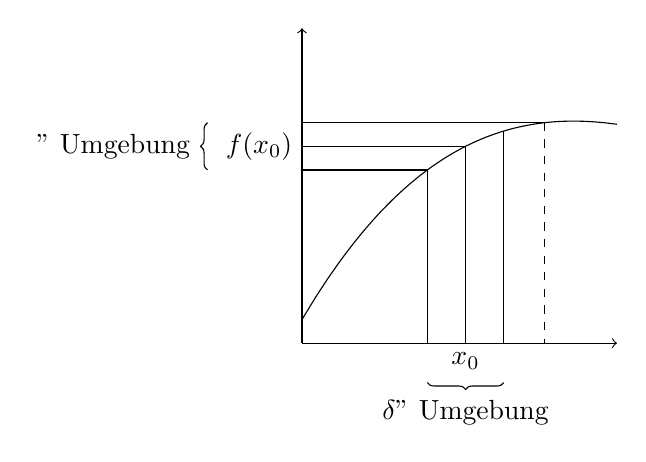
\begin{tikzpicture}
        \draw[->] (0,0) -- (4,0);
        \draw[->] (0,0) -- (0,4);

        \draw[domain=0:4, smooth] plot (\x,{0.02*(\x-5)^3-0.05*(\x-2)^2+3});
        \draw (0,2.5) node[left] {$f(x_0)$} -| (2.077,0) node[below] {$x_0$};
        \draw (0,2.8) -- (3.079,2.8);
        \draw[dashed] (3.079,2.8) -- (3.079,0);
        \draw (0,2.2) -| (1.592,0);
        \draw[decorate, decoration={brace, mirror}] (-1.2,2.8) -- (-1.2,2.2) node[midway, left, xshift=-0.1cm] {$\eps$"~Umgebung};
        \draw[decorate, decoration={brace, mirror}] (1.592,-0.5) -- (2.562,-0.5) node[midway, below, yshift=-0.1cm] {$\delta$"~Umgebung};
        \draw (2.562,0) -- (2.562,2.694);
    \end{tikzpicture}
    \caption{Darstellung des $\eps$"~$\delta$"~Kriteriums für Stetigkeit. Zu jeder $\eps$"~Umgebung finden wir eine $\delta$"~Umgebung, die innerhalb der Urbilder $f^{-1}(x_0-\eps)$ und $f^{-1}(x_0+\eps)$ liegen.}
\end{figure}

\begin{definition}[Folgenkriterium für Stetigkeit]\label{def:continuity:sequence}
    Eine Funktion $f\colon D \to \R$ heißt \emph{stetig in~$x_0 \in D$}, falls für jede Folge $(x_n)_{n\in\N}$ in~$D$ und $x_n \to x_0$ gilt $f(x_n) \to f(x_0)$. Oder anders formuliert: Für jede Folge $x_n \to x_0$ gilt
    \begin{equation*}
        \lim_{n\to\infty} f(x_n) = f\paren*{\lim_{n\to\infty} x_n}.
    \end{equation*}
\end{definition}

Die Idee der Stetigkeit ist, dass wir über eine Funktion~$f$ an einer Stelle~$x_0$ sagen können, dass sie an dem Punkt "`zusammenhängend"' ist und keine "`Sprünge"' macht. D.\,h., dass eine noch so kleine Änderung~$\eps$ um~$f(x_0)$ nur auf eine kleien Änderung~$\delta$ um~$x_0$ zurückzuführen ist bzw.\ eine $\delta$"~Änderung um~$x_0$ nur eine $\eps$"~Änderung um~$f(x_0)$ bewirkt (und keine großen wie Sprünge).

Eine ähnliche Idee beschreibt das Folgenkriterium. Laufen wir von~$-\infty$ (von links) und~$+\infty$ (von rechts) Richtung~$x_0$ und schauen uns dabei die Funktionswerte an, so können zwei Szenarien vorkommen: Treffen sich beide Grenzwerte der Funktionswerte, so gibt es keinen Sprung; treffen sie sich nicht, so gibt es einen Sprung. Viele Prozesse in der Natur sind stetig.\footnote{Letztendlich beschreibt die Stetigkeit einen Begriff der Nähe: Sind im Definitionsbereich Werte "`nah"' beinander, so sind sie auch nach Anwendung von~$f$ "`nah"' beinander. Dieser erweiterte Begriff spielt auch in der Topologie eine wichtige Rolle.}

\begin{theorem}[Äquivalenz der Stetigkeitsdefinitionen]
    \cref{def:continuity:epsdelta,def:continuity:sequence} sind äquivalent.
\end{theorem}

\begin{proof}
    Wir wollen die Funktion $f\colon D \to \R$ an~$x_0 \in D$ betrachten. Für die Äquivalenz zeigen wir die Hinrichtung und deren Kontraposition.
    
    Nehmen wir zuerst das $\eps$"~$\delta$"~Kriterium an, d.\,h.\ es gibt für jedes~$\eps > 0$ ein~$\delta > 0$, sodass für alle~$x \in \R$ mit $\abs{x-x_0} \leq \delta$ gilt: $\abs{f(x)-f(x_0)} \leq \eps$. Sei nun $(x_n)_n$ eine beliebige Folge in~$D$, die für $n \to \infty$ gegen~$x_0$ konvergiert. Aufgrund der Konvergenz finden wir für jedes gegebene~$\delta$ ein~$N \in \N$, sodass $\abs{x_n-x} \leq \delta$ für alle~$n \geq N$ ist. Insbesondere finden wir also für jedes~$\eps > 0$ ein~$N$, sodass $\abs{f(x_n)-f(x)} \leq \eps$ für alle~$n \geq N$ gilt. Damit erfüllt die Folge $(f(x_n))_n$ die Konvergenzdefinition von Folgen, also $f(x_n) \to f(x_0)$ für $n \to \infty$, was das Folgenkriterium ist.

    Für die Rückrichtung nehmen wir an, dass das Folgenkriterium nicht gelte, d.\,h.\ es gibt ein~$\eps > 0$, sodass für alle~$\delta > 0$ ein~$x$ mit $\abs{x_n-x} \leq \delta$ existiert, wofür aber $\abs{f(x)-f(x_0)} > \eps$ gilt. Wählen wir nun~$\delta = 1/n$, gibt es für jedes~$n \in \N$ ein~$x_n$ mit $\abs{x_n-x} \leq 1/n$, aber $\abs{f(x_n)-f(x)} > \eps$. Damit haben wir eine Folge~$(x_n)_n$ konstruiert, die zwar gegen~$x_0$ konvergiert, wofür aber $f(x_n) \not\to f(x_0)$ gilt. Folglich ist das Folgenkriterium nicht erfüllt.
\end{proof}

\begin{proposition}[Stetigkeit der Exponentialfunktion]
    Die Exponentialfunktion $x \mapsto \exp(x)$ ist stetig auf~$\R$.
\end{proposition}

\begin{proof}
    Mit der Restgliedabschätzung für~$\exp$ gilt für alle~$x$ mit $\abs{x-x_0} \leq 1$
    \begin{equation*}
        \abs{\exp(x)-\exp(x_0)} = \abs*{\frac{\exp(x)}{\exp(x_0)} - 1} \exp(x_0) = \abs{\exp(x-x_0)-1} \cdot \exp(x_0) \leq  2\abs{x-x_0} \cdot \exp(x_0).
    \end{equation*}
    Für jedes~$\eps > 0$ können wir ein
    \begin{equation*}
        \delta = \min\mset*{1, \frac{\eps}{2\exp(x_0)}} > 0
    \end{equation*}
    wählen, sodass für alle $\abs{x-x_0} \leq \delta$ auch die obige Ungleichung weiter durch~$\eps$ abgeschätzt werden kann.
\end{proof}

\begin{proposition}[Stetigkeit der Wurzelfunktion]
    Für alle~$k \in \N$ ist $x \mapsto x^{1/k}$ stetig auf~$\R^+$.
\end{proposition}

\begin{proof}
    Wir zeigen zunächst
    \begin{equation*}
        \abs*{x^{1/k}-x_0^{1/k}} \leq \abs{x-x_0}^{1/k}.
    \end{equation*}
    Setzen wir $y = x^{1/k}$ und $y_0 = y_0^{1/k}$, und nehmen wir o.\,B.\,d.\,A.\ $y \geq y_0$ an, gilt nach dem binomischen Lehrsatz
    \begin{equation*}
        y^k = (y_0 + (y-y_0))^k = y_0^k + \underbrace{\binom{k}{1}y_0^{k-1}(y-y_0)}_{\geq 0} + \dots + \underbrace{\binom{k}{k-1}y_0(y-y_0)^{k-1}}_{\geq 0} + y^k \geq y_0^k + (y-y_0)^k.
    \end{equation*}
    Um auch den Fall $y < y_0$ zu beachten, schreiben wir allgemeiner
    \begin{equation*}
        \abs{x-x_0} = \abs{y^k-y_0^k} \geq \abs{y-y_0}^k = \abs*{x^{1/k}-x_0^{1/k}}^k \implies \abs{x-x_0}^{1/k} \geq \abs*{x^{1/k}-x_0^{1/k}}^k.
    \end{equation*}
    Wählen wir nun $\delta = \eps^k > 0$, erhalten wir für alle~$x$ mit $\abs{x-x_0} \leq \delta$
    \begin{equation*}
        \abs*{x^{1/k}-x_0^{1/k}}^k \leq \abs{x-x_0}^{1/k} \leq \paren*{\eps^k}^{1/k} = \eps. \qedhere
    \end{equation*}
\end{proof}

\begin{proposition}
    Die konstante Funktion, die Identität und die Betragsfunktion sind stetig auf~$\R$.
\end{proposition}

\begin{proposition}[Stetigkeit unter algebraischen Operationen]
    Mit Funktionen $f$~und~$g$ sind auch die Funktionen $f+g$, $f\cdot g$ und $f/g$ (falls $g(x_0) \neq 0$) stetig in~$x_0$.
\end{proposition}

\begin{proof}
    Wir reduzieren alles auf die Grenzwertsätze von Folgen. Sei $(x_n)_n$~eine beliebige Folge mit $x_n \to x_0$. Nach Annahme gilt $f(x_n) \to f(x_0)$ und $g(x_n) \to g(x_0)$, und daher $(f+g)(x_n) \to (f+g)(x_0)$ und $(fg)(x_n) \to (fg)(x_0)$.

    Falls $g(x_0) \neq 0$, so ist auch $g(x_n) \neq 0$ für schließlich alle~$n$ und damit
    \begin{equation*}
        \paren*{\frac{f}{g}}(x_n) = \frac{f(x_n)}{g(x_n)} \to \frac{f(x_0)}{g(x_0)} = \paren*{\frac{f}{g}}(x_0). \qedhere
    \end{equation*}
\end{proof}

\begin{corollary}[Stetigkeit der Polynom"~\slash rationalen Funktion]
    Jede Polynomfunktion ist stetig auf~$\R$. Jede rationale Funktion ist stetig auf ihrem Definitionsbereich.
\end{corollary}

\begin{proposition}[Stetigkeit unter Komposition]
    Ist eine Funktion~$f\colon D \to \R$ stetig in~$x_0$ und eine Funktion~$g\colon E \to \R$ stetig in~$f(x_0)$, so ist auch $g\circ f$ stetig in~$x_0$.
\end{proposition}

\begin{proof}
    Wir benutzen das Folgenkriterium: Sei $(x_n)_n$ eine beliebige Folge in~$D$ mit $x_n \to x_0$. Aufgrund der Stetigkeit von~$f$ gilt für die Folge der~$f(x_n)$ in~$E$ auch $f(x_n) \to f(x_0)$. Wiederum wegen der Stetigkeit von~$g$ gilt für die Folge $g(f(x_n))$ auch $g(f(x_n)) \to g(f(x_0))$. Damit gilt für $x_n \to x_0$ auch $g(f(x_n)) \to g(f(x_0))$ und das Folgenkriterium in~$x_0$ ist für $g\circ f$ erfüllt.
\end{proof}

\begin{corollary}[Stetigkeit der Wurzel einer Funktion]
    Ist $f$~eine stetige Funktion, so ist auch $f^{1/k}$~stetig (in~$x_0$ bzw.\ auf~$D$).

    Insbesondere ist auch $x \mapsto x^s$ für jedes~$s \in \Q$ stetig auf~$(0,\infty)$ (bzw.\ für jedes~$s \in \Q^+$ auf~$[0,\infty)$) und $x \mapsto \abs{x}^s$ für jedes~$s \in \Q$ stetig auf $\R \setminus \mset{0}$ (bzw.\ für jedes~$s \in \Q^+$ auf~$\R$).
\end{corollary}

\lecturesep{13.~Dezember 2021}

\begin{theorem}[Zwischenwertsatz]
    Eine stetige Funktion $f\colon [a,b] \to \R$ nimmt für jeden Wert~$\gamma$ zwischen $f(a)$~und~$f(b)$ an, d.\,h.\ es gibt für jedes~$\gamma \in [f(a),f(b)]$ ein~$c \in [a,b]$ mit $f(c) = \gamma$.

    Ist insbesondere $f(a) \leq 0 \leq f(b)$, so hat $f$ eine Nullstelle.
\end{theorem}

\begin{remark}
    Der Definitionsbereich muss ein Intervall sein. Der Satz ist bspw.\ für $D = \Q \cap [a,b]$ oder für $D = [a,b] \setminus (a,b)$ falsch.
\end{remark}

\begin{proof}
    O.\,B.\,d.\,A.\ können wir annehmen, dass $f$ auf~$[a,b]$ monoton wachsend ist, also $f(a) \leq \gamma \leq f(b)$ (für monoton fallende~$f$ funktionert der Beweis analog).

    Wir definieren eine Intervallschachtelung durch Halbierung: Seien am Anfang $a_1 \coloneqq a$ und $b_1 \coloneqq b$. Danach definieren wir
    \begin{equation*}
        a_{n+1} =
        \begin{dcases}
            a_n & \text{falls } f\paren*{\frac{a_n+b_n}{2}} \geq \gamma, \\
            \frac{a_n+b_n}{2} & \text{sonst};
        \end{dcases} \qquad\qquad
        b_{n+1} =
        \begin{dcases}
            \frac{a_n+b_n}{2} & \text{falls } f\paren*{\frac{a_n+b_n}{2}} \geq \gamma, \\
            b_n & \text{sonst}.
        \end{dcases}
    \end{equation*}

    Per Induktion können wir $f(a_n) \geq \gamma \geq f(b_n)$ und $\abs{b_n-a_n} = 2^{1-n}\abs{b-a}$ für alle~$n \in \N$ zeigen (was relativ einfach ist). Aus dem Intervallschachtelungsprinzip folgt nun, dass es ein~$c$ gibt mit
    \begin{equation*}
        c = \lim_{n\to\infty} a_n = \lim_{n\to\infty} b_n.
    \end{equation*}
    Aus der Stetigkeit via Folgenkriterium und dem Sandwichlemma folgt
    \begin{equation*}
        f(a_n) \leq \gamma \leq f(b_n) \implies f(c) = \lim_{n\to\infty} f(a_n) \leq \gamma \leq \lim_{n\to\infty} = f(c) \implies f(c) = \gamma. \qedhere
    \end{equation*}
\end{proof}

Der Zwischenwertsatz ist sehr mächtig, da wir mit ihm Aussagen über die Bildmenge einer stetigen Funktion machen können und daraus auch einige Eigenschaften ermitteln können.

\begin{corollary}
    Jedes Polynom ungeraden Grades, also
    \begin{equation*}
        f\colon \R \to \R \quad\text{mit}\quad f(x) = a_{2n+1}x^{2n+1} + a_{2n}x^{2n} + \dots + a_0 \quad\text{mit } a_{2n+1} \neq 0,
    \end{equation*}
    hat mindestens eine \emph{reelle} Nullstelle
\end{corollary}

\begin{proof}
    O.\,B.\,d.\,A.\ sei $a_{2n+1} > 0$. Dann konvergieren die Funktionswerte uneigentlich: $\lim_{n\to\infty} f(x) = \infty$ und $\lim_{n\to-\infty} f(x) = -\infty$. Folglich gibt es reelle Zahlen $a,b \in \R$ mit $a < b$ und $f(a) < 0 < f(b)$. Damit existiert eine Nullstelle in~$[a,b]$.
\end{proof}

\begin{corollary}\label{cor:continuity:interval}
    Sei $I \in \R$ ein beliebiges Intervall (offen, abgeschlossen, halboffen, beschränkt, unbeschränkt). Ist eine Funktion $f\colon I \to \R$ stetig auf~$I$, so ist auch $f(I)$~ein Intervall.
\end{corollary}

\begin{proof}
    Für~$I = \varnothing$ ist offensichtlich $f(I) = \varnothing \subset \R$ auch ein "`Intervall"'. Deshalb nehmen wir o.\,B.\,d.\,A.\ $I \neq \varnothing$ an. Für~$I = [x,x]$ ist auch offensichtlich $f(I) = [f(x),f(x)]$ ein Intervall. Deshalb nehmen wir auch $\diam(I) > 0$ an.

    Seien $A = \inf f(I) \in [-\infty,\infty)$ und $B = \sup f(I) \in (-\infty,\infty]$ (in~$\exR$). Für jedes~$\gamma \in (A,B)$ gibt es $a,b \in I$ mit $f(a) < \gamma < f(b)$. Weil $f$ insbesondere auf~$(a,b)$ stetig ist, gibt es nach Zwischenwertsatz ein~$c \in I$ mit~$f(c) = \gamma$. Daraus folgt $\gamma \in f(I)$ für alle~$\gamma \in (A,B)$, oder $(A,B) \subset f(I) \subset ([A,B] \cap \R)$ (geschnitten mit~$\R$, da wir nicht erlauben wollen, dass $\pm\infty \in f(I)$). Somit haben wir~$f(I)$ geschachtelt, und $f(I)$ kann nur eines von $(A,B)$, $[A,B]$, $(A,B]$ oder~$[A,B)$ (geschnitten mit~$\R$) sein.
\end{proof}

Der Grund, wieso wir nochmals $a$~und~$b$ einführen mussten ist, dass $A$~und~$B$ nicht notwendigerweise Funktionswerte sein müssen.

\begin{definition}[kompaktes Intervall]
    Ein Intervall~$I \subset \R$ heißt \emph{kompakt}, falls es abgeschlossen und beschränkt ist.
\end{definition}

\begin{theorem}[Extremwertsatz]
    Das Bild eines kompakten Intervalls unter einer stetigen Abbildung ist ein kompaktes Intervall. Insbesondere nimmt jede stetge Funktion auf einem kompakten Intervall ihre Extrema an, d.\,h.\ für ein stetiges $f\colon I \to \R$ mit~$I \subset \R$ kompakt gibt es $p,q \in I$ mit
    \begin{equation*}
        f(p) = \sup f(I) \qquad\text{und}\qquad f(q) = \inf f(I).
    \end{equation*}
    Oder mit anderen Worten: Es existieren $p,q \in I$, sodass $f(y) \leq f(x) \leq f(p)$ für alle~$x \in I$ gilt und damit $f(I) = [f(q),f(p)]$.
\end{theorem}

\begin{remark}
    Der Satz stimmt für offene/halboffene Intervalle nicht. Bspw.\ ist $f\colon x \mapsto 1/x$ auf~$I = (0, 1]$ definiert, wobei $I$~beschränkt ist. Aber $f(I) = [1,\infty)$ ist ein \emph{unbeschränktes} Intervall, d.\,h.\ es gibt \underline{kein}~$p \in I$ mit $f(p) = \infty \notin \R$.
\end{remark}

\begin{proof}[Beweis des Extremwertsatzes]
    Sei $I$~ein kompaktes Intervall und $f\colon I \to \R$ eine stetige Funktion. Seien $A = \inf f(I)$ und $B = \sup f(I)$ (wobei $A,B \in \exR$). Dann existieren Folgen $(a_n)_n$~und~$(b_n)_n$ in~$I$ mit $f(a_n) \to A$ und $f(b_n) \to B$.\footnote{Leider hat auch hier der Dozent eine Aussage verwendet, die wir noch nicht bewiesen haben: Ist~$M \subset \R$, so gibt es eine Folge~$(a_n)_{n\in\N}$ mit~$a_n \in M$ für alle~$n$ und $a_n \to \sup M$. \emph{Beweis}: Für jedes~$n \in \N$ muss es ein~$a_n \in M$ mit $\sup M - 1/n \leq a_n$ geben; andernfalls wäre $\sup M - 1/n$ eine kleinere obere Schranke als~$\sup M$. Nun gilt auch $a_n \leq \sup M$, also $a_n \to \sup M$ nach dem Sandwichlemma.}
    
    Dabei sind die Folgen $(a_n)_n$~und~$(b_n)_n$ beschränkt, da $I$~beschränkt ist. Folglich können wir den Satz von Bolzano-Weierstraß anwenden, sodass $(a_n)_n$~und~$(b_n)_n$ einen Häufungspunkt $q$~bzw.~$p$ besitzen, d.\,h.\ es gibt Teilfolgen $(a_{n_k})_k$~und~$(b_{n_k})_k$ mit $a_{n_k} \to q$ bzw.\ $b_{n_k} \to p$.

    Wegen der Abgeschlossenheit von~$I$ ist $p,q \in I$ und $f$~ist in $p$~und~$q$ definiert. Weil in einer konvergenten Folge jede Teilfolge gegen denselben Grenzwert konvergiert, folgt aus der Stetigkeit von~$f$
    \begin{gather*}
        A = \lim_{n\to\infty} f(a_n) = \lim_{n\to\infty} f(a_{n_k}) = f\paren*{\lim_{n\to\infty} a_{n_k}} = f(q)
        \shortintertext{und analog}
        B = \lim_{n\to\infty} f(b_{n_k}) = f(p).
    \end{gather*}
    Wegen dem Zwischenwertsatz gilt $[f(p),f(q)] \subset f(I) \subset [A,B]$ und damit $f(I) = [f(q),f(p)]$.
\end{proof}

\begin{definition}[gleichmäßige Stetigkeit]
    Eine Funktion $f\colon D \to \R$ heißt \emph{gleichmäßig stetig}, falls für jedes~$\eps > 0$ ein~$\delta > 0$ existiert, sodass
    \begin{equation*}
        \abs{f(x)-f(x_0)} \leq \eps \qquad\text{für alle } x,x_0 \in D \text{ mit } \abs{x-x_0} \leq \delta
    \end{equation*}
    gilt. Oder in Zeichen:
    \begin{equation*}
        \forall \eps > 0\colon \exists \delta > 0\colon \forall x,x_0 \in D\colon\quad \abs{x-x_0} \leq \delta \implies \abs{f(x)-f(x_0)} \leq \eps.
    \end{equation*}
\end{definition}

\begin{remark}\label{rem:uniformcontinuity}
    Wenn wir uns die Definition der Stetigkeit
    \begin{equation*}
        \forall x_0 \in D\colon \forall \eps > 0\colon \exists \delta > 0\colon \forall x \in D\colon\quad \abs{x-x_0} \leq \delta \implies \abs{f(x)-f(x_0)} \leq \eps
    \end{equation*}
    anschauen, so ist das $\forall x_0 \in D$ nach Innen gerutscht. Das bedeutet, dass $\delta$ bei der gleichmäßigen Stetigkeit nur noch von~$\eps$ abhängen darf, wohingegen $\delta$ bei der (punktweisen) Stetigkeit von~$\eps$ und~$x_0$ abhängen durfte.

    Damit ist die gleichmäßge Stetigkeit eine stärkere Bedingung, und sie impliziert auch die einfache Stetigkeit.\footnote{Wir können den Unterschied auch im Sinne von Approximation verstehen: Bei der Stetigkeit können wir für jede Stelle~$x_0$ und jeden Maximalfehler~$\eps$ in den Funktionswerten eine $\delta$"~Umgebung finden, sodass der Fehler in dieser Umgebung kleiner~$\eps$ ist, d.\,h.\ die~$f(x)$ mit~$x \in [x_0-\delta,x_0+\delta]$ approximieren $f(x_0)$ gut. Dabei kann aber die $\delta$"~Umgebung von~$x_0$ abhängen.
    
    Bei der gleichmäßigen Stetigkeit haben wir hingegen eine gleichmäßige Approximation: Für jeden Maximalfehler~$\eps$ gibt es ein~$\delta$, sodass wir uns sicher sein können, dass die $\delta$"~Umgebung um \emph{jede Stelle~$x_0$} ausreichend gute Approximation ist.
    
    Eine weitere Eigenschaft: Jede Cauchy-Folge bleibt unter einer gleichmäßig stetigen Funktion wieder eine Cauchy-Folge, was wir bei punktweiser Stetigkeit nicht behaupten können.}
\end{remark}

\begin{theorem}
    Sei $I$~ein kompaktes Intervall. Dann ist die Funktion $f\colon I \to \R$ genau dann stetig, wenn sie gleichmäßig stetig ist.\footnote{Der Satz ist auch als \emph{Satz von \textsc{Heine}} bekannt.}
\end{theorem}

\begin{proof}
    Die Rückrichtung ist trivial (s.~\cref{rem:uniformcontinuity}).

    Die Hinrichtung zeigen wir indirekt: Angenommen $f$~ist nicht gleichmäßig stetig, d.\,h.\ es gibt ein~$\eps > 0$, sodass für jedes~$\delta = 1/n > 0$ Stellen $x_n,y_n \in I$ mit $\abs{x_n-y_n} \leq \delta = 1/n$ und $\abs{f(x_n)-f(y_n)} > \eps$ gibt.

    $(x_n)_n$~und~$(y_n)_n$ sind Folgen in~$I$ und damit beschränkt. Mit dem Satz von Bolzano-Weierstraß gibt es eine Teilfolge~$(x_{n_k})_k$ mit $x_{n_k} \to p \in I$ (ein Häufungspunkt). Aus der Bedingung $\abs{x_n-y_n} \leq 1/n$ folgt $y_{n_k}-x_{n_k} \to 0$, also $y_{n_k} \to p$. Aufgrund Stetigkeit von~$f$ erhalten wir
    \begin{equation*}
        f(y_{n_k}) - f(x_{n_k}) \to f(p) - f(p) = 0,
    \end{equation*}
    ein Widerspruch zur Annahme $\abs{f(y_{n_k})-f(x_{n_k})} > \eps$ für alle~$k \in \N$.
\end{proof}

\begin{example}\leavevmode
    \begin{enumerate}
        \item Die Funktion $x \mapsto \sin(1/x)$ auf $(0, 1] \subset \R$ ist \emph{nicht} gleichmäßig stetig.
        \begin{center}
            \begin{tikzpicture}
                \draw[->] (0,0) -- (2.5,0);
                \draw[->] (0,-1.5) -- (0,1.5);
                \pic at (0,1) {ytick=1};
                \pic at (0,0) {ytick=0};
                \pic at (0,-1) {ytick=$-1$};
                \draw[domain=0.01:1, smooth, samples=2000] plot (2*\x,{sin((1/\x)r)});
            \end{tikzpicture}
        \end{center}
        \item Die Funktion $x \mapsto 1/x$ auf~$I = (0, 1]$ ist zwar stetig, aber nicht gleichmäßig stetig, denn für~$\eps = 1$ gibt es für jedes~$\delta > 0$ Stellen $x = \min\mset{\frac{1}{2},\delta} \in I$ und~$x' = 2x \in I$ mit $\abs{x-x'} = x \leq \delta$, aber $\abs{f(x)-f(x')} = 1/(2x) \geq 1 = \eps$.
        \item Die \emph{Verteilungsfunktion auf der \textsc{Cantor}-Menge} bzw.\ \emph{\textsc{Cantor}-Verteilung} (auch engl.\ \emph{devil's staircase}) auf~$[0, 1]$ ist gleichmäßig stetig.
        
        Die Funktionen wird über die rekursiv definierten Cantor-Mengen konstruiert. Das Intervall~$[0, 1]$ wird gedrittelt, wobei für das mittlere Drittel~$(\frac{1}{3},\frac{2}{3})$ die Funktion den Wert~$\frac{1}{2}$ annimmt. Dann bleiben noch das linke Drittel~$L = [0,\frac{1}{3}]$ und das rechte Drittel~$R = [\frac{2}{3},1]$ übrig. Auf diesen beiden Machen wir dieselbe Konstruktion, wobei das mittlere Drittel von~$L$ den Wert~$\frac{1}{4}$, das mittlere Drittel von~$R$ den Wert~$\frac{3}{4}$ annimmt. Das können wir so fortführen.
        \begin{center}
            \begin{tikzpicture}[scale=3]
                \draw[->] (0,0) -- (1.2,0);
                \draw[->] (0,0) -- (0,1.2);
                \pic at (0,0.25) {ytick=$\frac{1}{4}$};
                \pic at (0,0.5) {ytick=$\frac{1}{2}$};
                \pic at (0,0.75) {ytick=$\frac{3}{4}$};
                \pic at (0,1) {ytick=1};
                \pic at (1/3,0) {xtick=$\frac{1}{3}$};
                \pic at (2/3,0) {xtick=$\frac{2}{3}$};
                \pic at (1,0) {xtick=1};
                \tikzmath{
                    function cantor(\i, \xstart, \xend, \ymin, \ymax) {
                        \xleft = \xstart + (\xend-\xstart)/3;
                        \xright = \xend - (\xend-\xstart)/3;
                        \ymid = \ymin + (\ymax-\ymin)/2;
                        {\draw (\xleft,\ymid) -- (\xright,\ymid);};
                        if (\i > 0) then {
                            cantor(\i-1,\xstart,\xleft,\ymin,\ymid);
                            cantor(\i-1,\xright,\xend,\ymid,\ymax);
                        };
                    };
                    cantor(7,0,1,0,1);
                }
            \end{tikzpicture}
        \end{center}
        Nach dem $k$"~ten Schritt ist kein "`Sprung"' größer als~$2^{-k}$.
    \end{enumerate}
\end{example}

\begin{theorem}
    Sei~$D \subset \R$ ein Intervall und $f\colon D \to \R$ stetig und strikt monoton. Dann bildet~$f$ das Intervall~$D$ bijektiv auf das Intervall~$D' = f(D)$ ab und die Umkehrfunktion $f^{-1}\colon D' \to \R$ ist stetig und strikt monoton.
\end{theorem}

\begin{proof}
    Wegen \cref{cor:continuity:interval} ist $D'$~ein Intervall. Weil $f$~strikt monoton, ist es auch injektiv. Zusammen ist also $f\colon D \to D'$ bijektiv. Folglich existiert $f^{-1}\colon D' \to D$ und ist strikt monton, denn für z.\,B.\ monoton wachsende Funktion gilt $x < y \iff f(x) < f(y) \iff f^{-1}(f(x)) < f^{-1}(f(y))$ und analog für monoton fallende.

    Nun müssen wir nur noch die Stetigkeit zeigen, die wir indirekt mittels dem Folgenkriterium zeigen wollen. Angenommen es gäbe eine Stelle~$y \in D'$, in der $f^{-1}$~nicht stetig wäre, d.\,h.\ es gibt eine Folge~$(y_n)_n$ in~$D'$ mit $y_n \to y$, wofür $x_n \coloneqq f^{-1}(y_n) \not\to f^{-1}(y) \eqqcolon x$ gilt. Weil $(y_n)_n$~konvergiert, ist die Folge beschränkt (\cref{thm:bound}). Damit gibt es ein kompaktes Intervall~$f(D_0)$ mit~$D_0 \subset I$, das alle~$y_n$ enthält. Aufgrund der Monotonie muss auch $D_0$~selbst kompakt sein, d.\,h.\ $(x_n)_n$~ist beschränkt. Nach Bolzano-Weierstraß gibt es eine konvergente Teilfolge $x_{n_k} \to \bar{x} \in D_0$ mit~$\bar{x} \neq x$, denn $(x_n)_n$~konvergiert nicht, sodass es mindestens zwei verschiedene Häufungspunkte geben muss. Daraus folgt aufgrund der Stetigkeit von~$f$ nun
    \begin{equation*}
        f(\bar{x}) = \lim_{n\to\infty} f(x_{n_k}) = \lim_{n\to\infty} y_{n_k} = y = f(x),
    \end{equation*}
    und aufgrund Bijektivität $\bar{x} = x$, ein Widerspruch.
\end{proof}

\begin{example}
    Für~$k \in \N$ ist die Potenzfunktion $f\colon \R^+ \to \R^+$, $x \mapsto x^k$ strikt monoton wachsend und stetig. Sie bildet $\R^+$ also bijektiv auf~$\R^+$ ab. Die Umkehrfunktion ist die $k$"~te Wurzel $x \mapsto x^{1/k} = \sqrt[k]{x}$.

    Für ungerade~$k$ ist $x \mapsto x^k$ auf ganz~$\R$ strikt monoton. Somit können wir $x \mapsto x^{1/k}$ auf ganz~$\R$ definieren.
    \begin{center}
        \begin{tikzpicture}[baseline=(current bounding box.base)]
            \draw[->] (-0.5,0) -- (2,0) node[below] {$x$};
            \draw[->] (0,-0.5) -- (0,2.5) node[left] {$y$};
            \draw[domain=0:1.5, smooth] plot (\x,\x^2) node[right] {$x^2$};
        \end{tikzpicture}
        \hspace*{0.4cm}
        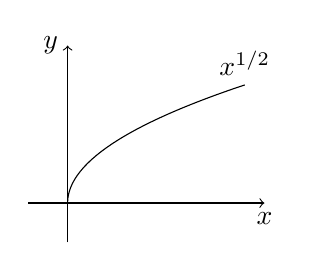
\begin{tikzpicture}[baseline=(current bounding box.base)]
            \draw[->] (-0.5,0) -- (2.5,0) node[below] {$x$};
            \draw[->] (0,-0.5) -- (0,2) node[left] {$y$};
            \draw[domain=0:1.5, smooth] plot (\x^2,\x) node[above] {$x^{1/2}$};
        \end{tikzpicture}
        \hspace*{0.4cm}
        \begin{tikzpicture}[baseline=(current bounding box.base)]
            \draw[->] (-1.7,0) -- (1.7,0) node[below] {$x$};
            \draw[->] (0,-2.5) -- (0,2.5) node[left] {$y$};
            \draw[domain=-1.3:1.3, smooth] plot (\x,\x^3) node[right] {$x^3$};
        \end{tikzpicture}
        \hspace*{0.4cm}
        \begin{tikzpicture}[baseline=(current bounding box.base)]
            \draw[->] (-2.5,0) -- (2.5,0) node[below] {$x$};
            \draw[->] (0,-1.7) -- (0,1.7) node[left] {$y$};
            \draw[domain=-1.3:1.3, smooth] plot (\x^3,\x) node[above] {$x^{1/3}$};
        \end{tikzpicture}
    \end{center}
\end{example}

\lecturesep{15.~Dezember 2021}

\newpage\appendix

\section{Trickkiste}

Wie löse ich eine Aufgabe? Das sollte für Mathematikstudenten eine sehr wichtige Frage sein. Es gibt eigentlich zwei Antworten:
\begin{itemize}
    \item Es gibt generelle Problemlösestrategien, die auf jeder Aufgabe anwendbar sind. Im Englischen werden Leute, die gut darin sind, als \emph{problem solver} bezeichnet.

          Ich fasse mal ein paar dieser Strategien in Fragen zusammen:
          \begin{itemize}
              \item Wo habe ich das schon einmal gesehen? Woran erinnert mich die Aufgabe?
              \item Kann ich eine Analogie machen oder eine Veranschaulichung zeichnen?
              \item Was ist gegeben? Was kann ich aus dem Gegebenen schlussfolgern?
              \item Was ist gesucht? Welche Aussagen muss ich davor zeigen, um zum gesuchten Ergebnis zu kommen? (Diese und die vorherige Frage komplementieren sich, sodass man durch wiederholtes Vorwärts"~ und Rückwärtsarbeiten womöglich beide Enden in der Mitte zu einer Lösung zusammenführen.)
              \item Kann ich mir ein konkretes Beispiel/einen konkreten Fall anschauen und die Aufgabe dafür lösen (\emph{toy problems})? Was beobachte ich? Kann ich den Beweis verallgemeinern?
              \item Kann ich eine Lösung/ein Beispiel raten? Welche Heuristiken könnte ich verwenden, um die Lösungssuche zu vereinfachen (das ist die Definition einer Heuristik)? Wie müsste eine Lösung wahrscheinlich aussehen?
              \item Und noch weitere Strategien. An dieser Stelle ist \textsc{George Pólyas} \emph{Schule des Denkens: Vom lösen mathematischer Probleme ("`How to solve it"').} zu empfehlen.
          \end{itemize}

    \item Es gibt gewisse mathematische Tricks (sie wirken wie Zauberei, sind aber trotzdem mathematisch korrekt), die in spezifischen Aufgaben oder Aufgabentypen Anwendung finden. Oft sind sie die Idee, die man haben muss, um auf die Lösung zu kommen, und nur manchmal gibt es alternative \emph{brute force}"=Lösungswege.

          Was man sich beim anschauen der Musterlösung oder Lösung anderer fragen sollte ist: Was war der Trick? Wie hätte ich darauf kommen können? Auf welche Arten von Aufgaben kann ich den Trick anwenden? Worauf müsste ich achten, um mich an diesen Trick zu erinnern?

          Diese Sammlung von Tricks habe ich immer meine \emph{mathematische Trickkiste} genannt~-- andere nennen sie vielleicht \emph{Werkzeugkasten} oder \emph{dreckige Tricks}, aber ich bleibe bei der Trickkiste. Diese Tricks sind oftmals nicht spezifisch für einen mathematischen Fachbereich, sondern können auch in anderen Bereichen Anwendung finden.
\end{itemize}

Die folgende Zusammenstellung ist (wie es sich für einen aktiv genutzten Werkzeugkasten gehört) nicht sehr strukturiert. Und leider ist es so, dass man erst ein Werkzeug richtig versteht, wenn man es im Kontext nutzt und sieht, also \emph{üben, üben, üben!}

\subsection{Logik und Mengenlehre}

\subsection{Sonstiges}

\begin{itemize}
    \item Es ist extrem wichtig, sicher in Termumformungen zu sein. Dazu gehören Ausmultiplizieren, Gleichungen und Ungleichungen äquivalent umformen, die binomischen Formeln und der binomische Lehrsatz, Potenz"~ und Wurzelgesetze, Rechnen mit Brüchen, etc.\,pp.
    \item Ausklammern und Faktorisieren ist auch sehr nützlich, aber ungemein schwerer.
          \begin{itemize}
              \item Man kennt vielleicht einfach die Faktorisierung. Dazu sollten gehören:
                    \begin{itemize}
                        \item die binomischen Formeln (auch $x^2 \pm 2x + 1 = (x \pm 1)^2$ und $x^2 - 1 = (x+1)(x-1)$),
                        \item der binomische Lehrsatz, insbesondere auch $(x + y)^3 = x^3 + 3x^2y + 3xy^2 + y^3$,
                        \item $x^3 - y^3 = (x^2 + xy + y^2)$,
                        \item $x^n - y^n = (x-y) (x^{n-1} + x^{n-2}y + x^{n-3}y^2 + \dots + y^{n-1})$,
                        \item $x^n + y^n = (x+y) (x^{n-1} - x^{n-2}y + x^{n-3}y^2 - x^{n-4}y^3 + \dots + y^{n-1})$ für ungerade~$n$.
                    \end{itemize}
              \item Man kann und sollte manchmal auch raten.
                    \begin{itemize}
                        \item Z.\,B.\ indem man sich den Grad des zu faktorisierenden Terms anschaut, und dann überlegt, welchen Grad die Faktoren haben müssen. Bspw.\ $x^3 - y^3 = (x - y) (x^2 + xy + y^2)$; links steht Grad~3, rechts zwei Faktoren mit Grad~1 und Grad~2.
                        \item Ein nützlicher Trick ist das Raten von Nullstellen~$x_0$ von Polynomen in~$x$, sodass dieser als Faktor $x - x_0$ ausgeklammert werden kann. Bspw.\ hat $p = x^3 - 3x - 2$ die Nullstelle $x_0 = -1$, sodass $p$~einen Faktor $x-x_0 = x+1$ hat, d.\,h.\ $p = (x+1) (x^2 - x + -2)$. Der zweite Faktor hat wiederum einen Faktor $x_0 = 2$ und daher $p = (x+1) (x-2) (x+1)$. Wir hätten also auch noch einmal $x_0 = 1$ als Nullstelle raten können.
                        \item Natürlich sollte man beim Raten auch sein Gehirn ein wenig einschalten um zu schauen, welche Terme in den Faktoren da sein müssen, um den ursprünglichen Term zu erhalten.
                    \end{itemize}
              \item Substitution sollte man auch sehen können, wie z.\,B.\ $(x^2 + y^2)^2 = x^4 + 2x^2y^2 + y^4$, was $(a + b)^2$ für~$a = x^2$ und~$b = y^2$ ist.
          \end{itemize}
\end{itemize}

\section{Halmos' \emph{Naive Mengenlehre} über die russellsche Antinomie}\label{apx:russell}

\textsc{Halmos'} \emph{Naive Mengenlehre}\footnote{\textsc{Halmos, Paul R.}, \textsc{Ostermann, Fritz}~\& \textsc{Armbrust, Manfred} (Übers.): \textit{Naive Mengenlehre.} Göttingen~1968: Vandenhoeck~\& Ruprecht, 2.~Auflg. Kap.~2, S.~19f.} behandelt die \textsc{russellsche} Antinomie. Hier ein Auszug:

\begin{quotation}
    \textbf{Aussonderungsaxiom}: \emph{Zu jeder Menge~$A$ und jeder Bedingung~$S(x)$ gibt es eine Menge~$B$, deren Elemente genau jene~$x$ aus~$A$ sind, für die~$S(x)$ gilt.}~[\dots]

    Man erhält eine amüsante und zugleich recht lehrreiche Anwendung des Aussonderungsaxioms, wenn man für~$S(x)$ die Aussage
    \begin{equation*}
        \text{nicht } (x \in x)
    \end{equation*}
    [$x \notin x$] setzt.~[\dots] Unabhängig von der vorgegebenen Menge~$A$ folgt: wenn $B = \mset{x \in A : x \notin x}$, so gilt für alle~$y$
    \begin{equation}
        y \in B \text{ \emph{dann und nur dann, wenn} } (y \in A \text{ \emph{und} } y \notin y). \tag*{$(*)$}\label{eqn:halmos}
    \end{equation}
    Kann~$B \in A$ gelten? Die Antwort heißt nein! Selbstverständlich gilt entweder~$B \in B$ (ungewöhnlich, aber nicht offenkundig unmöglich), oder~$B \notin B$; im Falle~$B \in A$ würde aber aus~$B \in B$ auf Grund von~\ref{eqn:halmos} $B \notin B$ folgen, also ein Widerpsruch, anderserseits aus~$B \notin B$ ebenfalls nach~\ref{eqn:halmos} $B \in B$, also abermals ein Widerspruch. Demnach kann auf keinen Fall~$B \in A$ gelten, also haben wir~$B \notin A$. Das Interessante an dieser Folgerung ist die Feststellung, daß es etwas gibt (nämlich~$B$), das nicht zu~$A$ gehört; die Menge~$A$ war bei dieser Betrachtung völlig beliebig. Damit haben wir mit anderen Worten bewiesen:
    \begin{center}
        \textit{keine Menge enthält alles,}
    \end{center}
    oder eindrucksvoller:
    \begin{center}
        \textit{es gibt keine Allmenge.}
    \end{center}
    Noch anders gewendet: eine Gesamtheit, die alle Objekte (Mengen) unserer Theorie enthalten würde, könnte nicht selbst Objekt unserer Theorie sein.

    In älteren (präaxiomatischen) Zugängen zur Mengenlehre hatte man die Existenz einer Allmenge als selbstverständlich angenommen und damit auch naiv geglaubt, daß jede Aussage~$S(x)$ im absoluten Sinne, nämlich in der vermeintlichen Allmenge, eine "`Erfüllungs"'"~Menge bestimme. In obiger Argumentation fällt dann aber bei der Definition von~$B$, also auch in~\ref{eqn:halmos}, der Zusatz~$x \in A$ (bzw.~$y \in A$) fort, und es offenbart sich an der Frage, ob~$B \in B$ oder~$B \notin B$, ein eklatanter Widerspruch in der Theorie, bekannt als \emph{Russelsche Paradoxie}. Die Nutzanwendung liegt darin, daß es --~insbesondere in der Mathematik~-- unmöglich ist, aus dem Nichts etws zu schaffen. Zur Beschreibung einer Menge genügt es also nicht, ein paar magische Worte auszusprechen (selbst wenn sie eine formal richtig gebildete Aussage wie "`$x \notin x$"' darstellen), sondern man muß schon eine Menge zur Verfügung haben (in unserer Argumentation hieß sie~$A$) auf deren Elemente sich die magischen Worte anwenden lassen.
\end{quotation}

\end{document}
